\chapter{Dedicated Control Regions}
\label{ch:control_regions}
\epigraph{\itshape``Noise proves nothing. Often a hen who has merely laid an egg cackles as if she laid an asteroid."}{--- \textup{Mark Twain}}

\section{Introduction}
\hspace{10pt} The approach taken for the estimation of the main sources of backgrounds, originating from V+jets SM processes, is to use a set of dedicated control regions (CR) representing each of these processes. The irreducible contribution of these Z$(\nu\nu)$+jets and W($l\nu$)+jets (where the charged lepton is unidentified by the detector) SM background are estimated using a set of well identified lepton regions that are associated with the same dijet properties as the ones used for the definition of both SR categories.

\hspace{10pt} Regions are selected to be orthogonal to each other, bearing similarities to the SR in order to ensure a smooth transition between the information gained from the CR and the final estimation in the SR. The main help with this approach is the usage of $E_{T, miss}$ where the leptons have been removed from the computation (as previously defined in Section~\ref{subsec:mtr_triggers}), which further helps with the preservation of the VBF-like selection. Following sections will further explain the definition of each of these regions.

\hspace{10pt} In addition to the main V+jets backgrounds, there is one more SM source of background noise that requires special attention. The QCD multijet processes present a problem due to the lack of statistics in their corresponding simulation samples, requiring an estimation from regions enriched with contributions from these processes. The formation of the of these dedicated QCD enriched regions and the methodology behind their usage in the final extrapolation to the SR are also going to be the focus of few of the following pages.

\section{Lepton Regions}
\hspace{10pt} Focusing on regions dedicated to the estimation of V+jets influence on the SR, upcoming pages are going to introduce the four main lepton CRs, which can be grouped into two categories based on their targeted processes: the double and single lepton CRs. The idea behind the double lepton regions is to provide a good handle when tackling the Z$(\nu\nu)$+jets processes, while the single lepton regions take over the responsibilities associated with the W($l\nu$)+jets processes. Their respective definitions, focusing on further separation using lepton flavour, are going to be summarised in the following sections.

\subsection{Double Muon CR}
\hspace{10pt} As illustrated in the introduction, the double muon CR aims to help with the Z$(\nu\nu)$+jets processes. This region is formed by replacing the muon veto selection requirement from VTR and MTR selections (Tables~\ref{tab:selection_mtr} and~\ref{tab:selection_vtr}) with a requirement that there are exactly two muon objects in the event. At least one of these two objects must pass the tight requirements defined in Section~\ref{sec:objects}. Additional selection requirements are imposed on muon $p_T$ with thresholds being set at $p_T>$20/10~GeV for the leading/subleading muon respectively (being connected to the tight muon requirements). The final item is related to the formation of a dilepton mass region around the value of the Z boson mass, imposing a 60~$<m_{ll}<$~120~GeV requirement.

\hspace{10pt} Figures~\ref{fig:2017_Zmumu_1} and~\ref{fig:2018_Zmumu_1} show the distributions of invariant masses of dilepton and dijet objects for both the MTR and VTR selection for both 2017 and 2018 eras. Overall good data to simulation agreement is reported for both variables in all categories, with the agreement being within the values controlled by the final fit. The much lower statistics of the VTR category originates from a set of higher $p_T$ thresholds included in VTR selection requirements.

\hspace{10pt} Figures~\ref{fig:2017_Zmumu_2} and~\ref{fig:2018_Zmumu_2} are showing the $min\Delta\phi(j, E_{T,miss}^{no,\mu})$ and $E_{T,miss}^{no,\mu}$ variables for both categories for the 2017 and 2018 eras of data taking, respectively. The inclusion of tight muon requirements as well as the constrain being put on the dimuon mass has helped with removing contributions from additional effects.

\begin{figure}[htbp]
  \centering
    \subfigure[$m_{ll}$ - MTR]{
    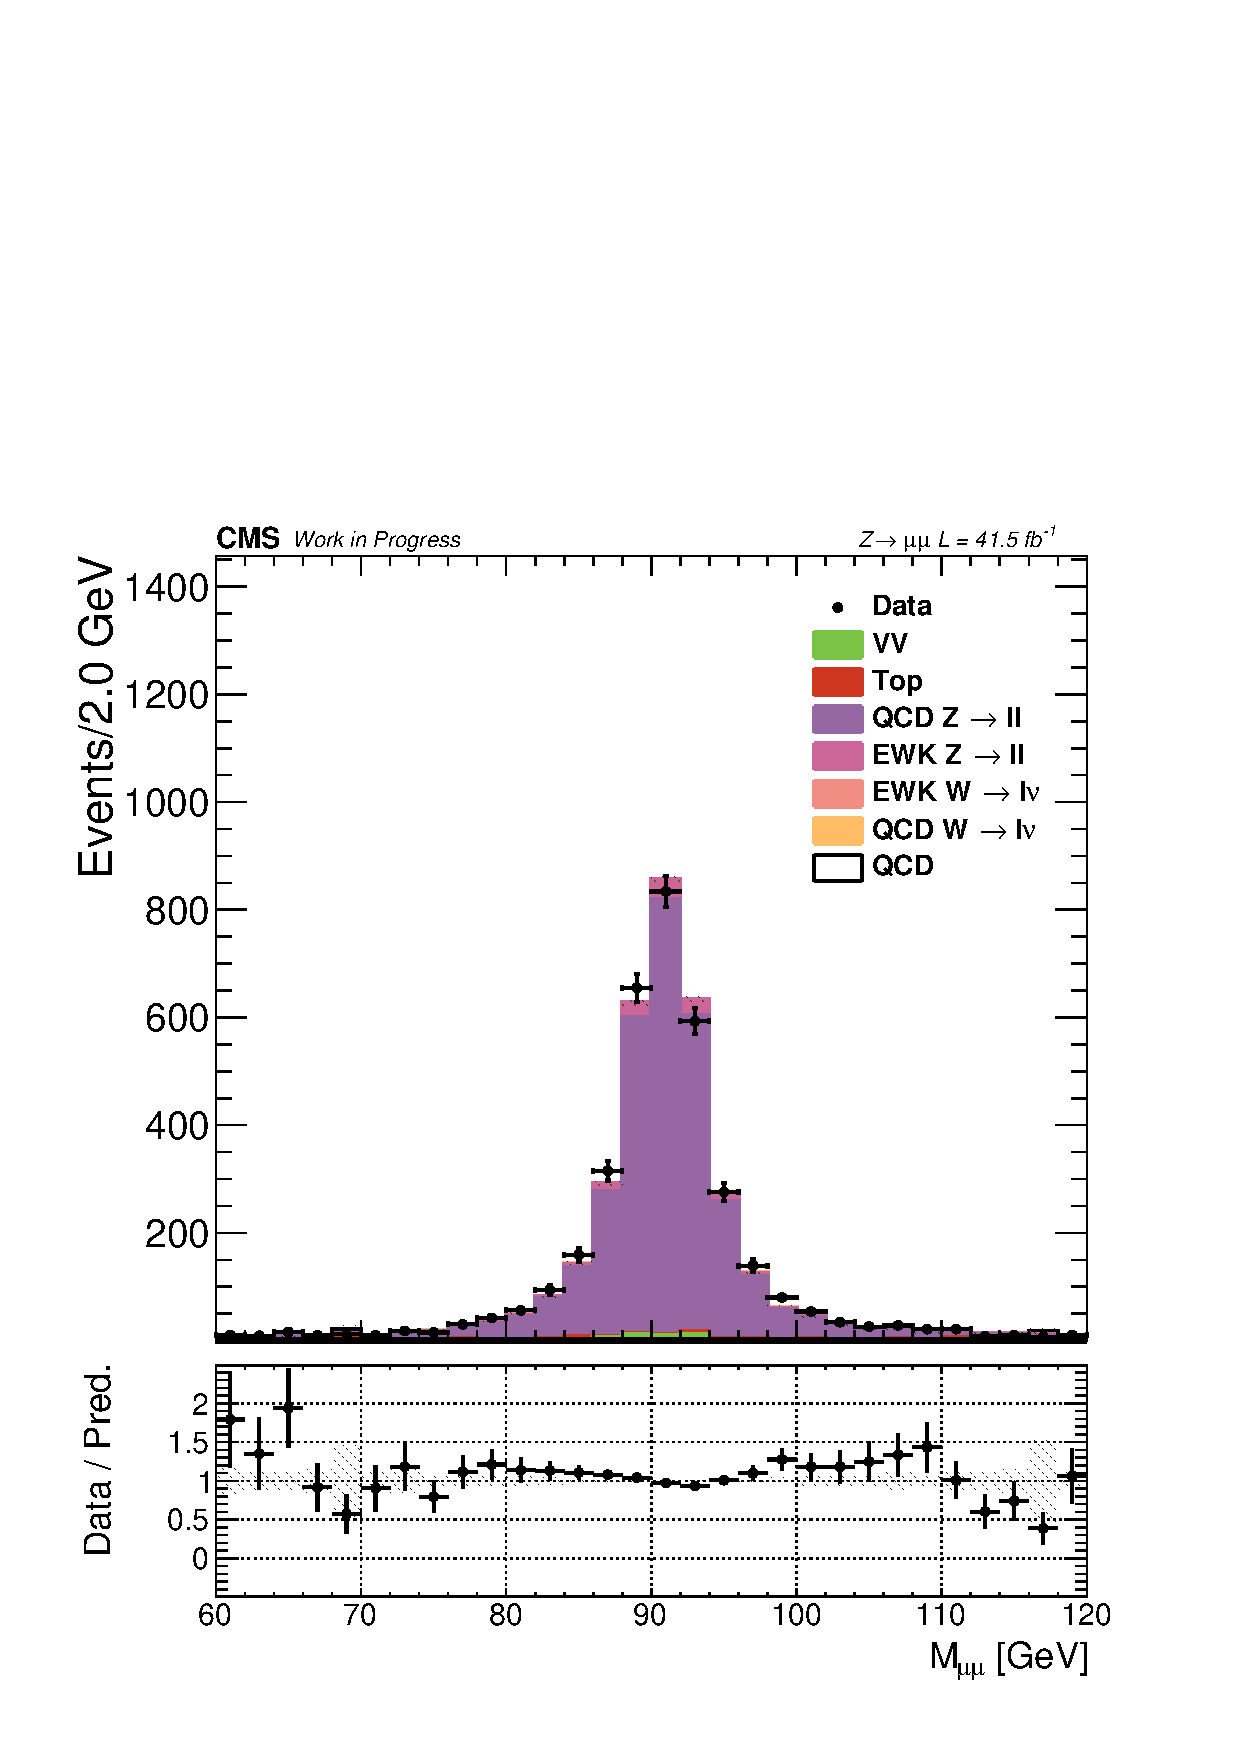
\includegraphics[width=0.49\textwidth]{Control_Regions/2017_MTR/Zmumu/diMuon_mass.pdf}
    }
    \subfigure[$m_{jj}$ - MTR]{
    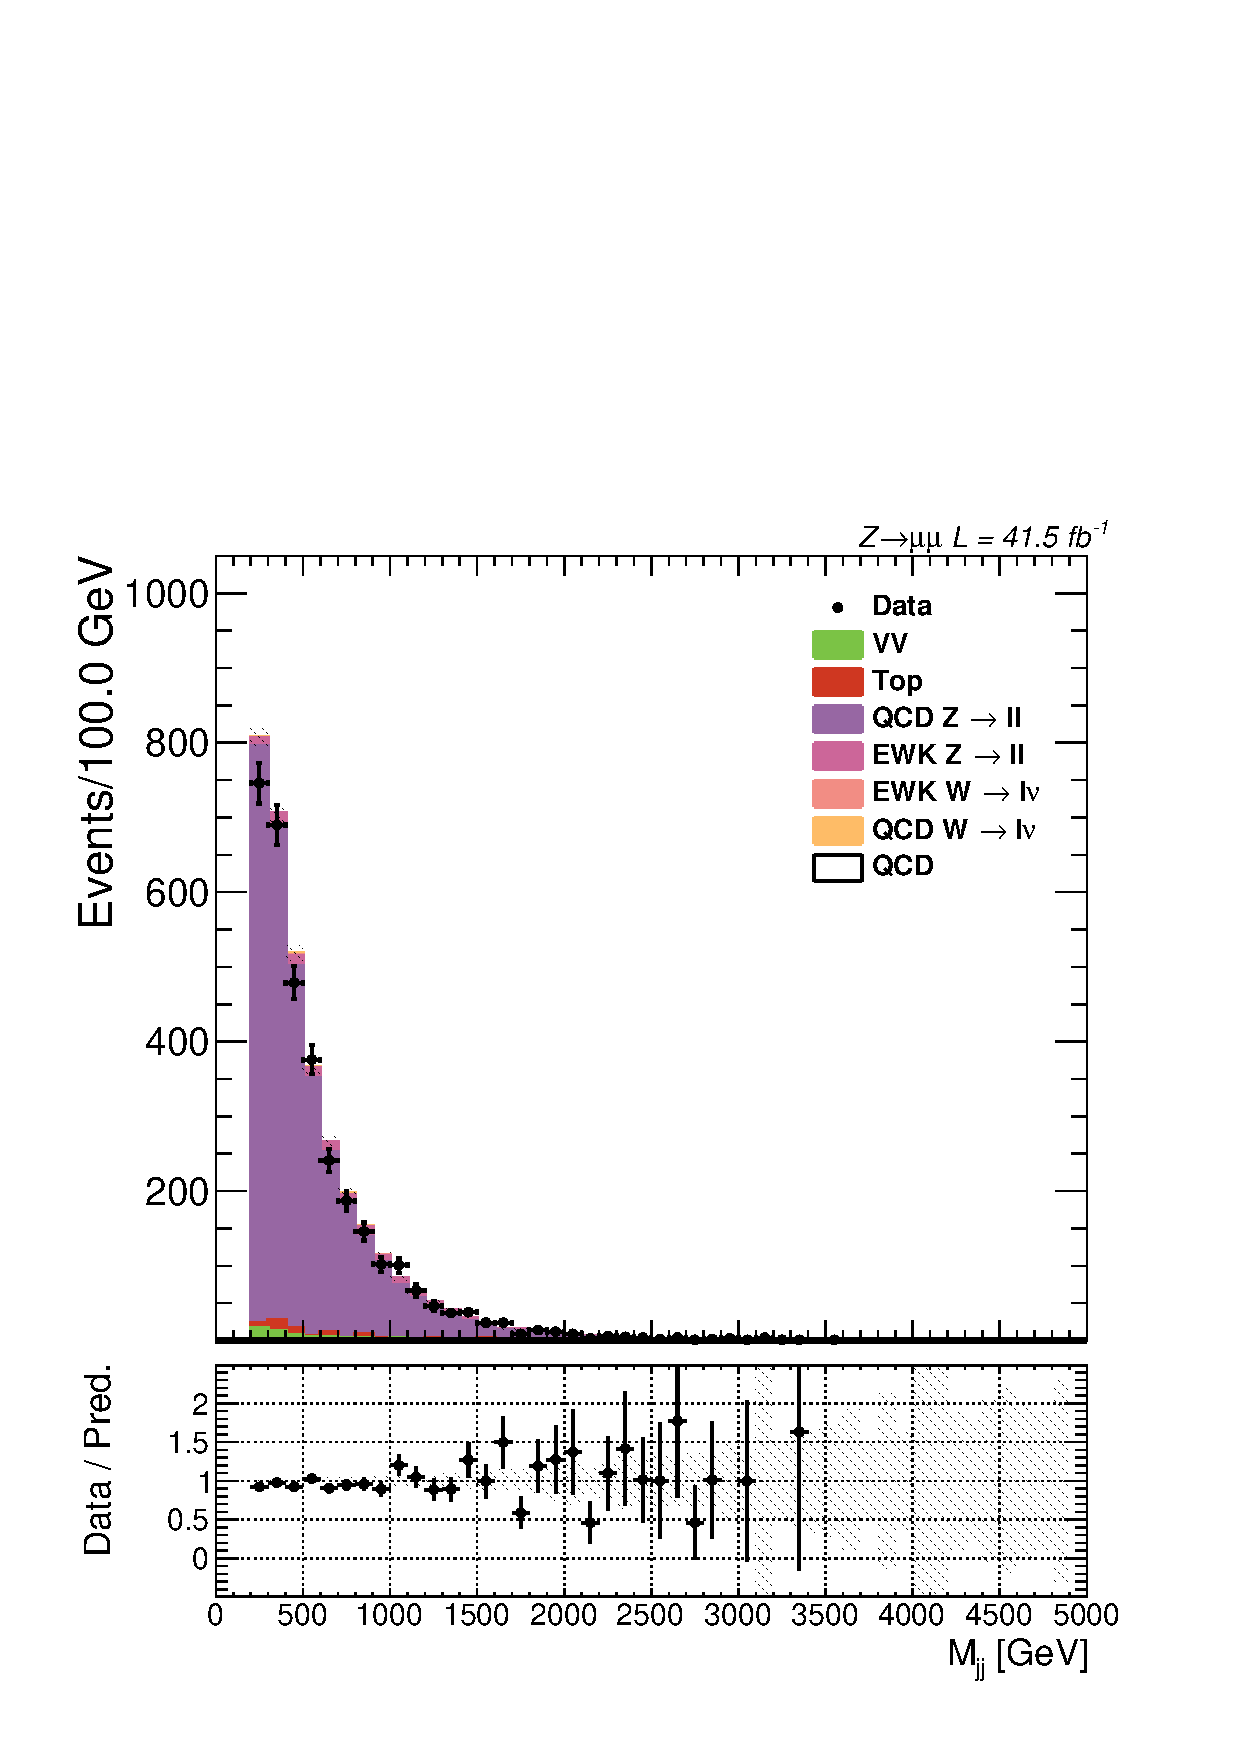
\includegraphics[width=0.49\textwidth]{Control_Regions/2017_MTR/Zmumu/leadingJet_mjj.pdf}
    }\\
    \subfigure[$m_{ll}$ - VTR]{
    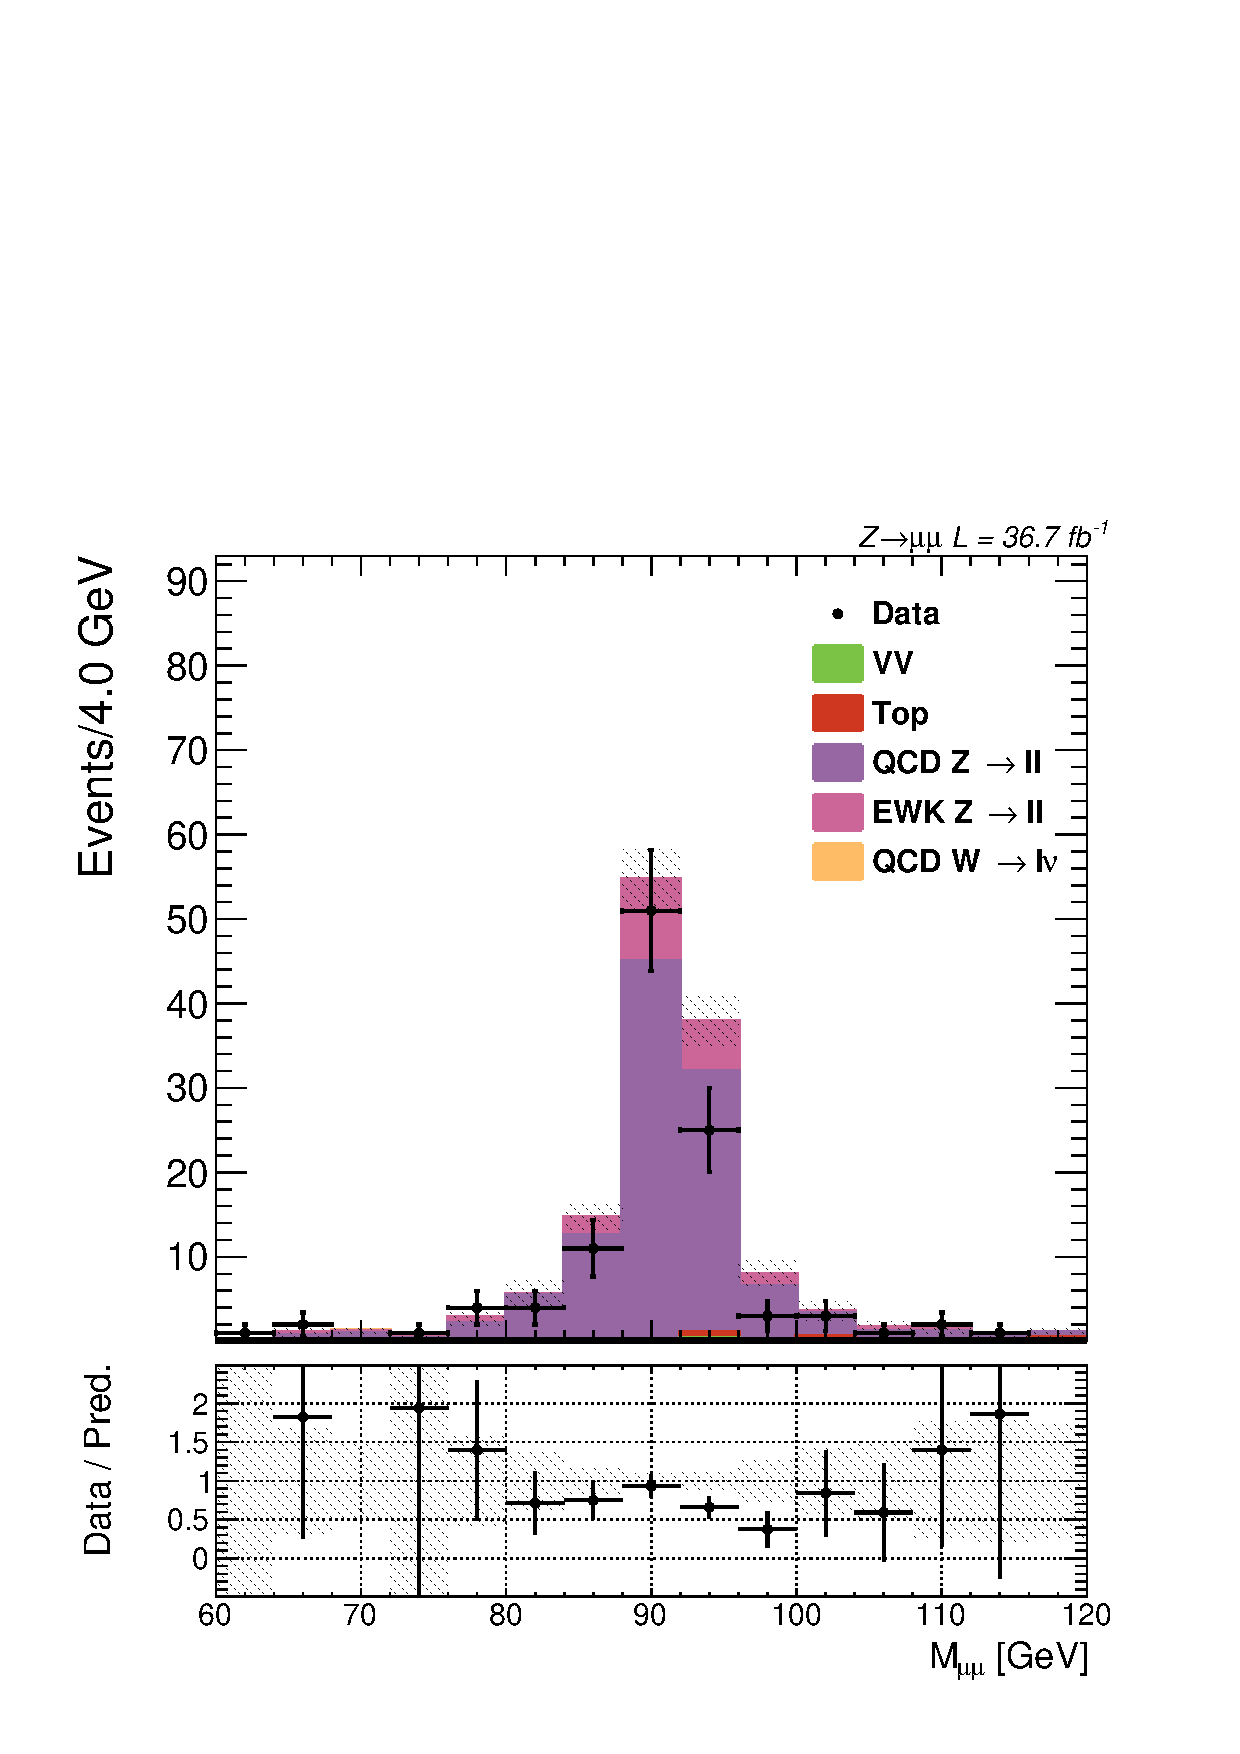
\includegraphics[width=0.49\textwidth]{Control_Regions/2017_VTR/Zmumu/diMuon_mass.pdf}
    }
    \subfigure[$m_{jj}$ - VTR]{
    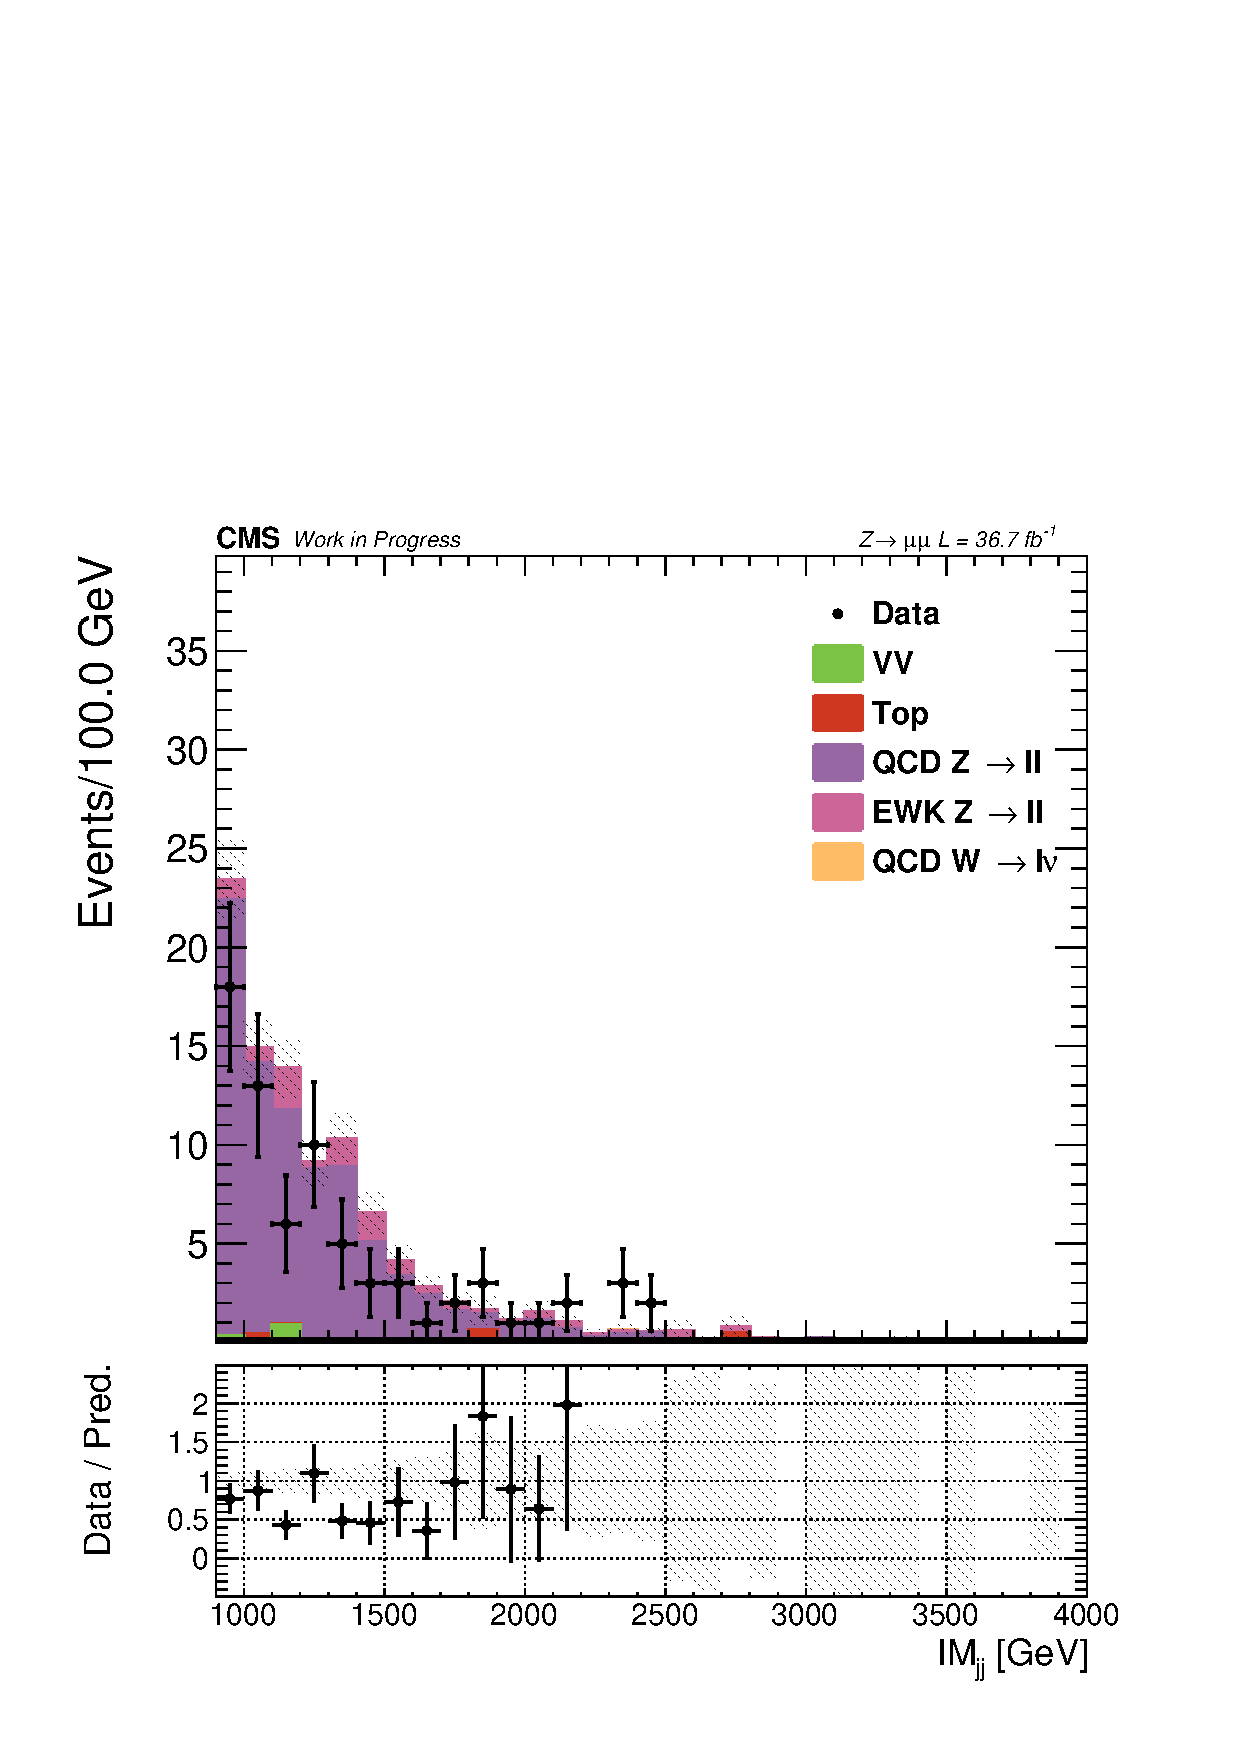
\includegraphics[width=0.49\textwidth]{Control_Regions/2017_VTR/Zmumu/lMjj.pdf}
    }
  \caption{Distributions of $m_{ll}$ and $m_{jj}$ variables in double muon region for MTR (top) and VTR (bottom) categories for the 2017 era of data taking.}
  \label{fig:2017_Zmumu_1}
\end{figure}

\begin{figure}[htbp]
  \centering
    \subfigure[$m_{ll}$ - MTR]{
    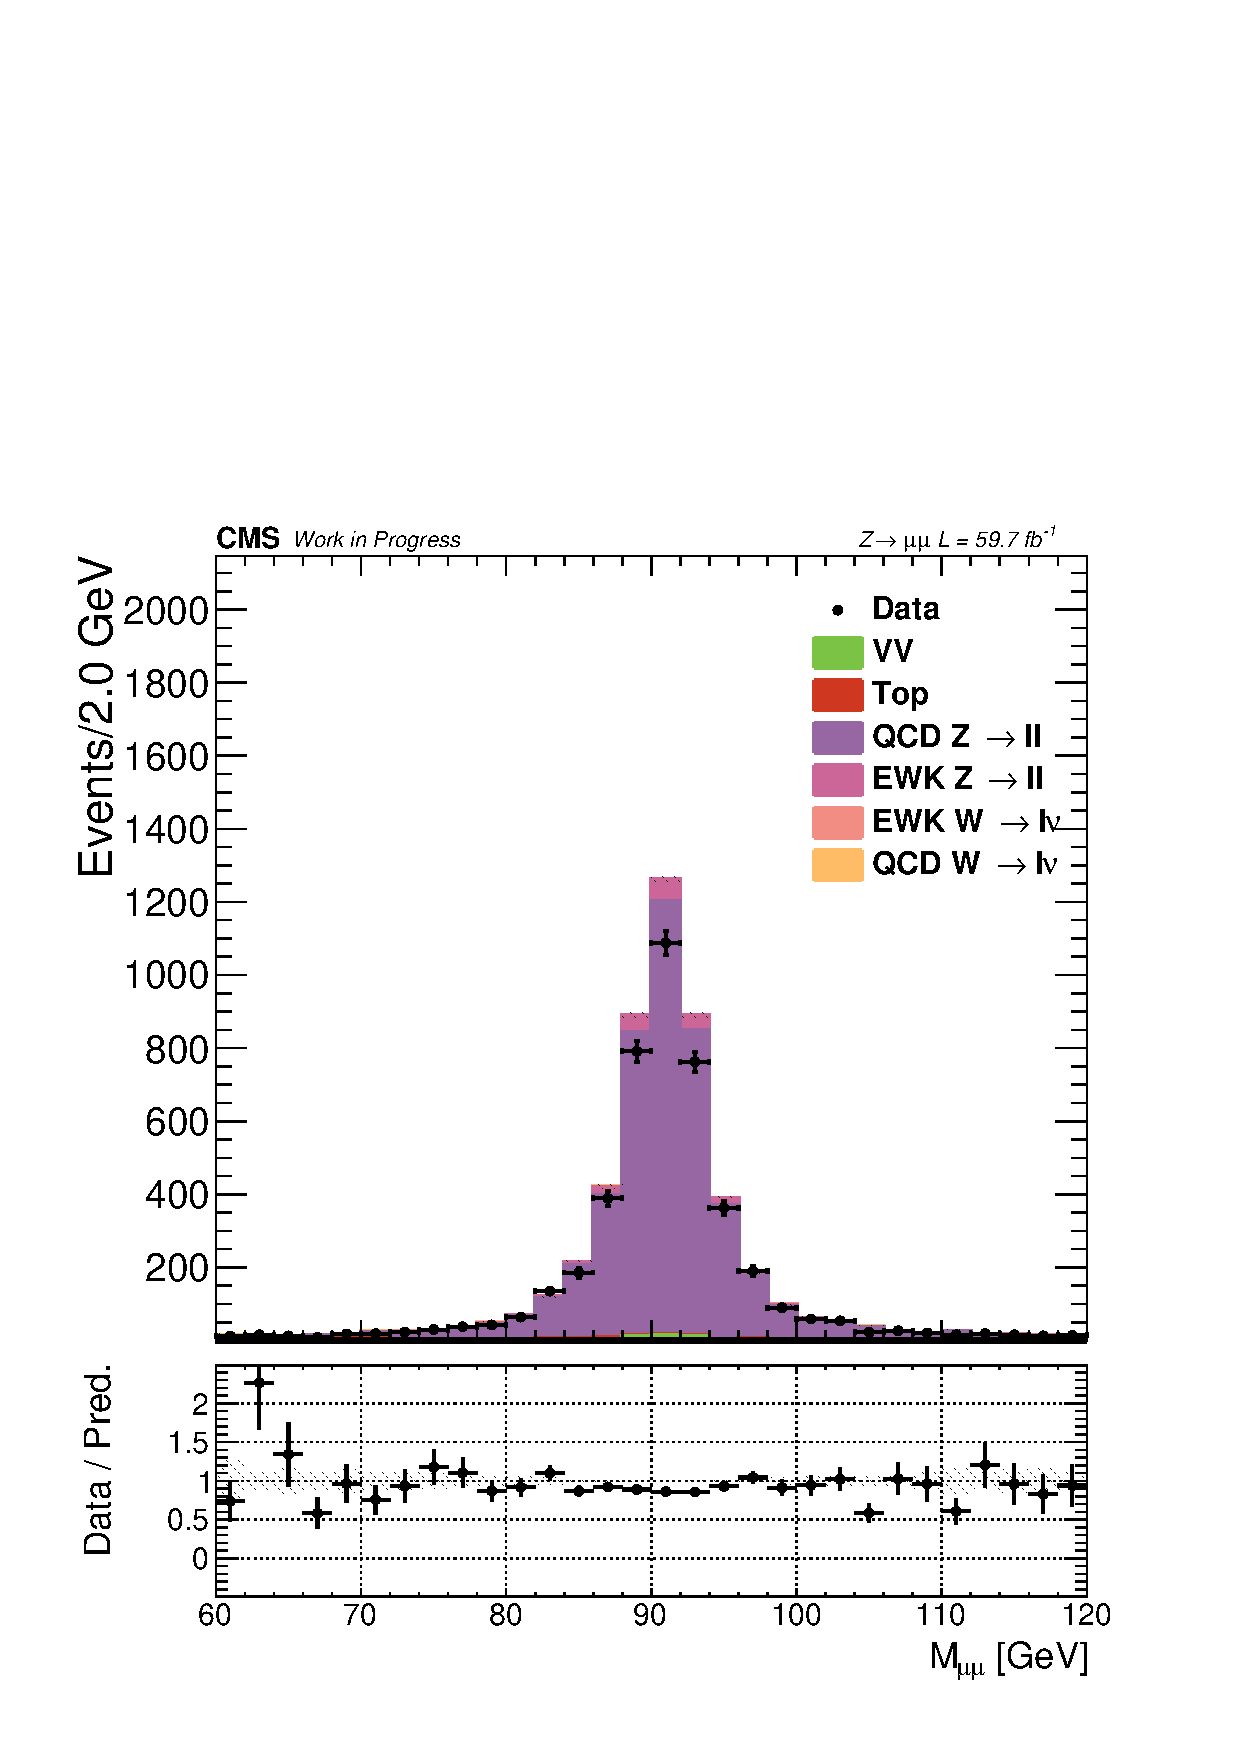
\includegraphics[width=0.49\textwidth]{Control_Regions/2018_MTR/Zmumu/diMuon_mass.pdf}
    }
    \subfigure[$m_{jj}$ - MTR]{
    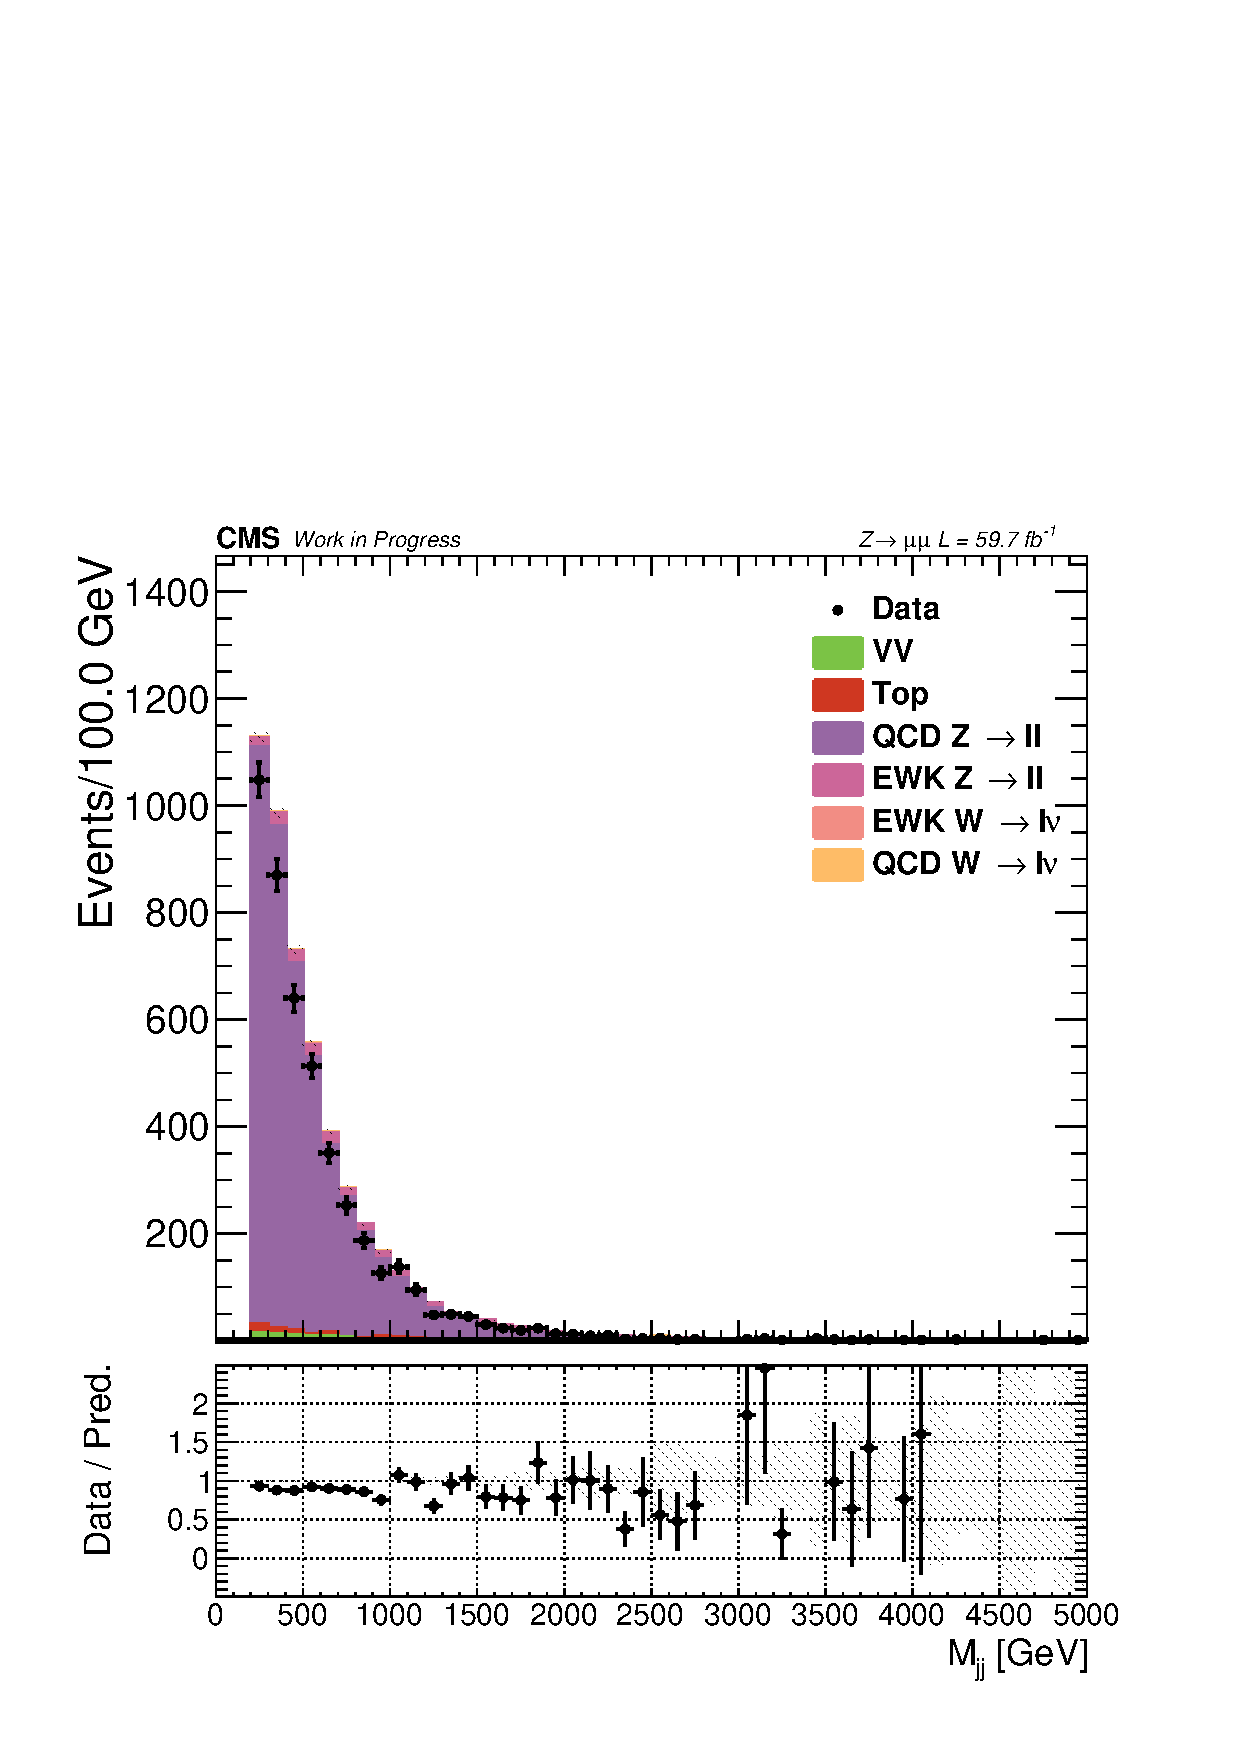
\includegraphics[width=0.49\textwidth]{Control_Regions/2018_MTR/Zmumu/leadingJet_mjj.pdf}
    }\\
    \subfigure[$m_{ll}$ - VTR]{
    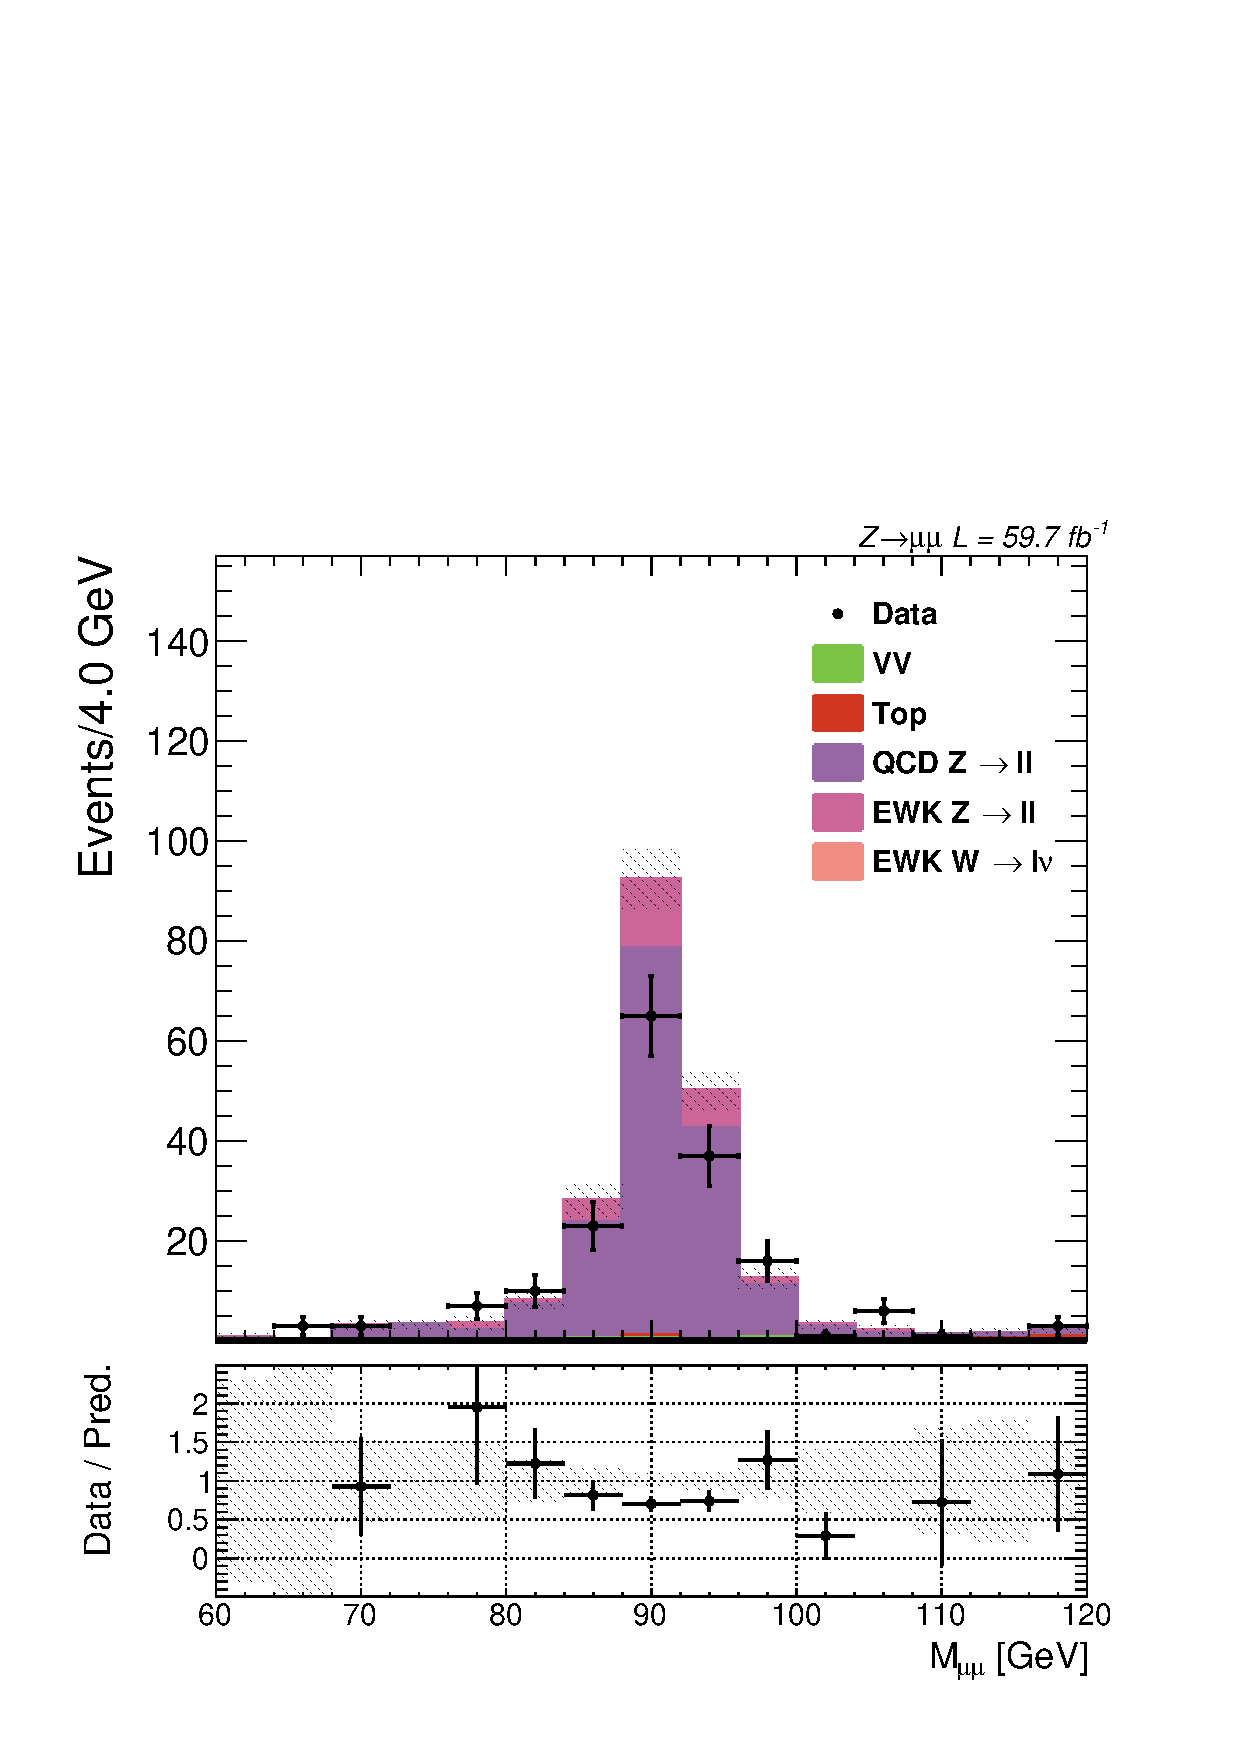
\includegraphics[width=0.49\textwidth]{Control_Regions/2018_VTR/Zmumu/diMuon_mass.pdf}
    }
    \subfigure[$m_{jj}$ - VTR]{
    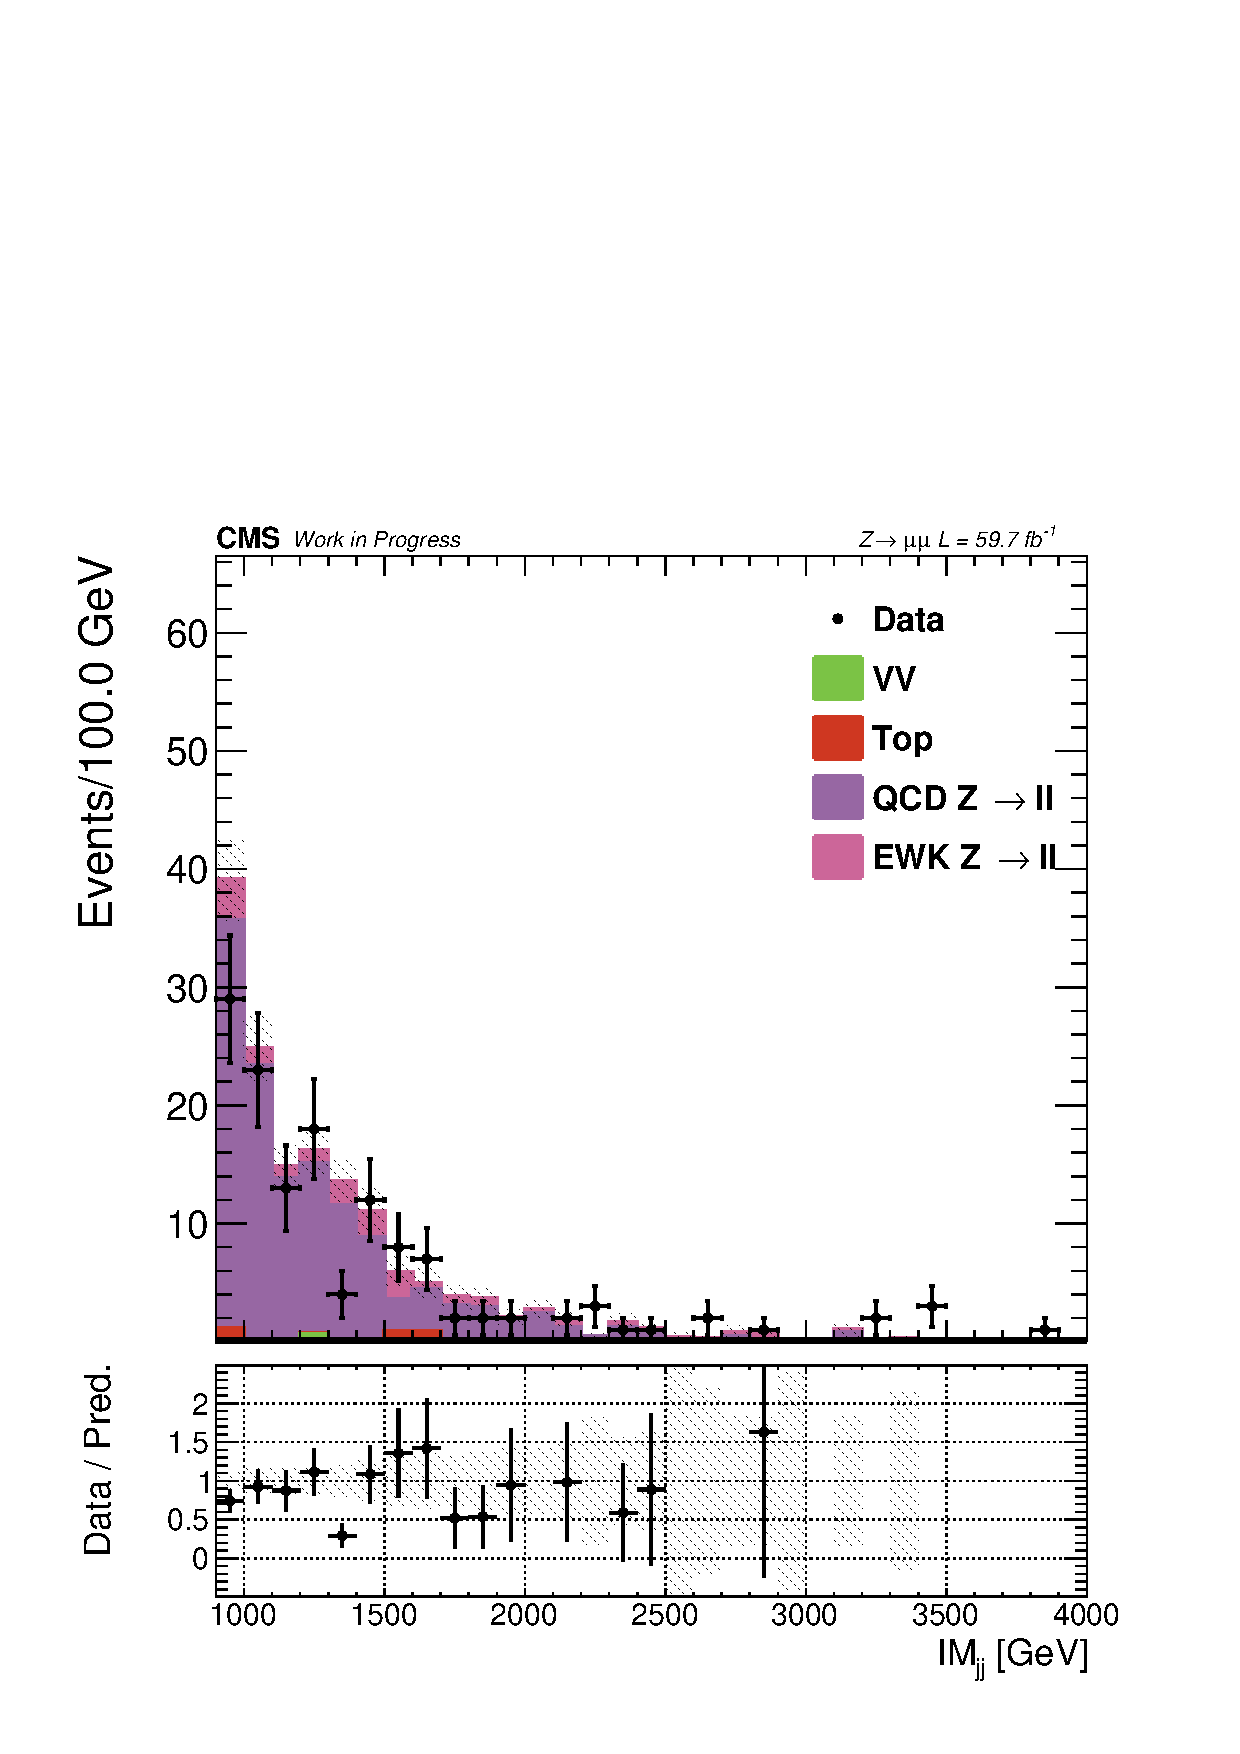
\includegraphics[width=0.49\textwidth]{Control_Regions/2018_VTR/Zmumu/lMjj.pdf}
    }
  \caption{Distributions of $m_{ll}$ and $m_{jj}$ variables in double muon region for MTR (top) and VTR (bottom) categories for the 2018 era of data taking.}
  \label{fig:2018_Zmumu_1}
\end{figure}


\begin{figure}[htbp]
  \centering
    \subfigure[$E_{T,miss}$ - MTR]{
    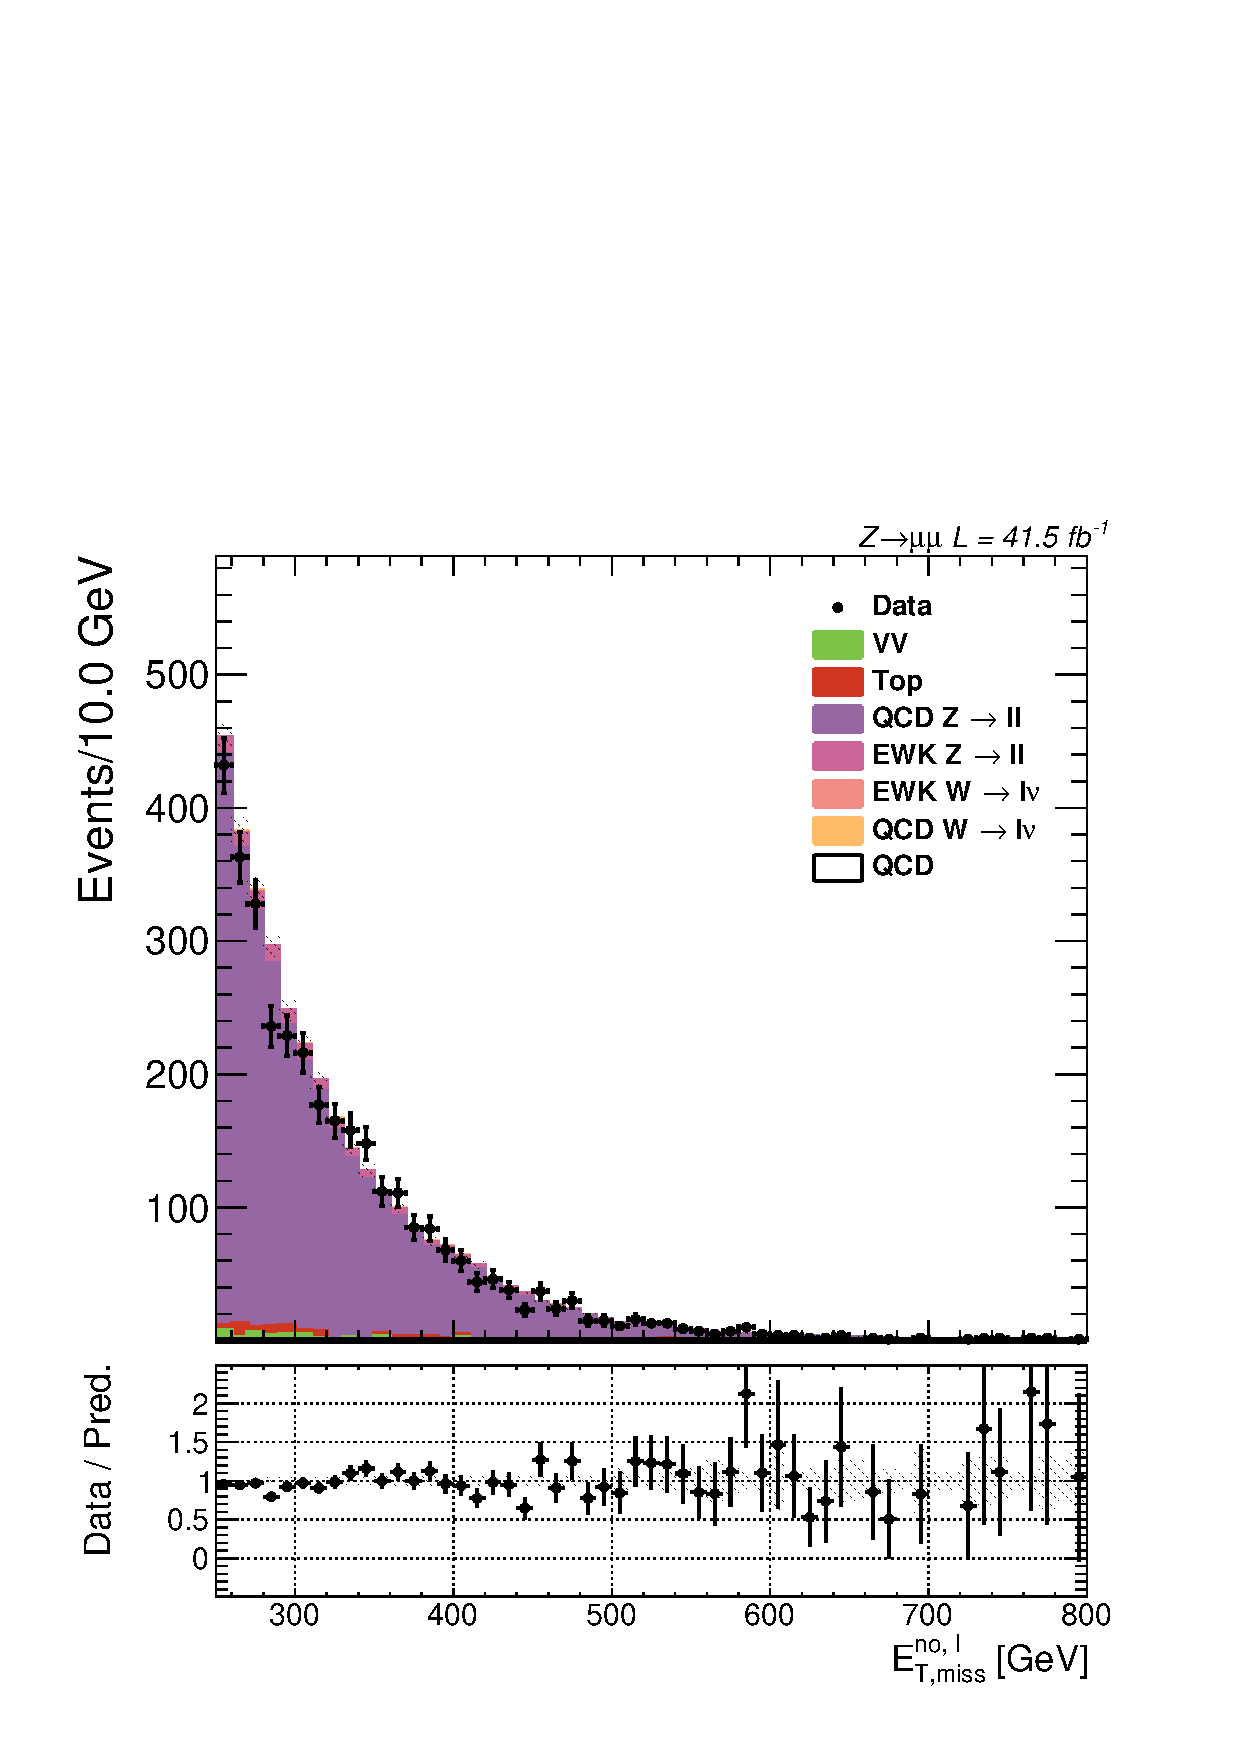
\includegraphics[width=0.49\textwidth]{Control_Regions/2017_MTR/Zmumu/MetNoMu.pdf}
    }
    \subfigure[$min\Delta\phi(j,E_{T,miss})$ - MTR]{
    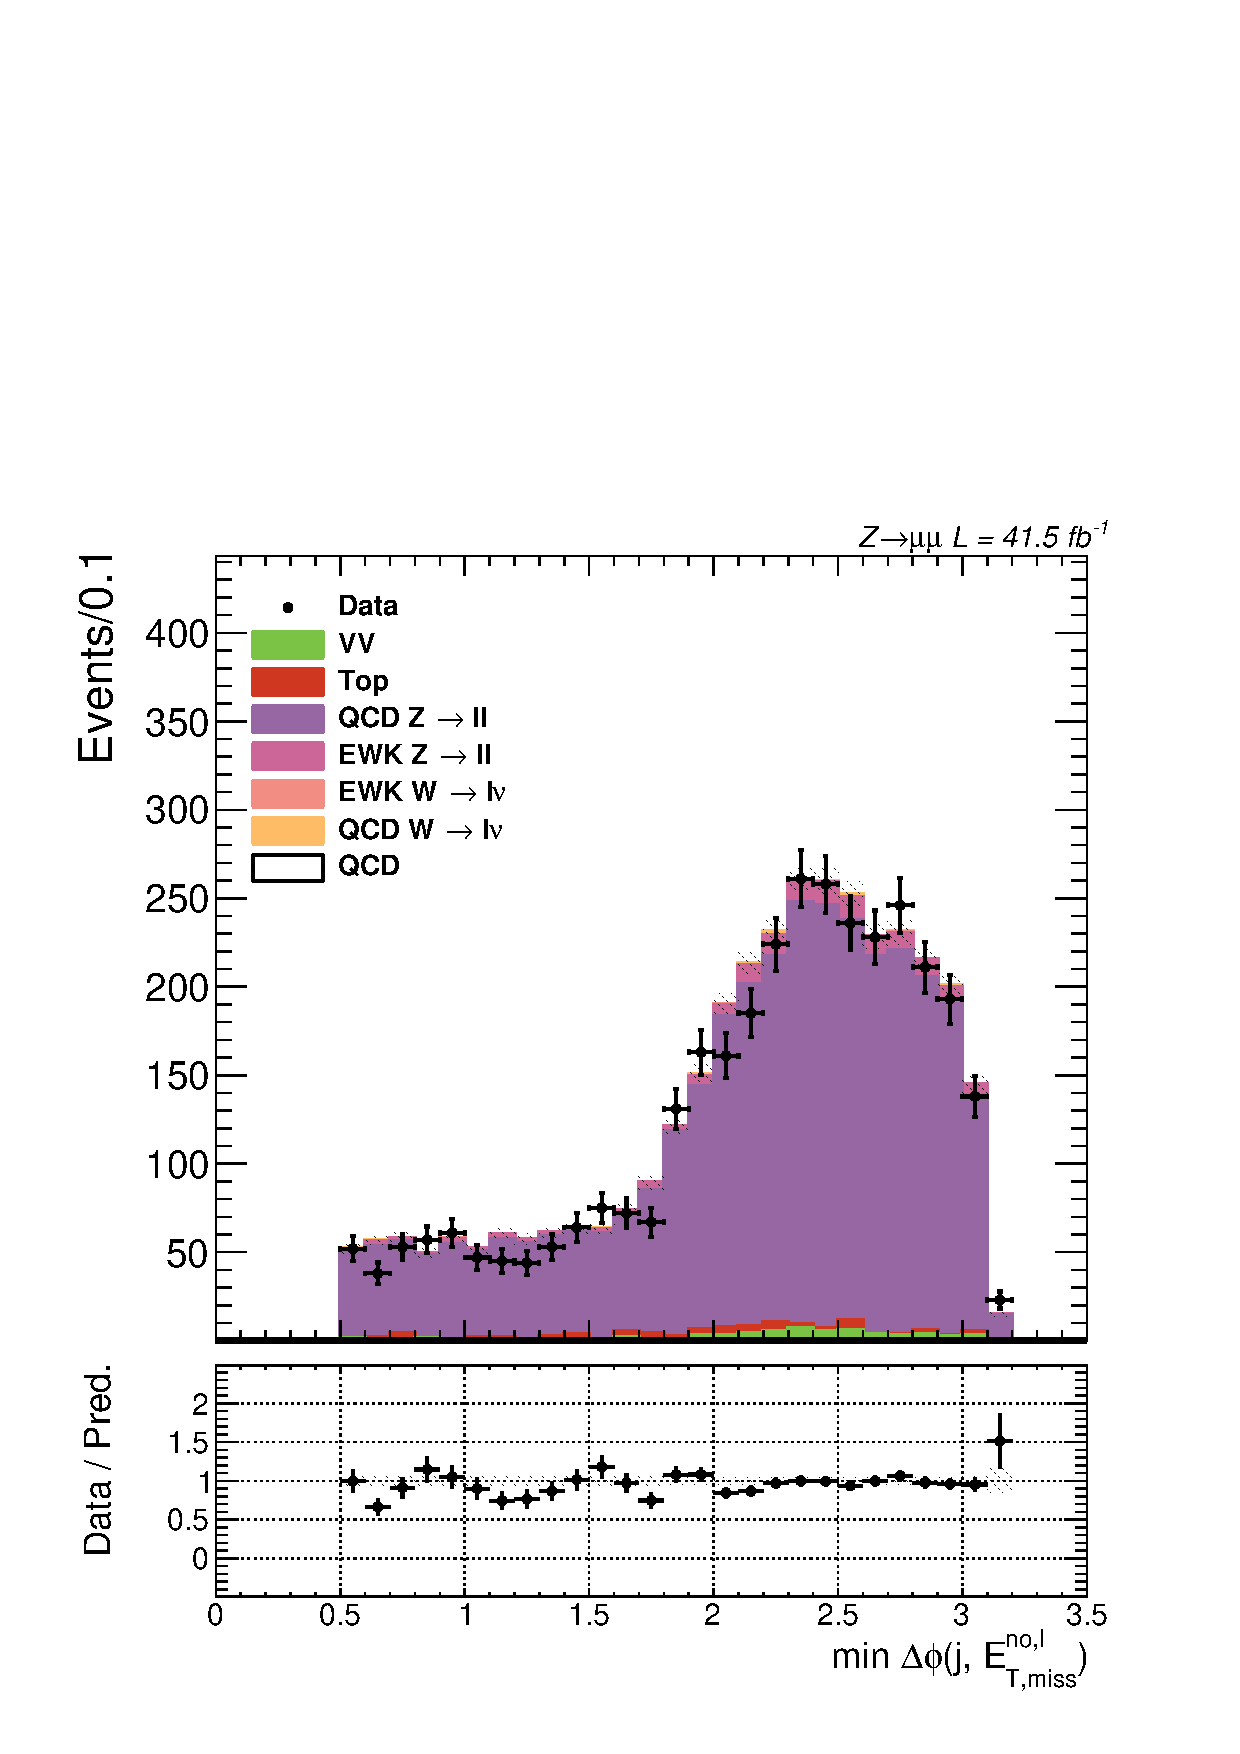
\includegraphics[width=0.49\textwidth]{Control_Regions/2017_MTR/Zmumu/MetNoLep_CleanJet_mindPhi.pdf}
    }\\
    \subfigure[$E_{T,miss}$ - VTR]{
    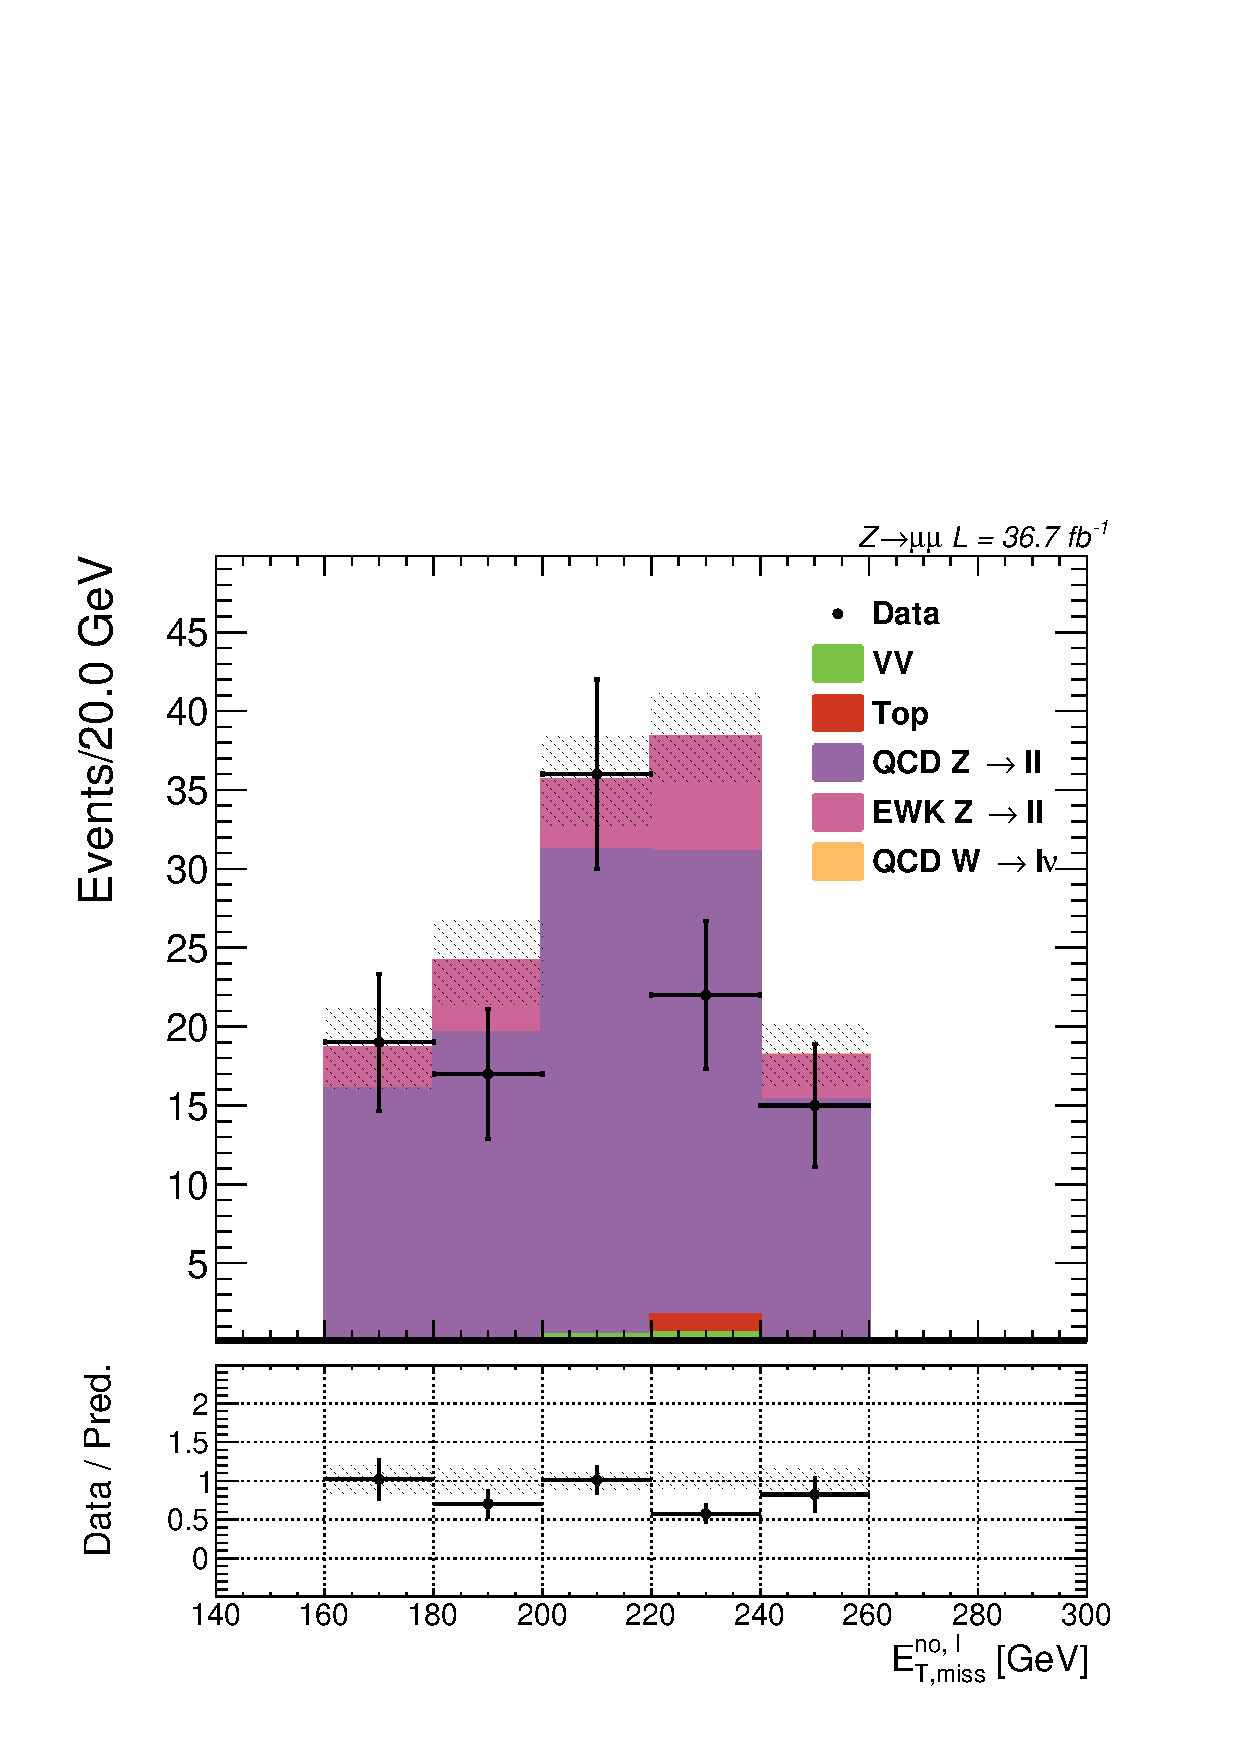
\includegraphics[width=0.49\textwidth]{Control_Regions/2017_VTR/Zmumu/MetNoMu.pdf}
    }
    \subfigure[$min\Delta\phi(j,E_{T,miss})$ - VTR]{
    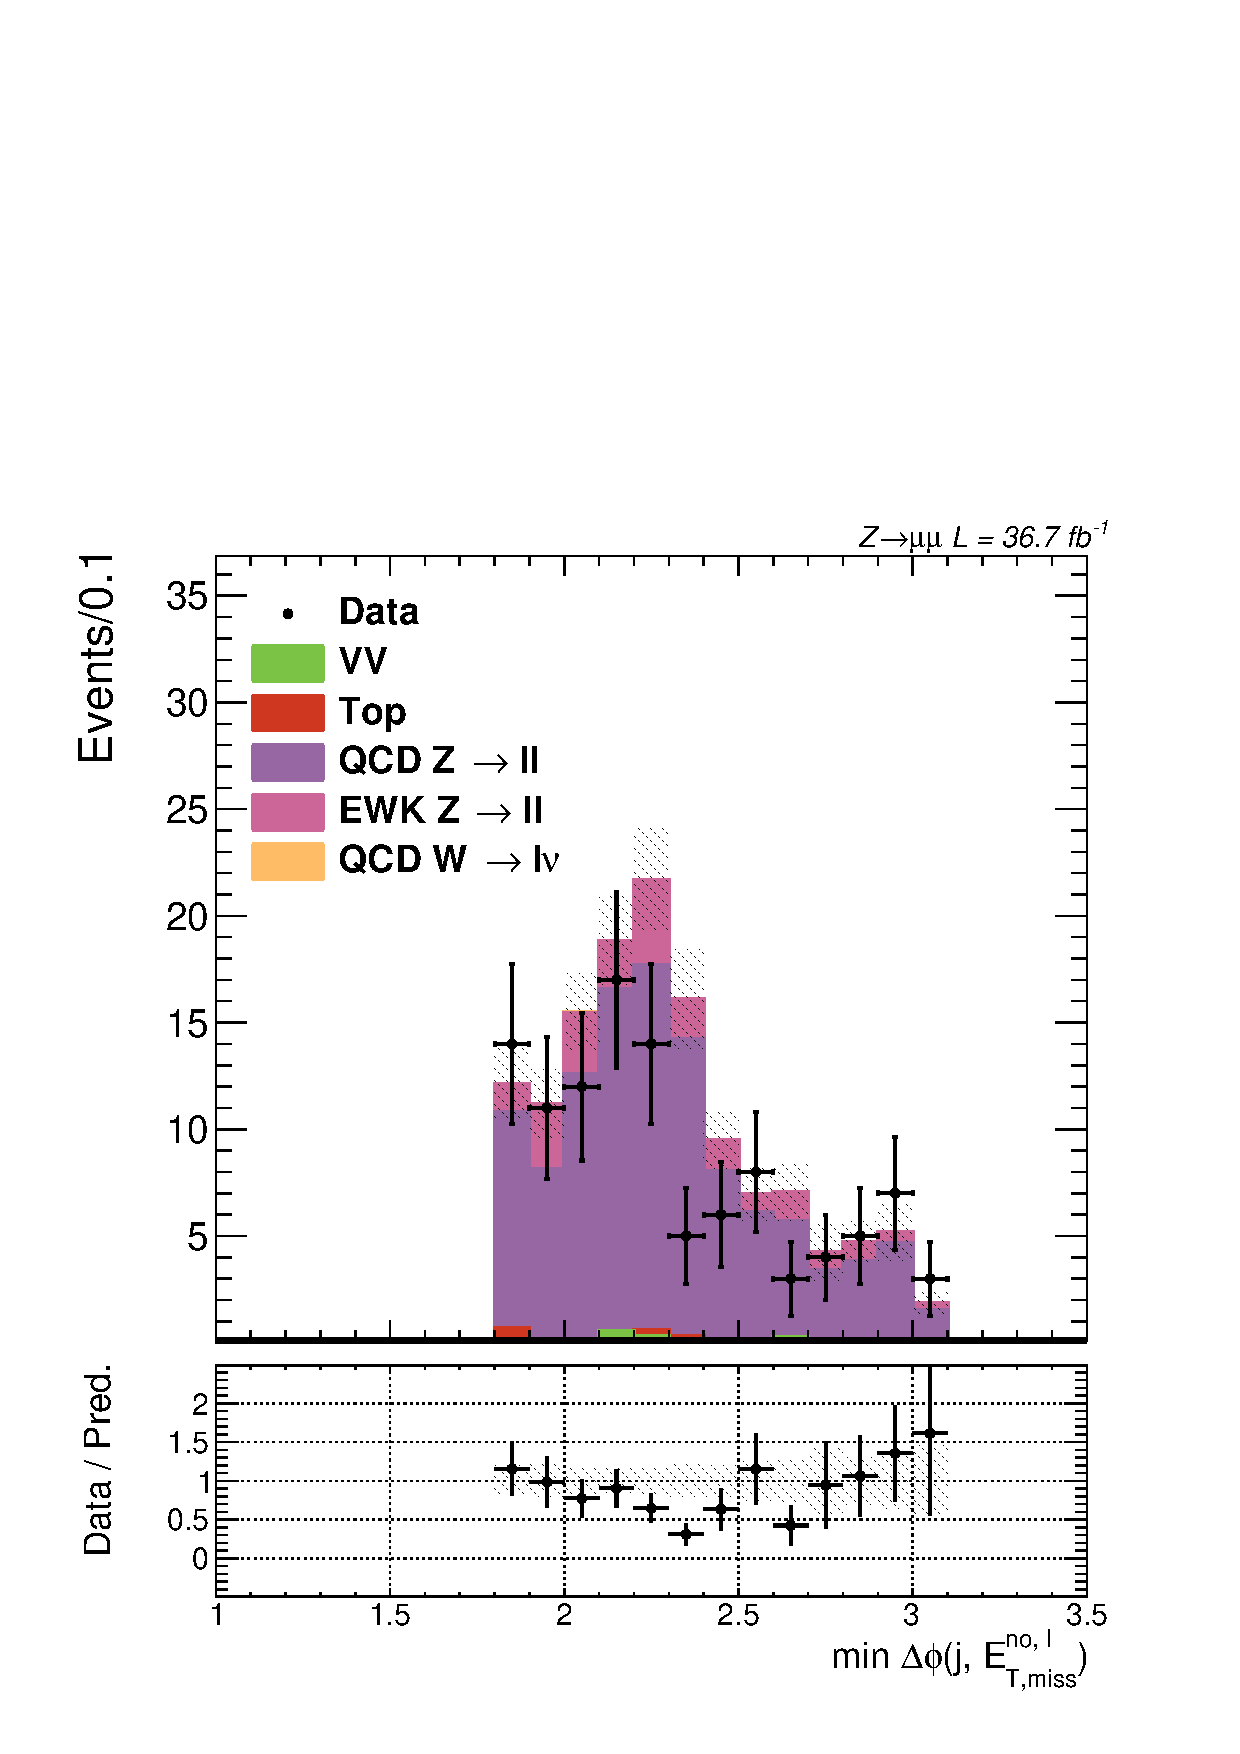
\includegraphics[width=0.49\textwidth]{Control_Regions/2017_VTR/Zmumu/MetNoLep_CleanJet_mindPhi.pdf}
    }
  \caption{Distributions of the $E_{T,miss}$ and $min\Delta\phi(j,E_{T,miss})$  variables in double muon region for MTR (top) and VTR (bottom) categories for the 2017 era of data taking.}
  \label{fig:2017_Zmumu_2}
\end{figure}


\begin{figure}[htbp]
  \centering
    \subfigure[$E_{T,miss}$ - MTR]{
    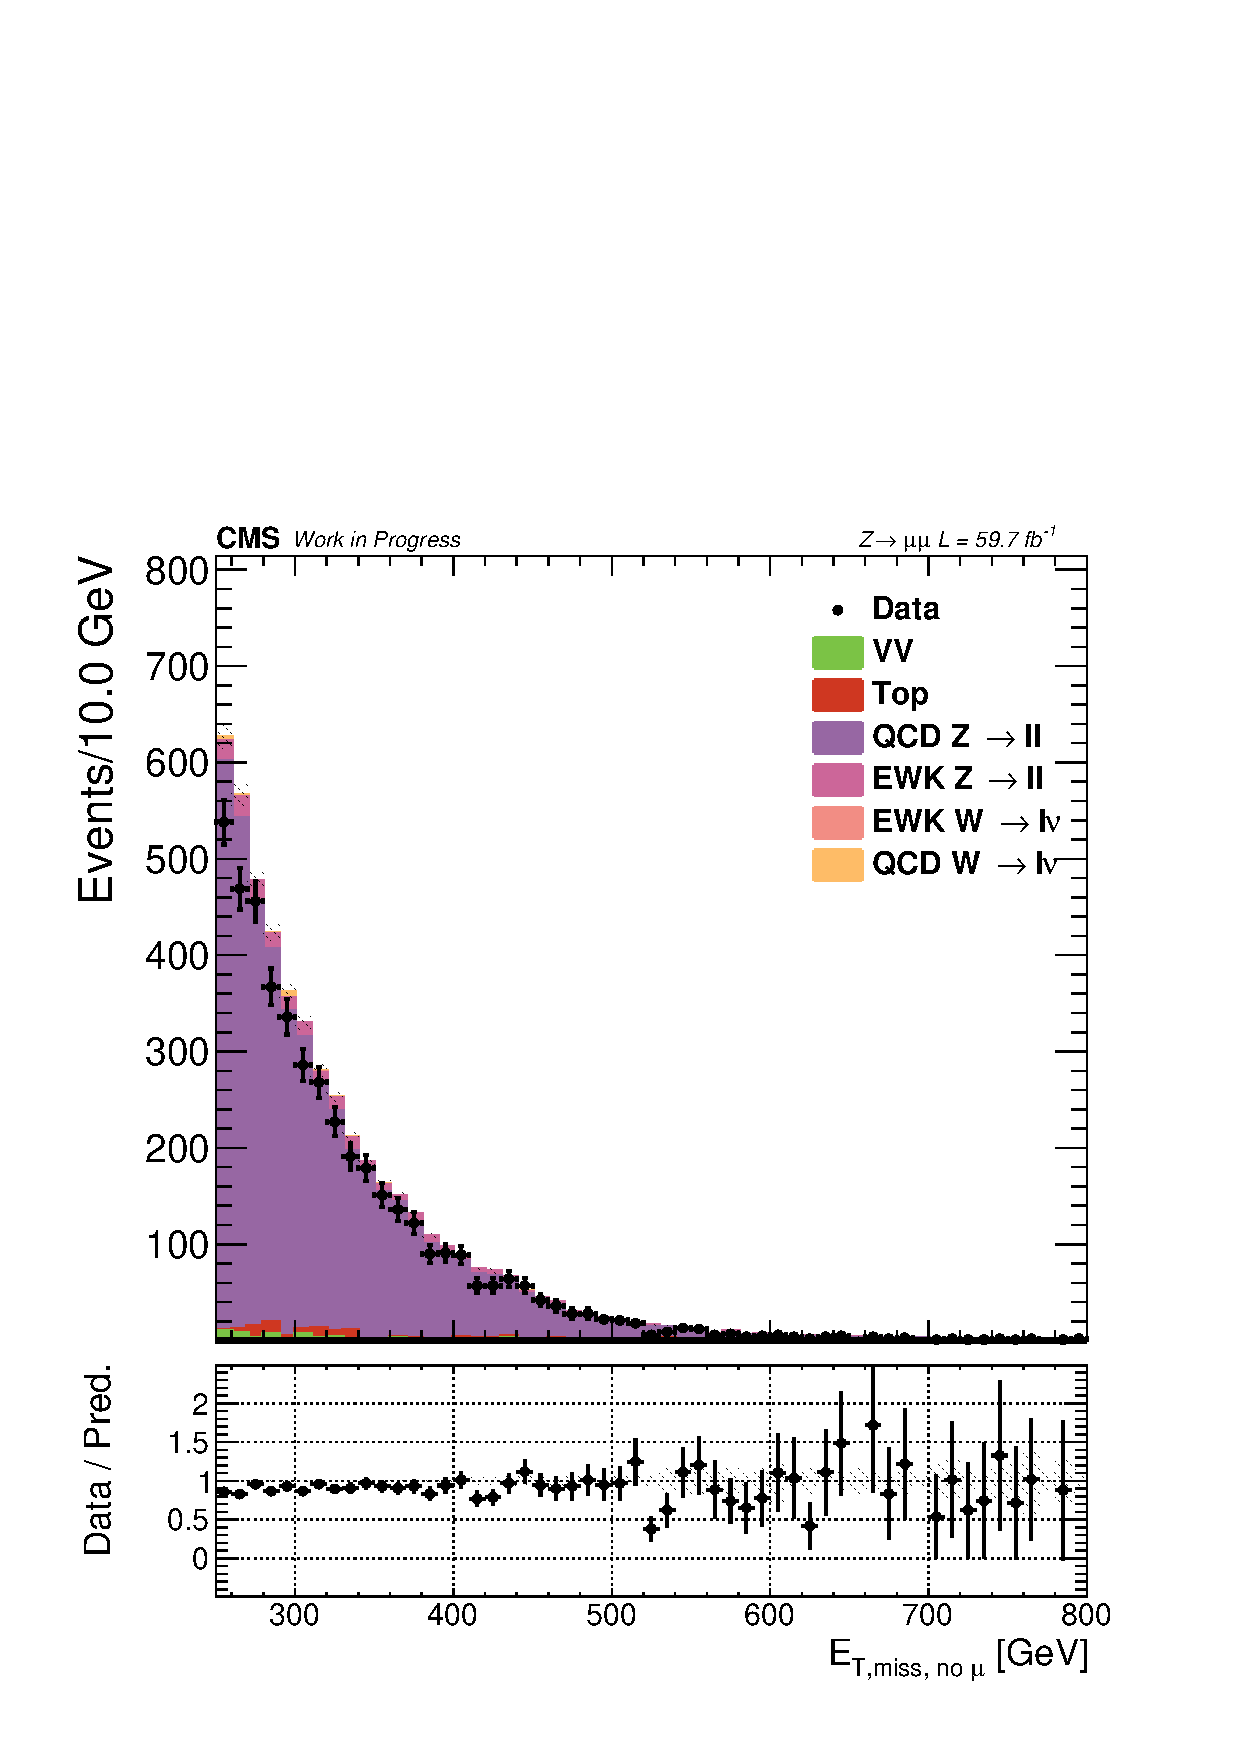
\includegraphics[width=0.49\textwidth]{Control_Regions/2018_MTR/Zmumu/MetNoMu.pdf}
    }
    \subfigure[$min\Delta\phi(j,E_{T,miss})$ - MTR]{
    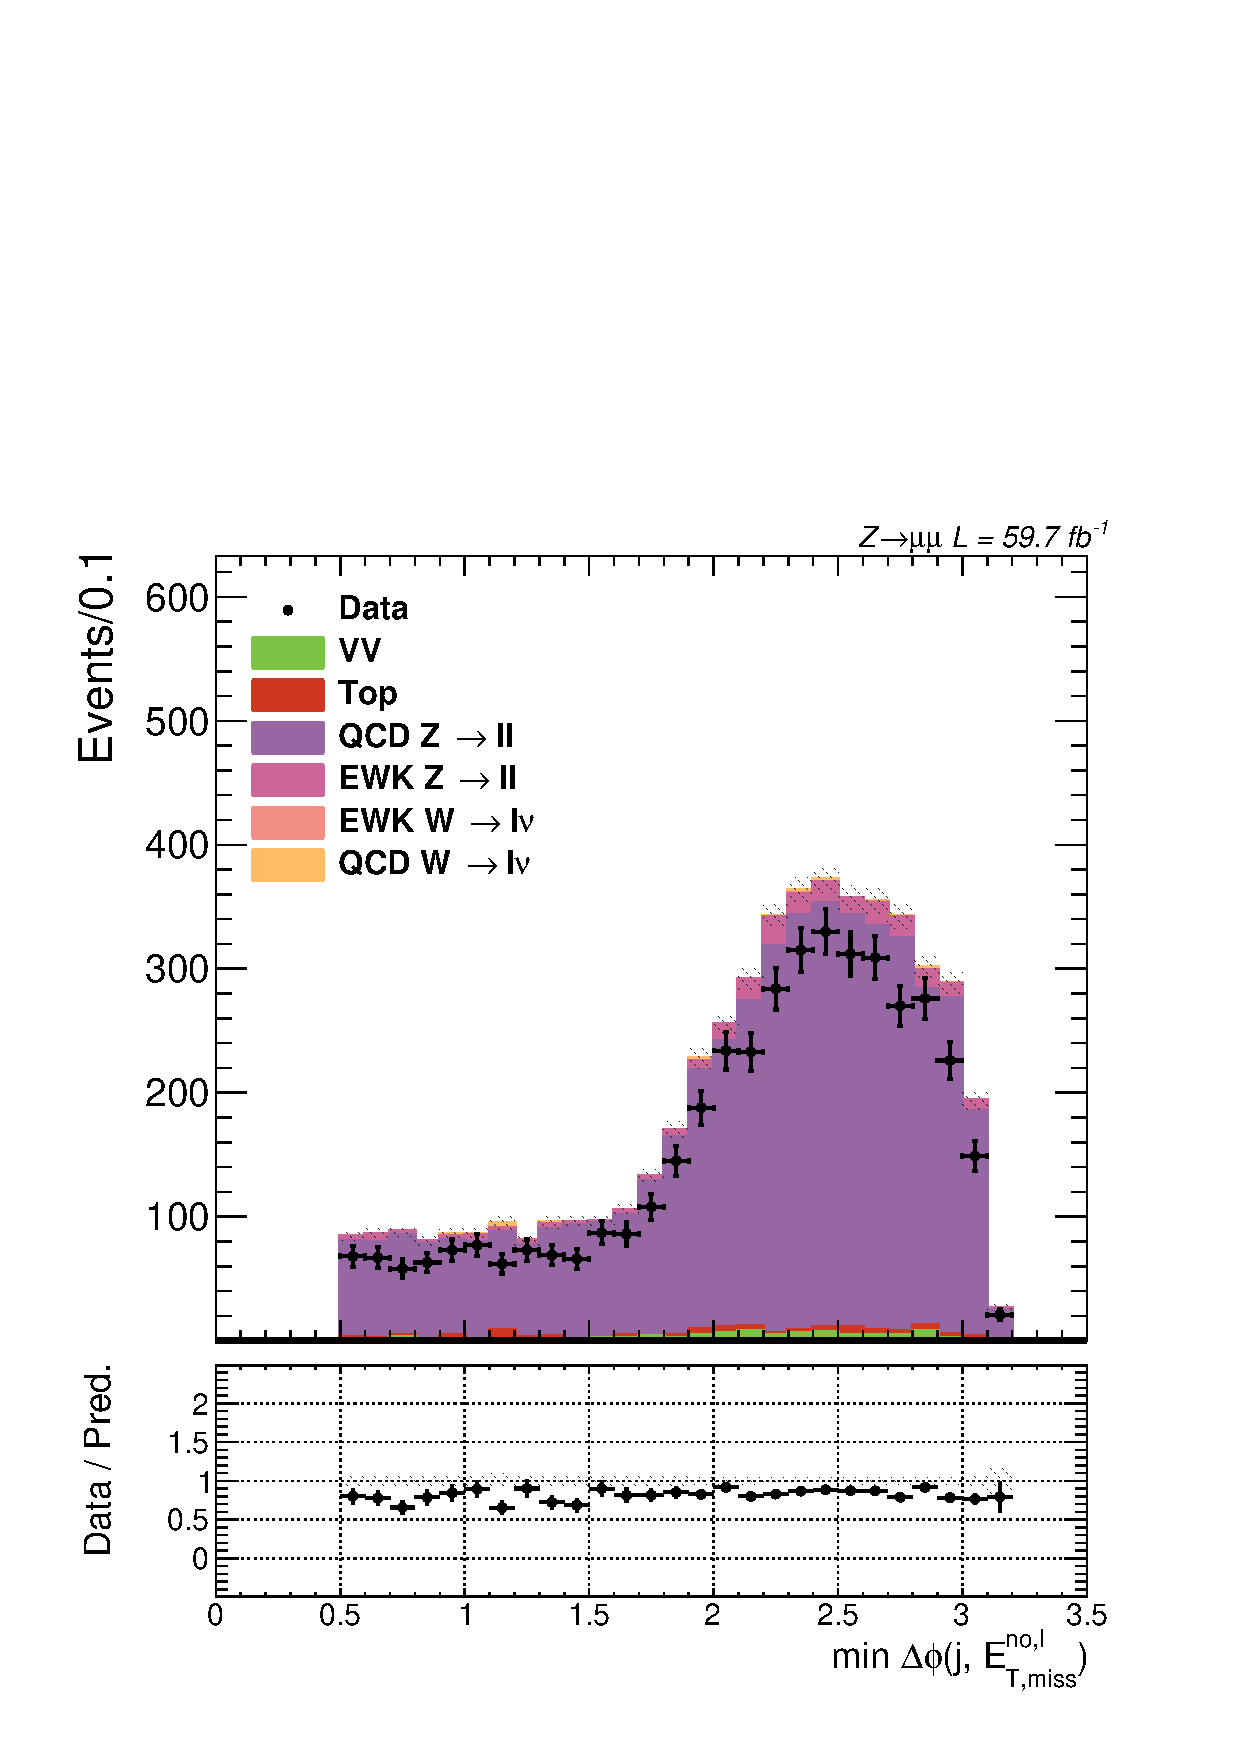
\includegraphics[width=0.49\textwidth]{Control_Regions/2018_MTR/Zmumu/MetNoLep_CleanJet_mindPhi.pdf}
    }\\
    \subfigure[$E_{T,miss}$ - VTR]{
    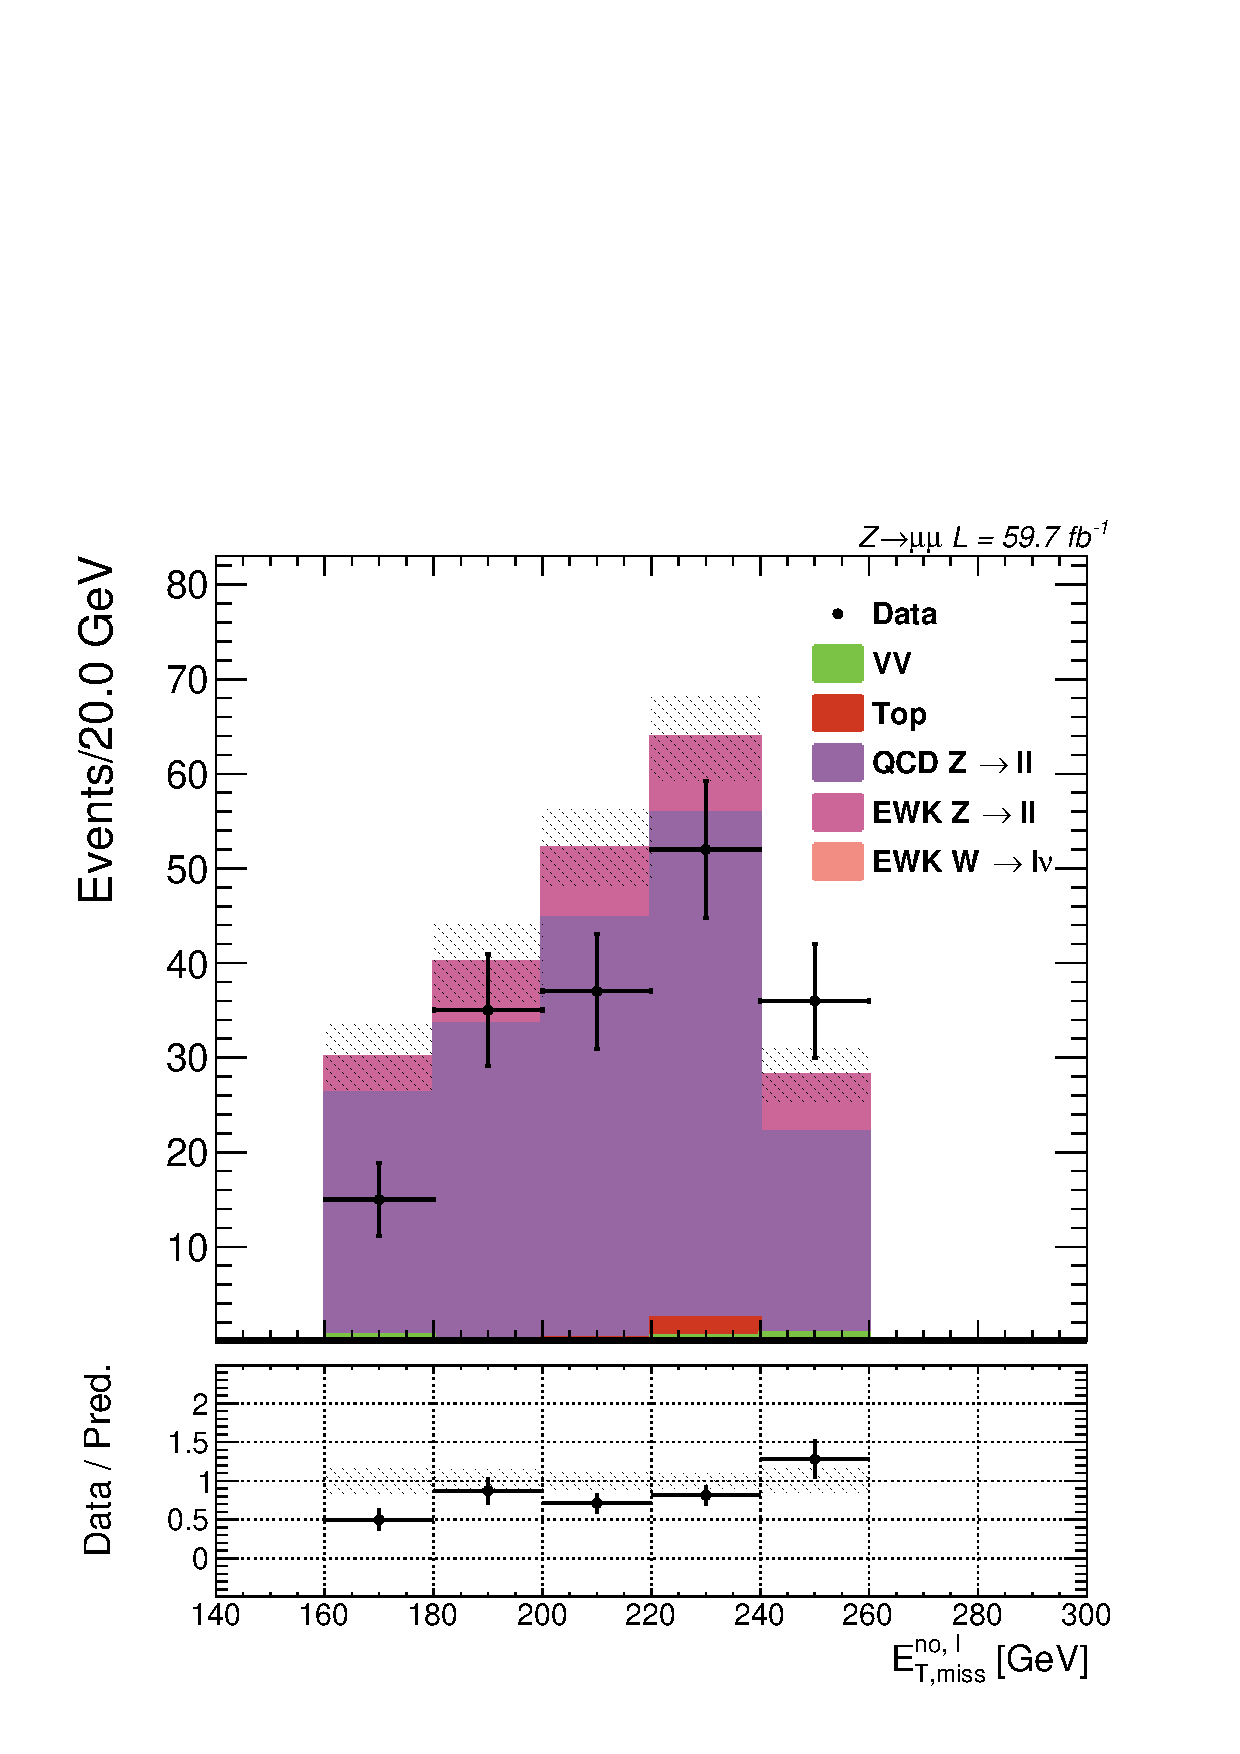
\includegraphics[width=0.49\textwidth]{Control_Regions/2018_VTR/Zmumu/MetNoMu.pdf}
    }
    \subfigure[$min\Delta\phi(j,E_{T,miss})$ - VTR]{
    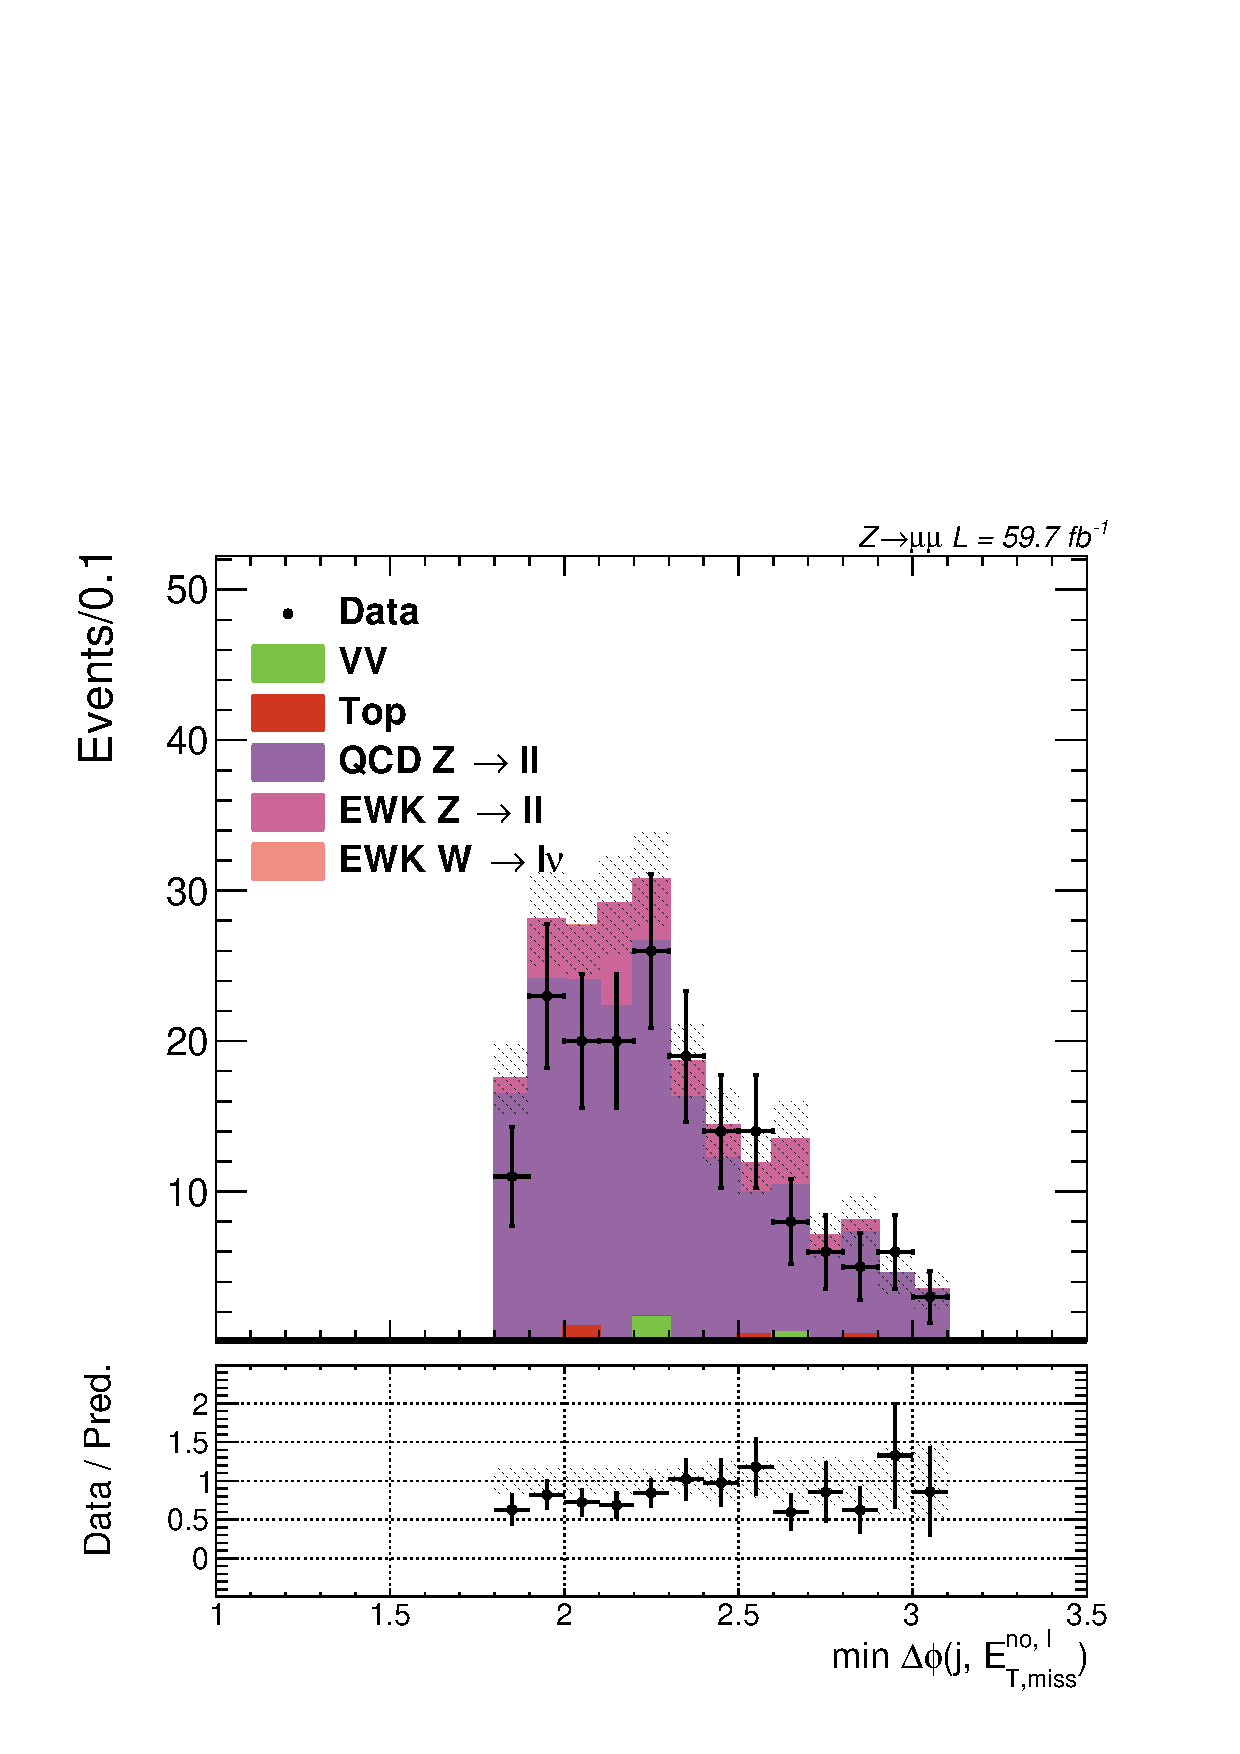
\includegraphics[width=0.49\textwidth]{Control_Regions/2018_VTR/Zmumu/MetNoLep_CleanJet_mindPhi.pdf}
    }
  \caption{Distributions of the $E_{T,miss}$ and $min\Delta\phi(j,E_{T,miss})$ variables in double muon region for MTR (top) and VTR (bottom) categories for the 2018 era of data taking.}
  \label{fig:2018_Zmumu_2}
\end{figure}
\hspace{10pt} This is evident in 2018, where there is a complete absence of any excess originating from the HEM problem, which can be tested by taking a look at $\phi$ variables for $\vec{p}_{T, miss}$ and the leading jet (shown in Figure~\ref{fig:Zmumu_noHEM} for the MTR category). The influence of QCD multijet processes has also been diminished by these conditions for both eras. Additional distributions showing leading and subleading muon properties as well as more detailed jet information are presented in Appendix~\ref{app:CRs}.

\subsection{Single Muon CR}
\label{sec:single_muon}
\hspace{10pt} Continuing with the muon structures, the next item is the single muon region. Formed from VBF-like events, similarly to double muon regions, by modifying the muon veto requirement for both MTR/VTR selections. The new requirement states that the event needs to contain exactly one muon with $p_T>$~20~GeV, which also satisfies tight muon requirements.

\hspace{10pt} Figures~\ref{fig:2017_Wmunu_1} and~\ref{fig:2018_Wmunu_1} show distributions of the $m_{jj}$ and $E_{T,miss}^{no~\mu}$ in this region for both categories and both eras. The data to prediction agreement for the main variable considered in the fit is very good for the low $m_{jj}$ bins, with the disagreement in the higher bins being significantly reduced with a choice of wider bins when performing the fit (more details about the fit procedure are given in Chapter~\ref{ch:fit}).

\hspace{10pt} For these single lepton regions, a new variable of interest is introduced. The transverse mass of a two object system is defined as:
\begin{equation}
    M_T= \sqrt{m_1^2+m_2^2+2\cdot(E_{T_1}E_{T_2}-\vec{p}_{T_1}\vec{p}_{T_2})},
\end{equation}
where the $m_i$, $E_{T,i}$ and $p_{T_i}$ denote the mass, the transverse energy and the transverse momentum of a physics object. For the scenarios where $m_i\rightarrow$~0, the previous formula can be rewritten using the following approximation:
\begin{equation}
    M_T= \sqrt{2\cdot(E_{T_1}E_{T_2}(1-cos\theta))},
\end{equation}
where $\theta$ represents the angle between two transverse momentum vectors. For the purposes of this region, two physics objects considered in the aforementioned calculation are going to be the $\vec{p}_{T, miss}$ and the transverse momentum of the selected muon. In the past, this variable (in further text referred to as $M_{T, \mu}$) was proved useful for the control of the contribution originating from the QCD multijet processes. Presented alongside the \mindphinomu variable in Figures~\ref{fig:2017_Wmunu_2} and~\ref{fig:2018_Wmunu_2}, for 2017 and 2018 eras respectively, it indicates a good agreement between data and simulation and significantly reduced QCD multijet contribution (requiring no additional requirement for this region).


%It was previously used as an additional selection requirement of $M_{T, \mu}<$~160~GeV in order to remove the data to simulation discrepancy seen in the high $M_T$ region. 


\begin{figure}[htbp]
  \centering
    \subfigure[$m_{jj}$ - MTR]{
    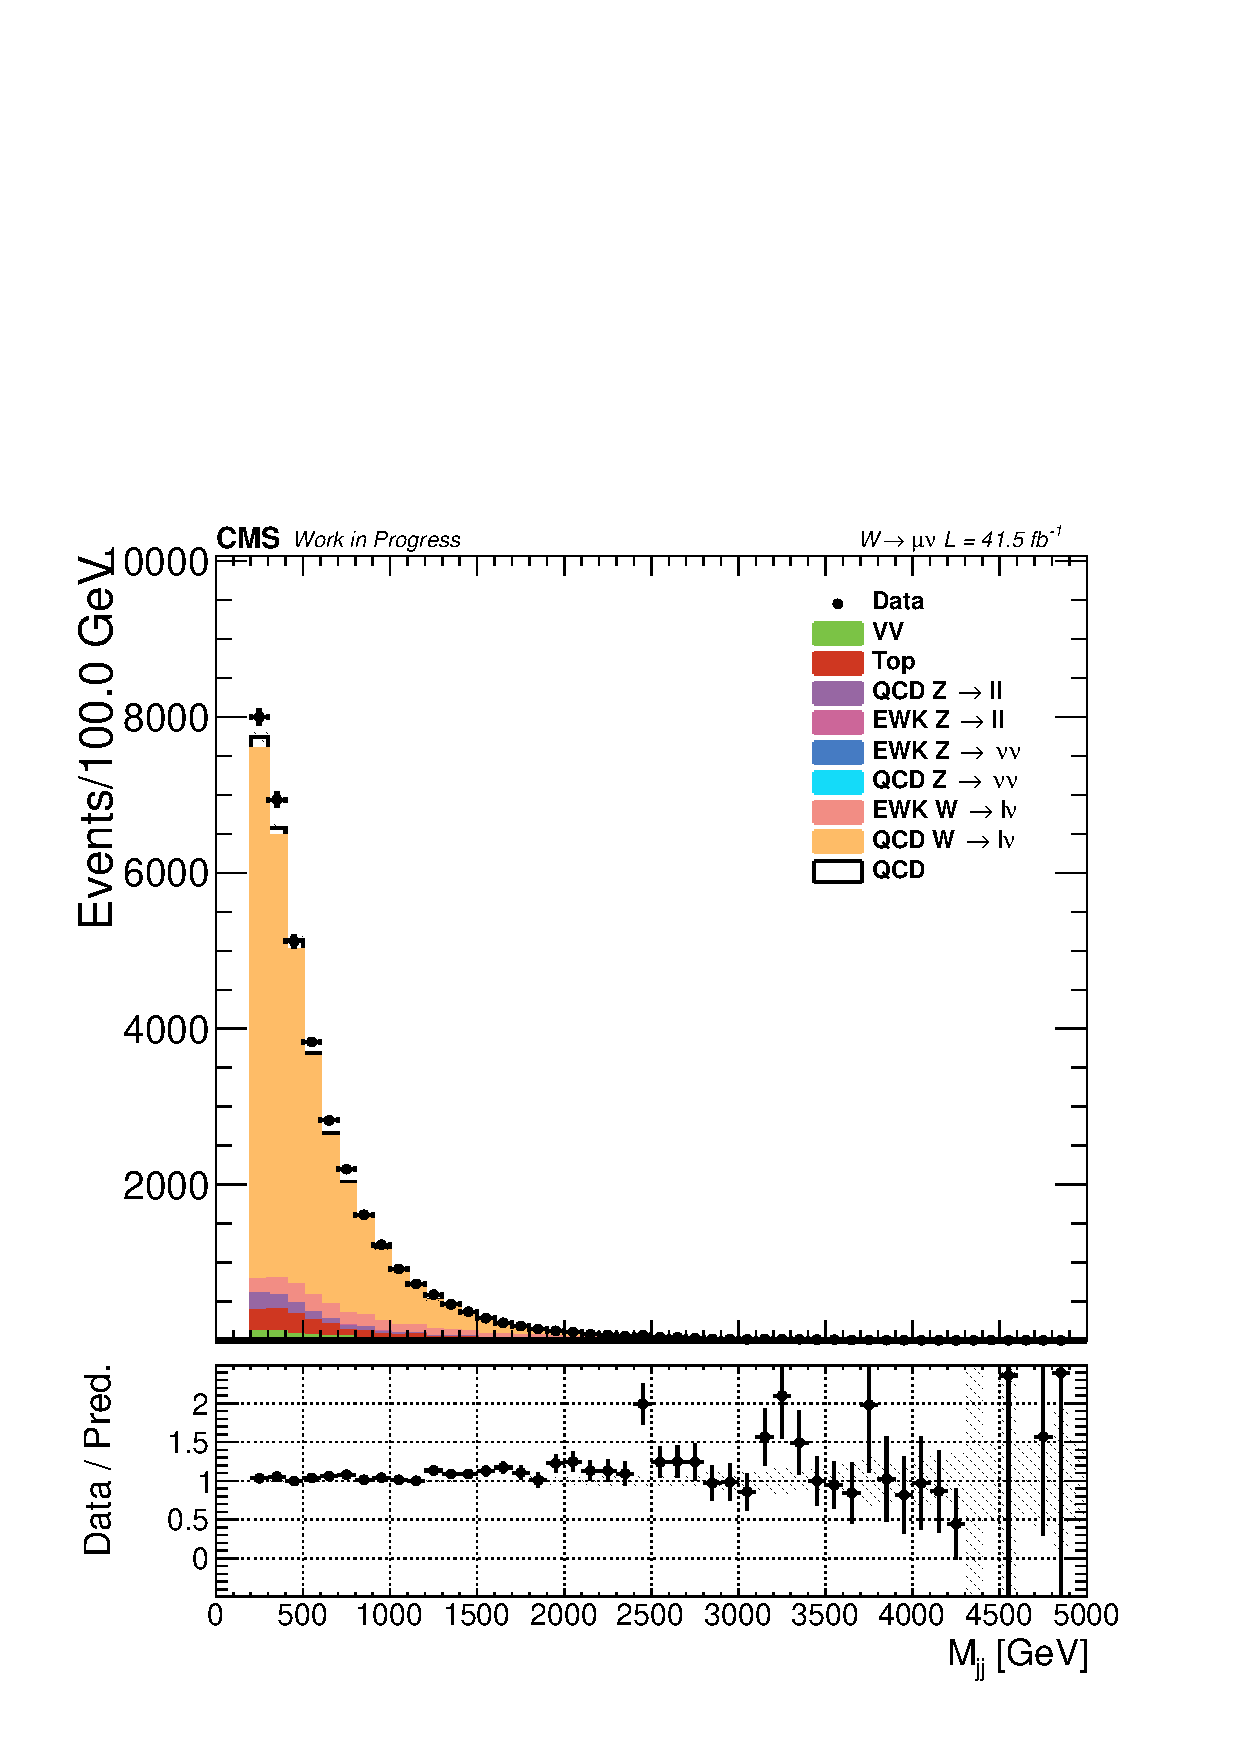
\includegraphics[width=0.49\textwidth]{Control_Regions/2017_MTR/Wmunu/leadingJet_mjj.pdf}
    }
    \subfigure[$E_{T,miss}$ - MTR]{
    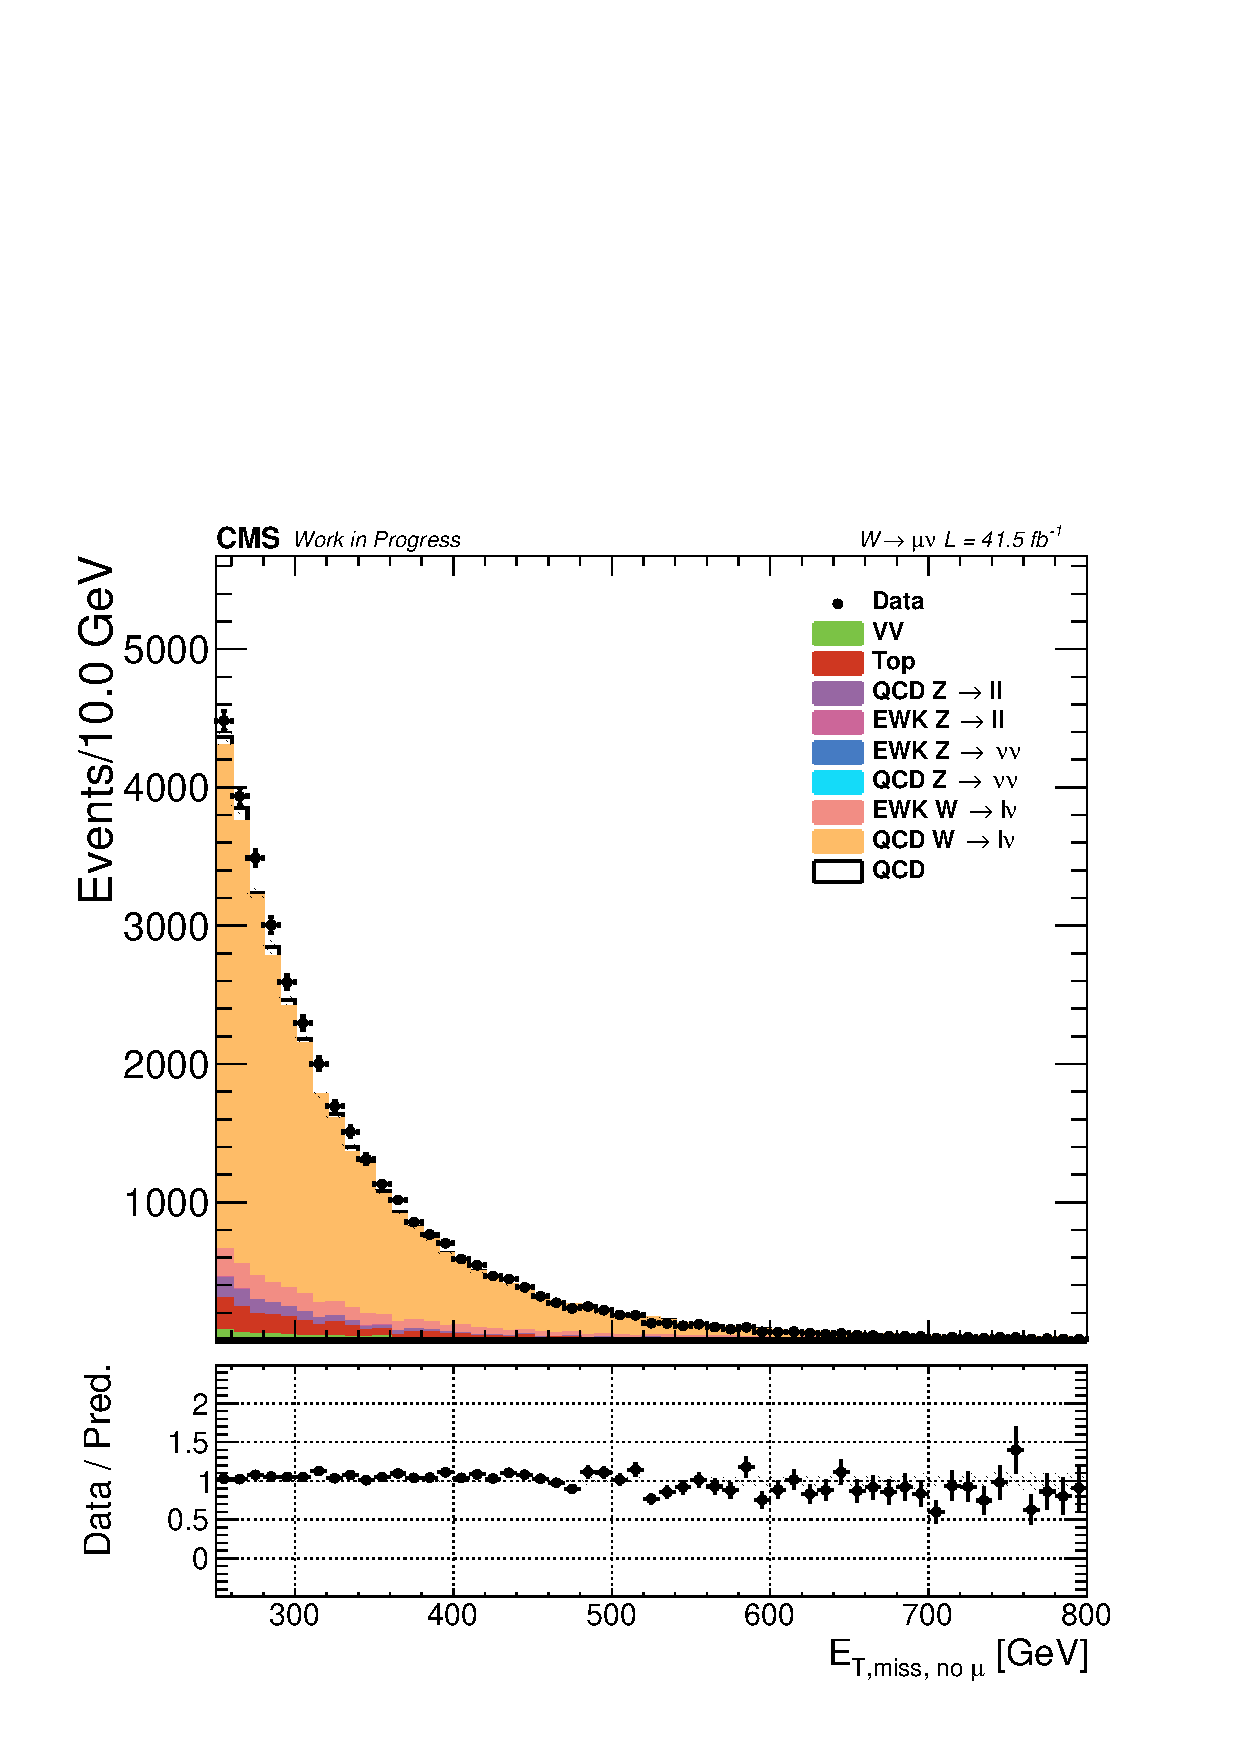
\includegraphics[width=0.49\textwidth]{Control_Regions/2017_MTR/Wmunu/MetNoMu.pdf}
    }\\
    \subfigure[$m_{jj}$ - VTR]{
    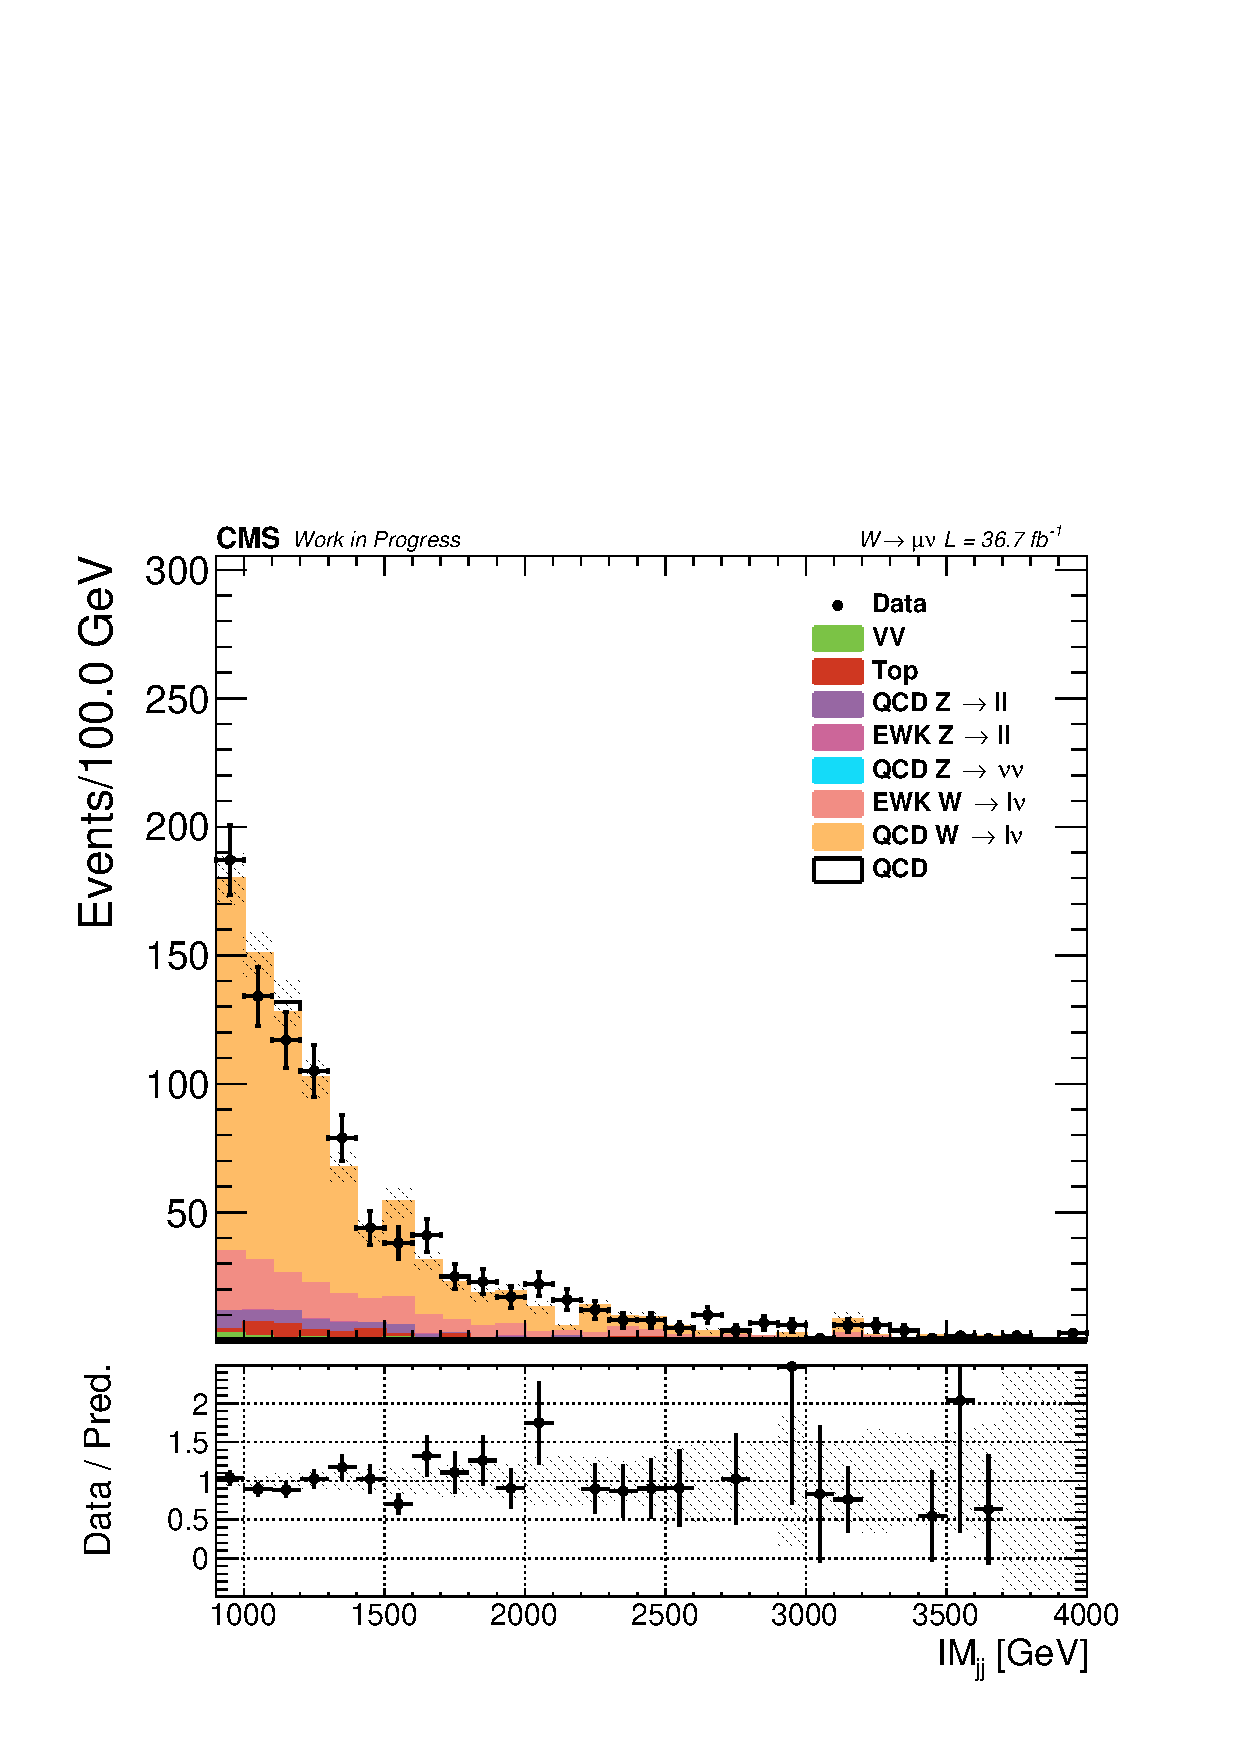
\includegraphics[width=0.49\textwidth]{Control_Regions/2017_VTR/Wmunu/lMjj.pdf}
    }
    \subfigure[$E_{T,miss}$ - VTR]{
    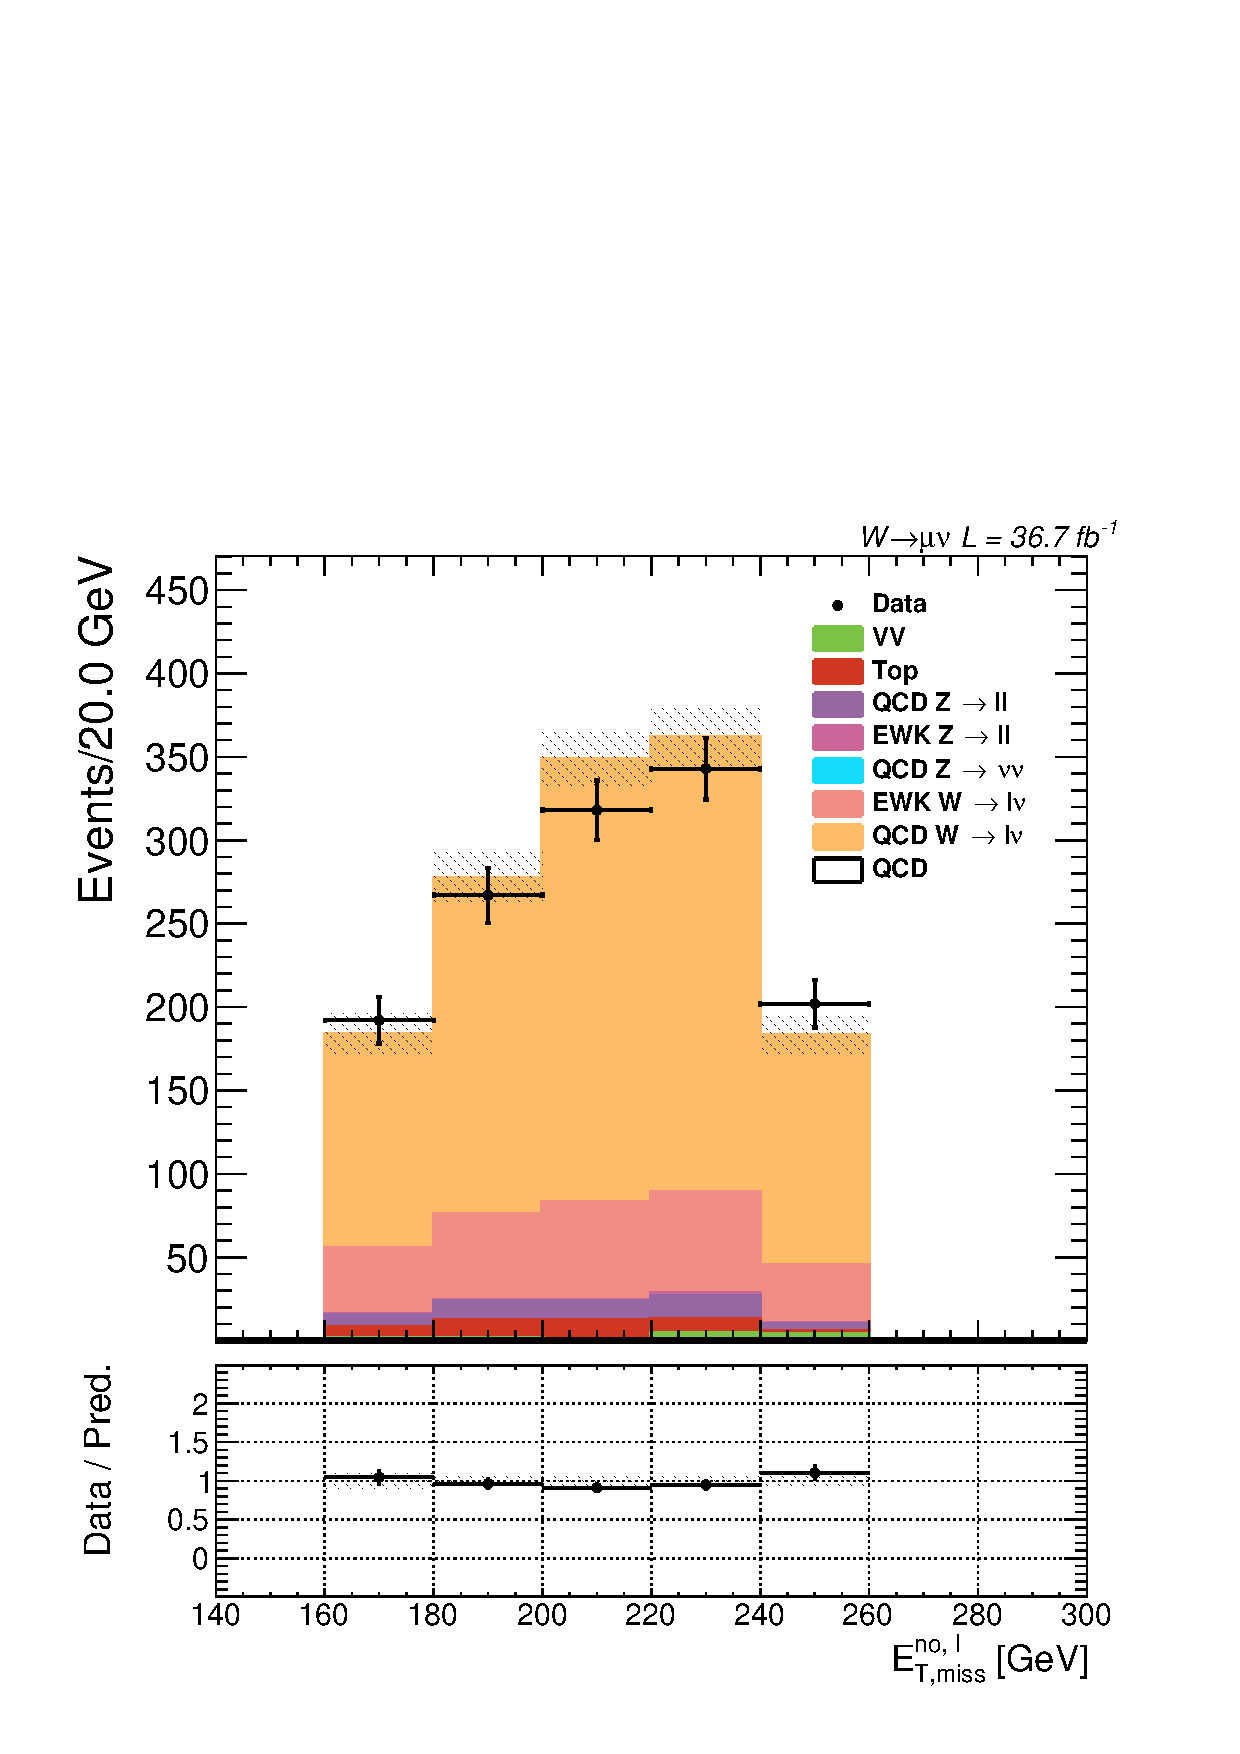
\includegraphics[width=0.49\textwidth]{Control_Regions/2017_VTR/Wmunu/MetNoMu.pdf}
    }
  \caption{Distributions of $mjj$ and $E_{T,miss}$ variables in single muon region for MTR (top) and VTR (bottom) categories for the 2017 era of data taking.}
  \label{fig:2017_Wmunu_1}
\end{figure}

\begin{figure}[htbp]
  \centering
    \subfigure[$m_{jj}$ - MTR]{
    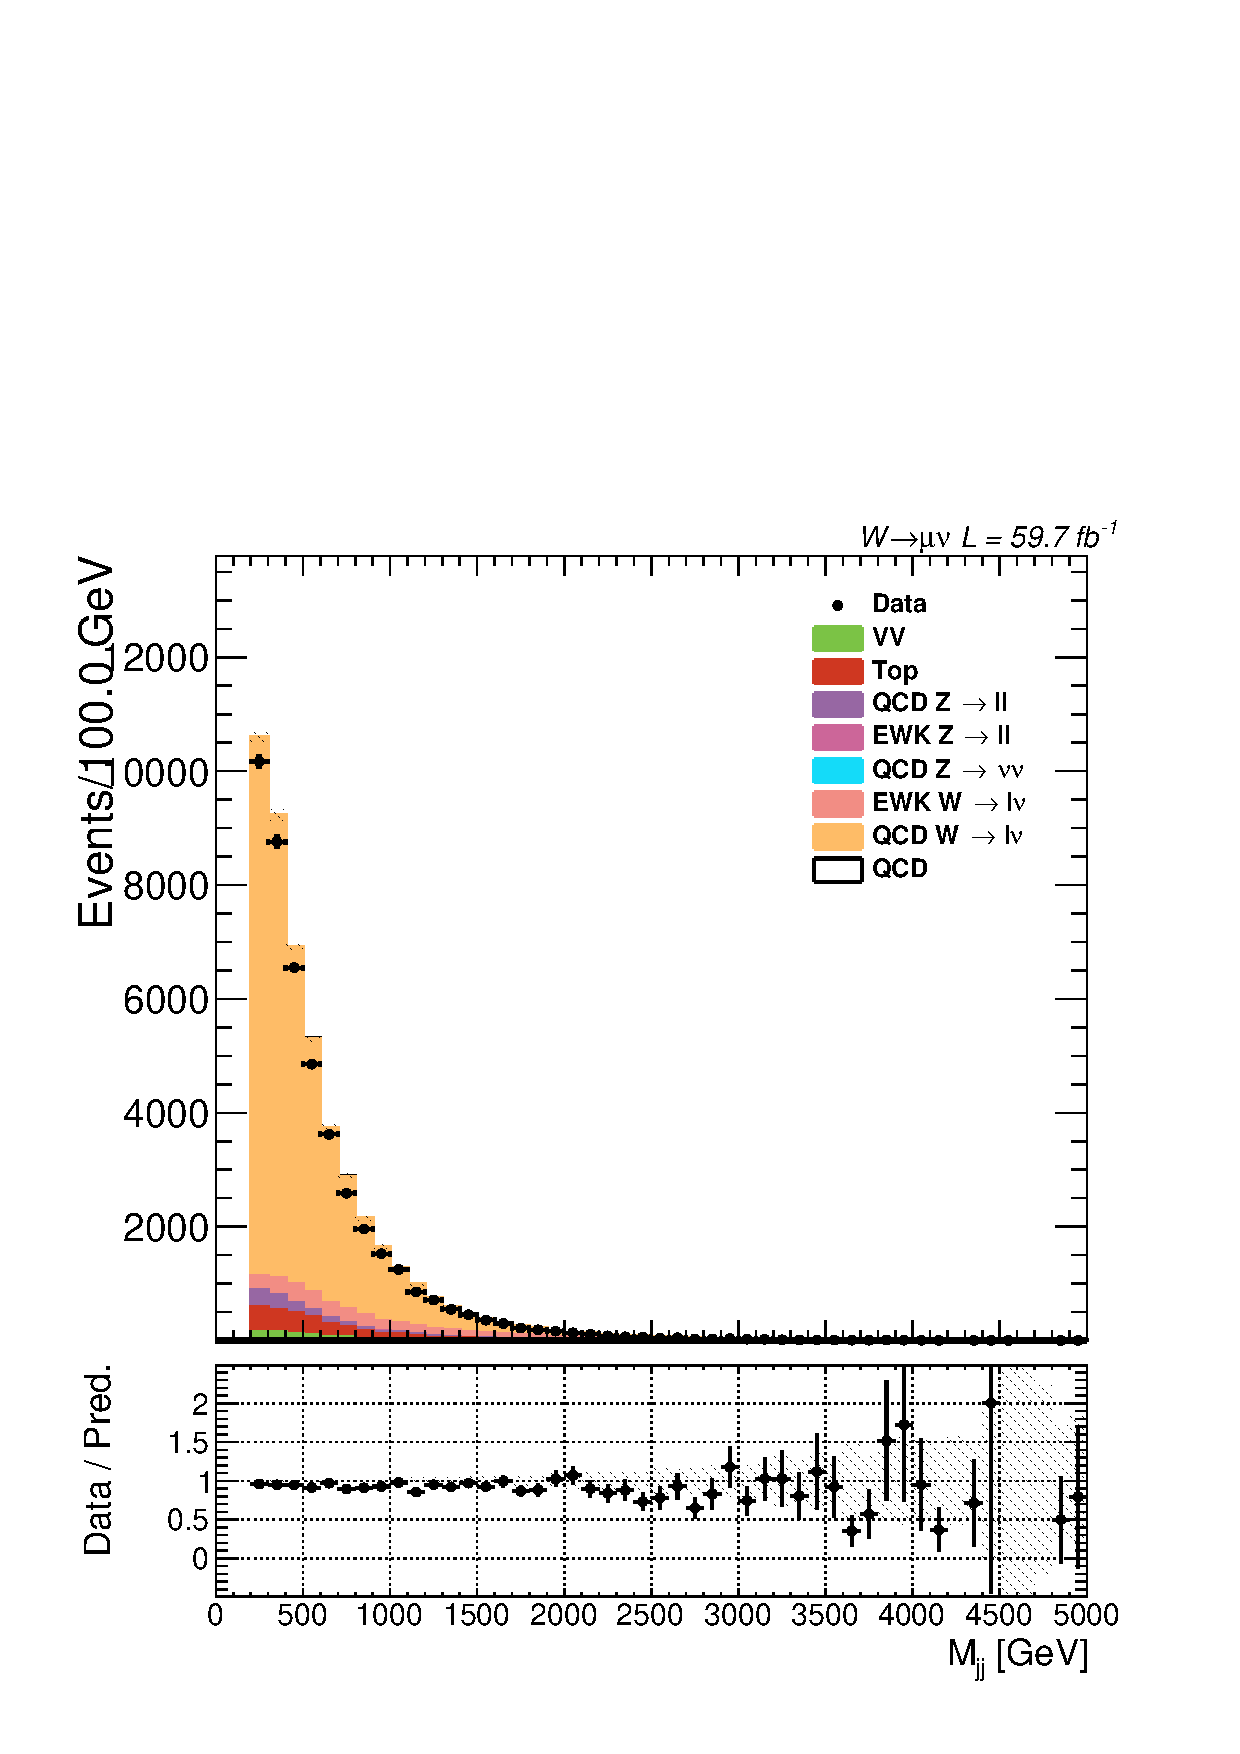
\includegraphics[width=0.49\textwidth]{Control_Regions/2018_MTR/Wmunu/leadingJet_mjj.pdf}
    }
    \subfigure[$E_{T,miss}$ - MTR]{
    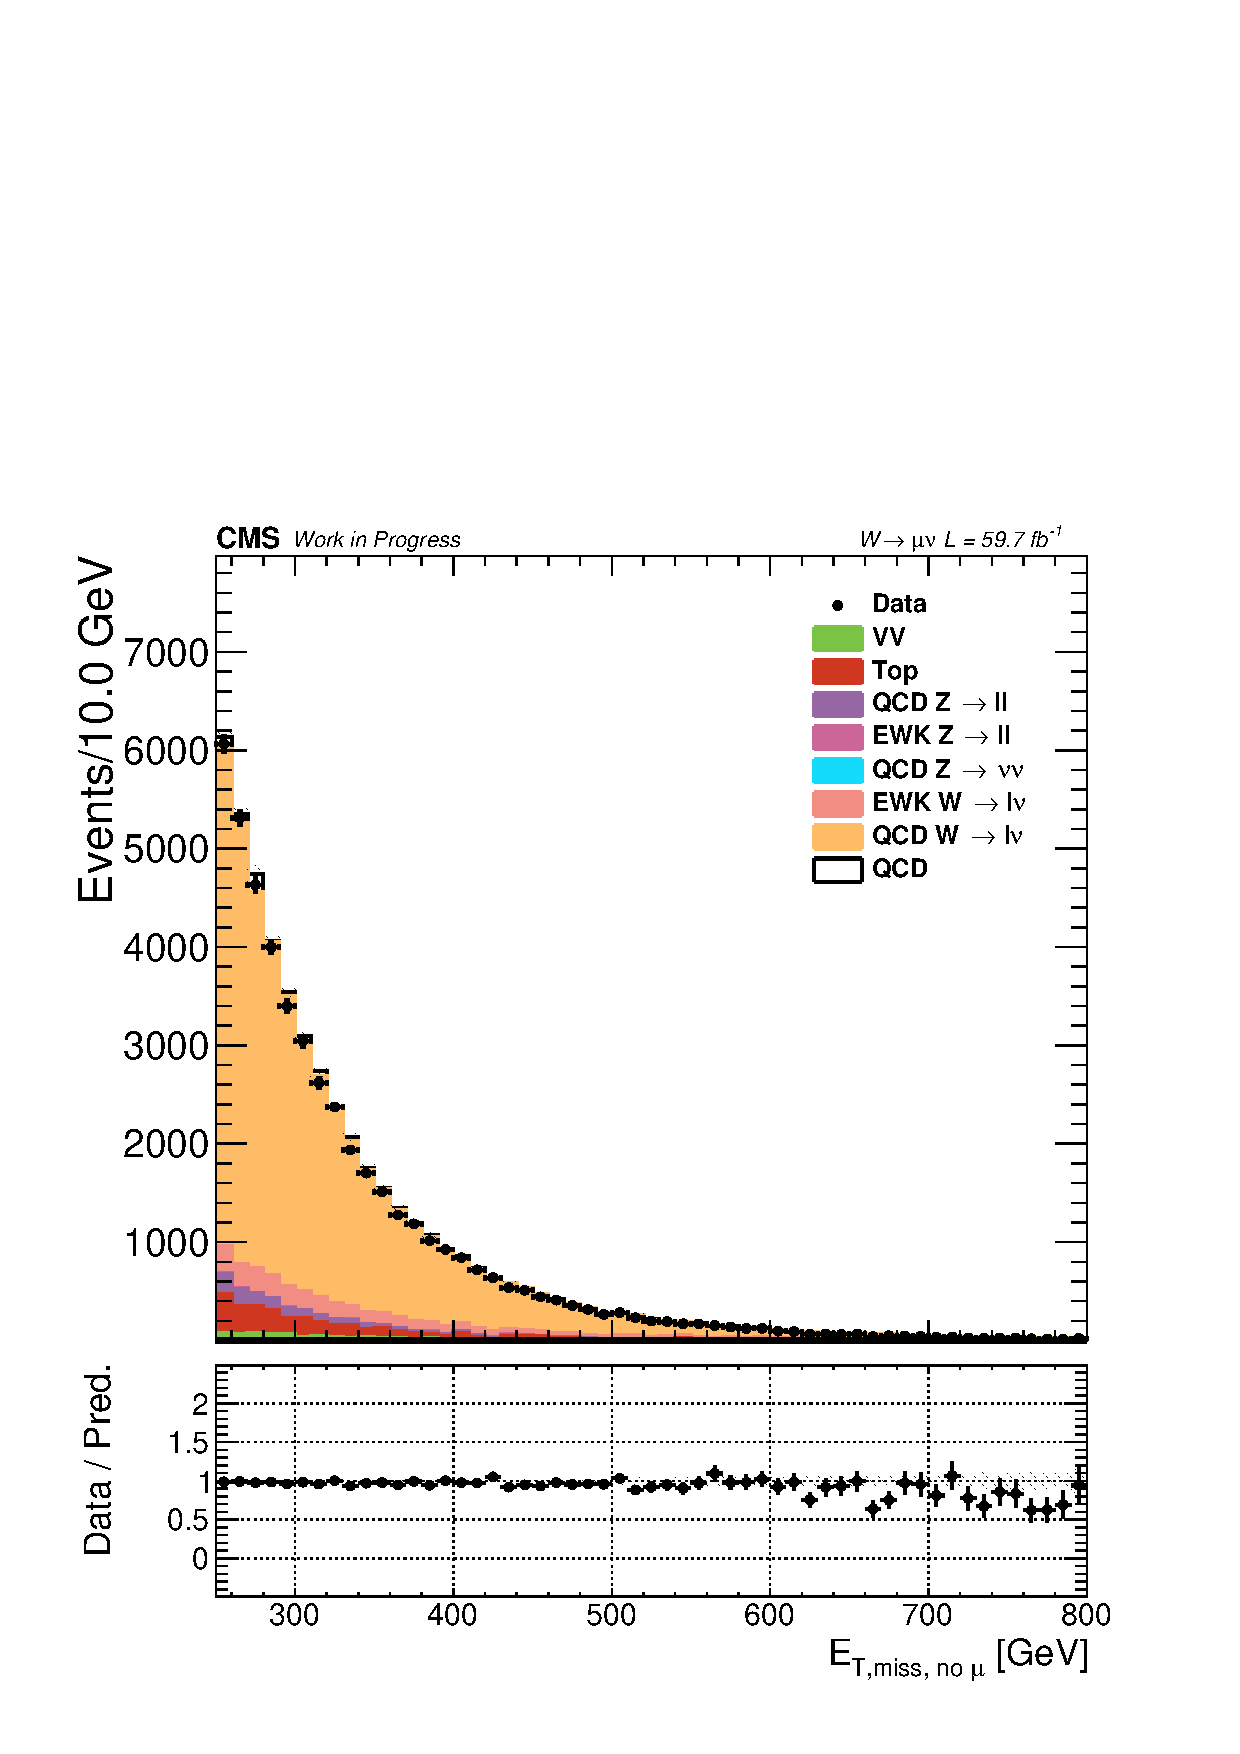
\includegraphics[width=0.49\textwidth]{Control_Regions/2018_MTR/Wmunu/MetNoMu.pdf}
    }\\
    \subfigure[$m_{jj}$ - VTR]{
    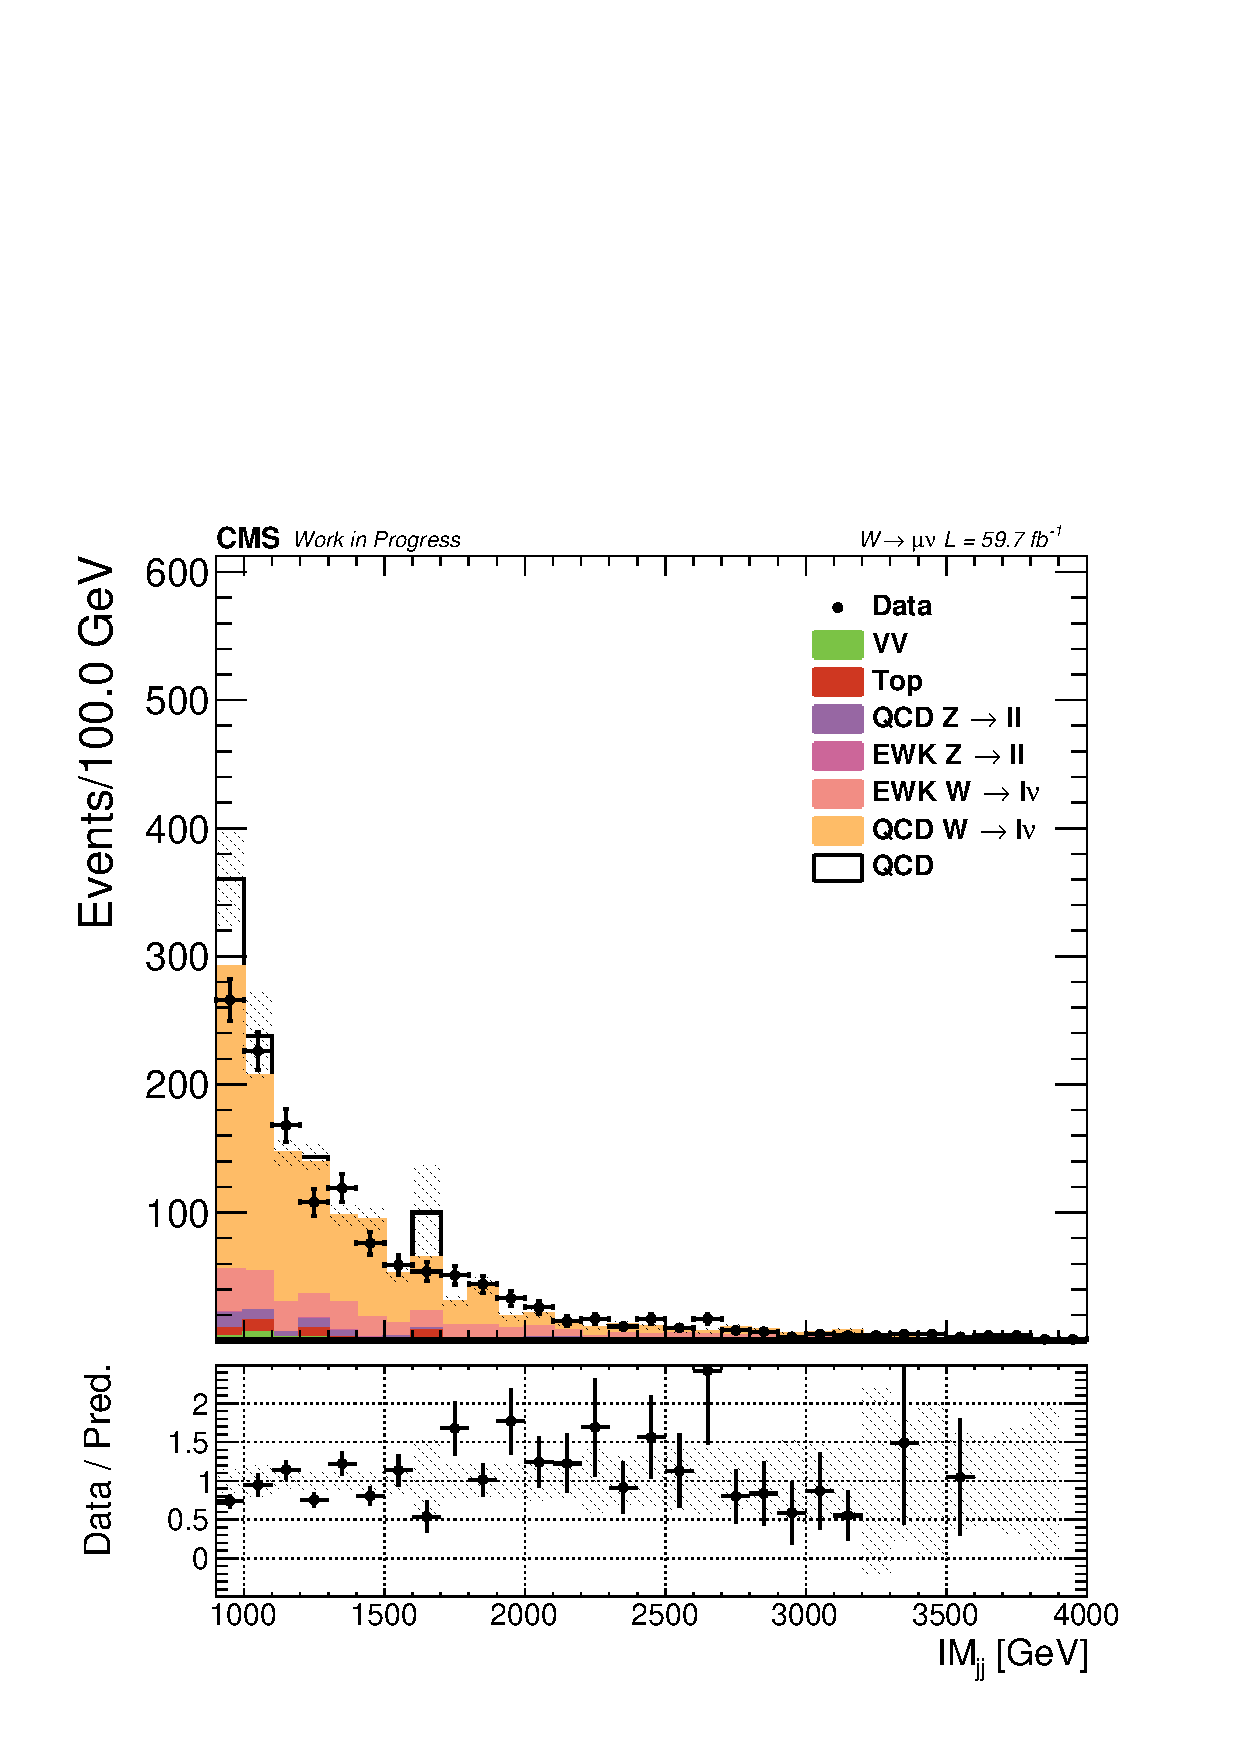
\includegraphics[width=0.49\textwidth]{Control_Regions/2018_VTR/Wmunu/lMjj.pdf}
    }
    \subfigure[$E_{T,miss}$ - VTR]{
    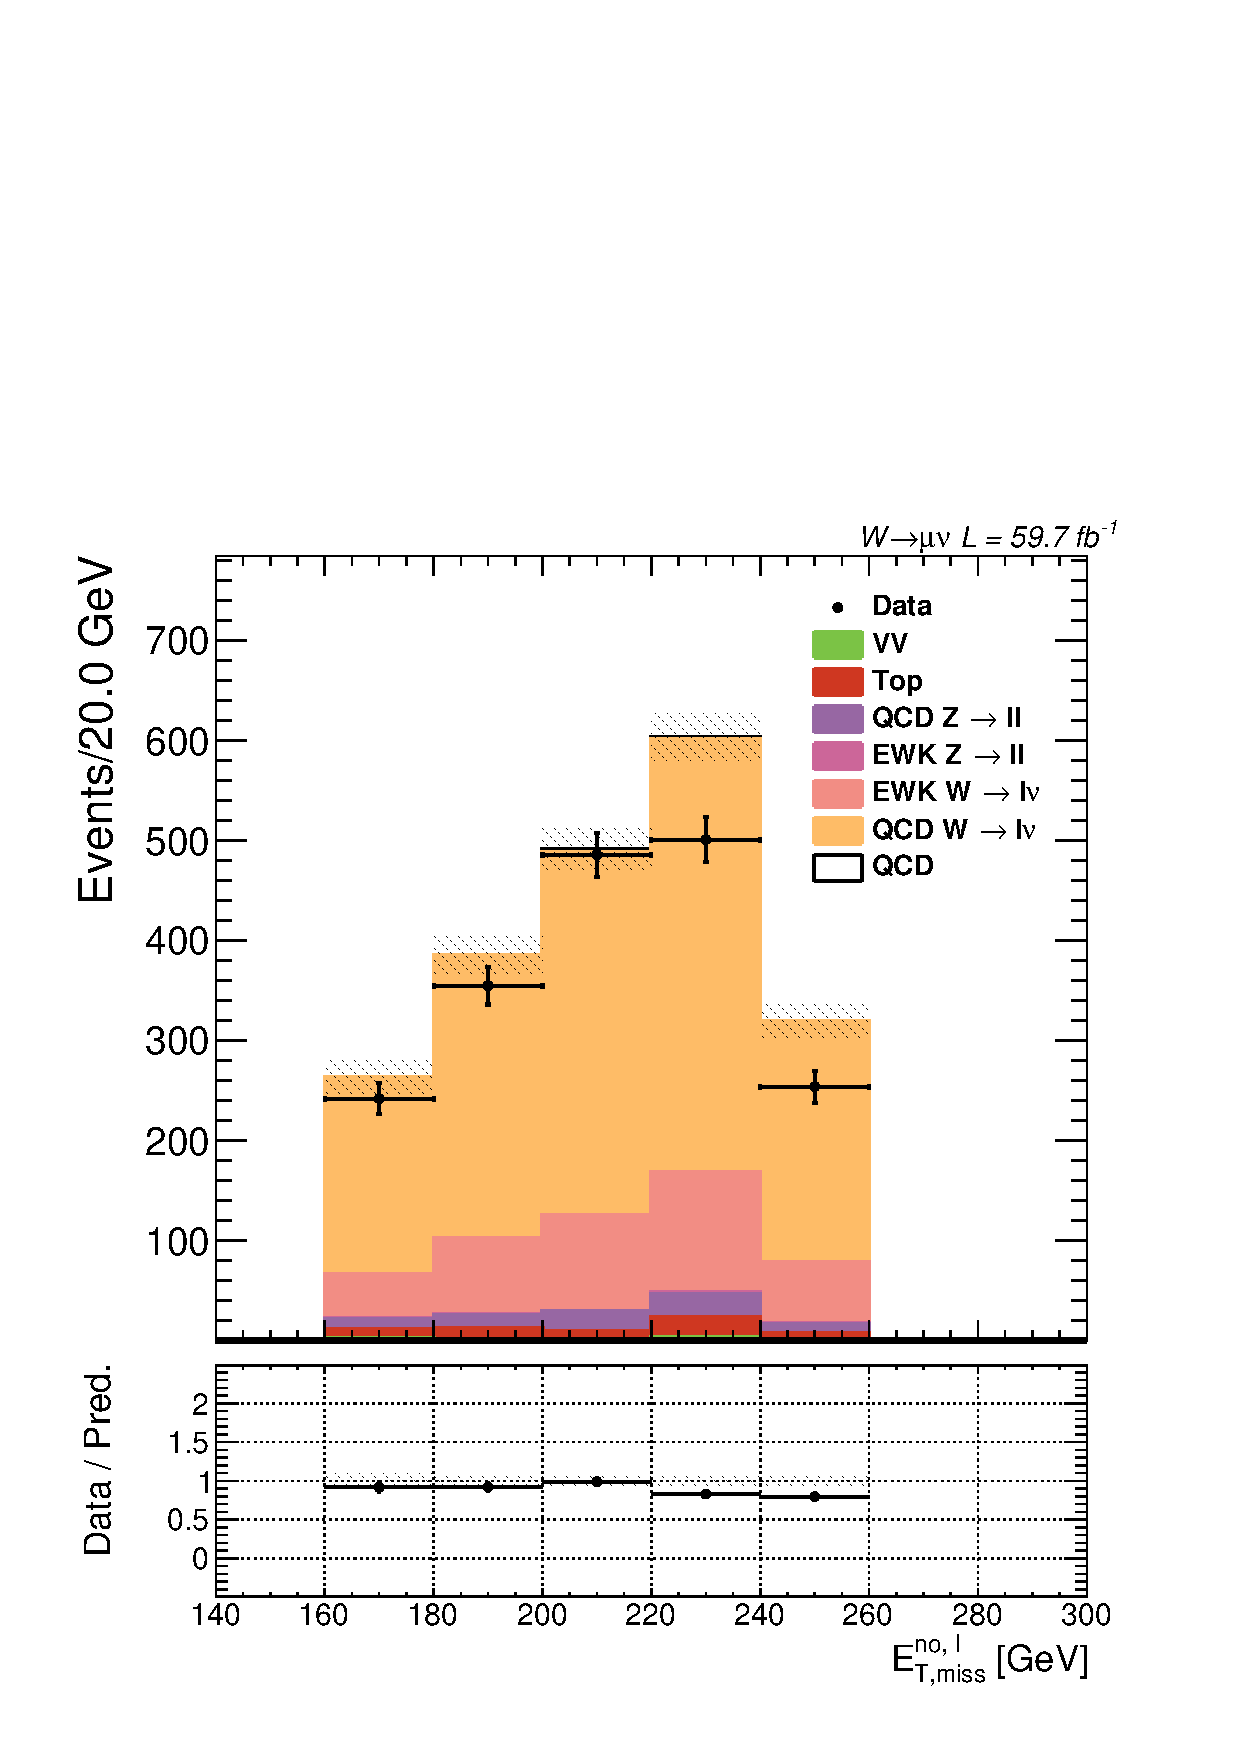
\includegraphics[width=0.49\textwidth]{Control_Regions/2018_VTR/Wmunu/MetNoMu.pdf}
    }
  \caption{Distributions of $mjj$ and $E_{T,miss}$ variables in single muon region for MTR (top) and VTR (bottom) categories for the 2018 era of data taking.}
  \label{fig:2018_Wmunu_1}
\end{figure}


\begin{figure}[htbp]
  \centering
    \subfigure[$M_{T,\mu}$ - MTR]{
    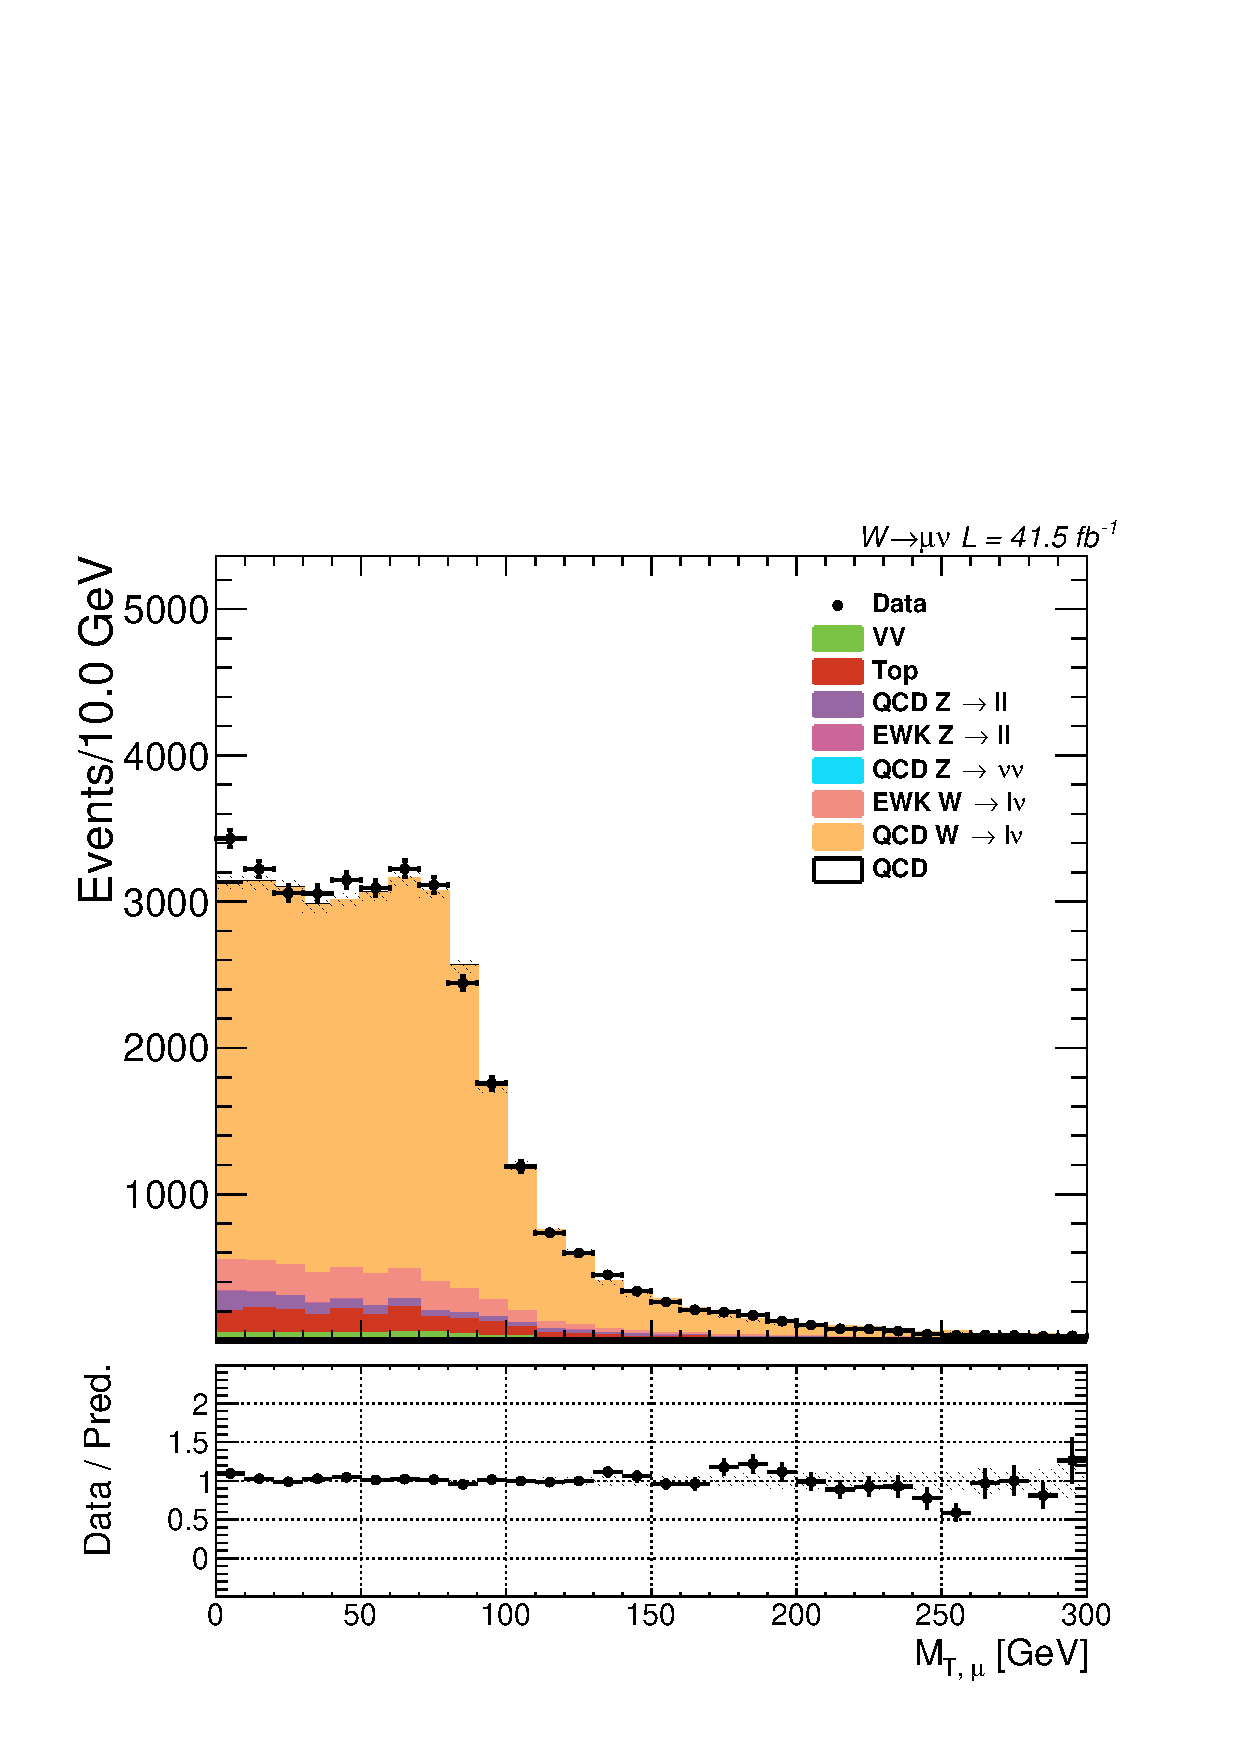
\includegraphics[width=0.49\textwidth]{Control_Regions/2017_MTR/Wmunu/MTmu_FAST.pdf}
    }
    \subfigure[\mindphinomu - MTR]{
    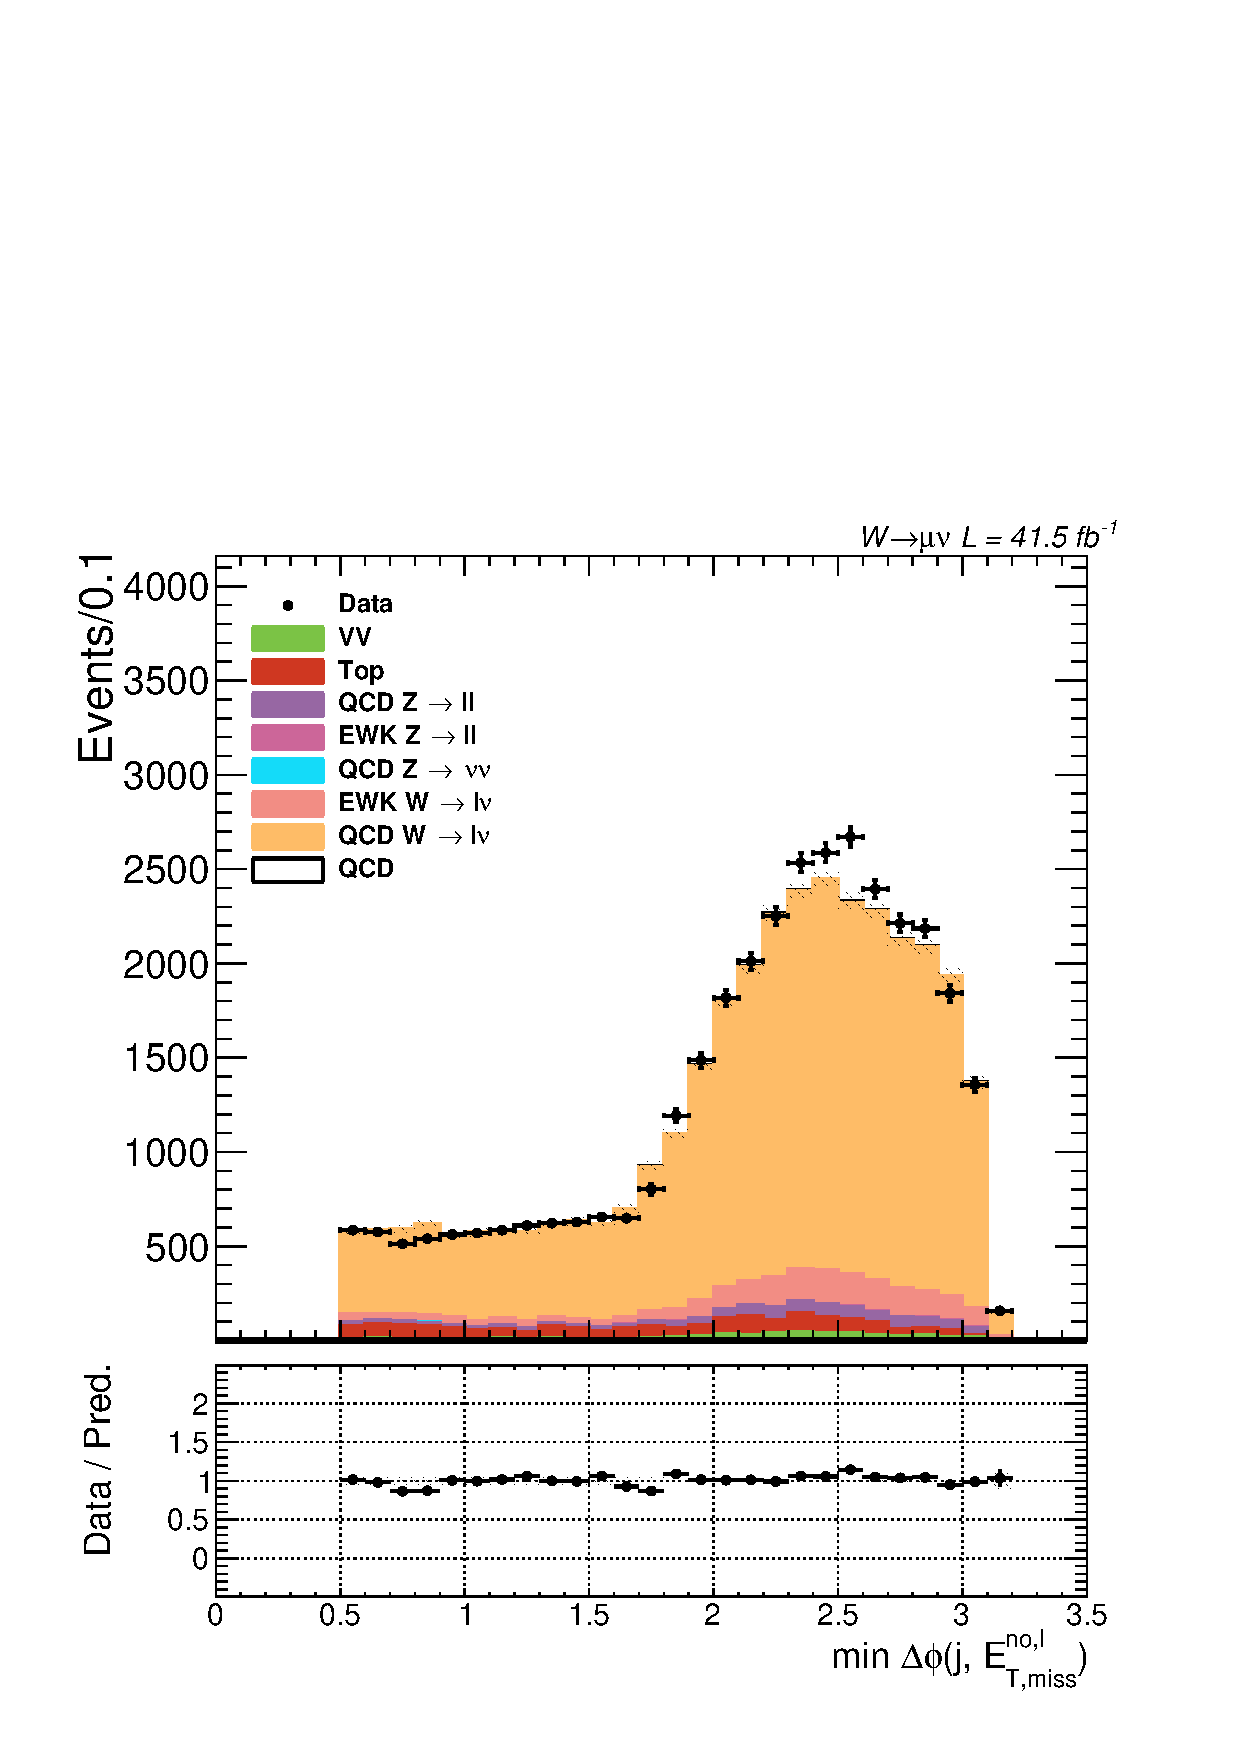
\includegraphics[width=0.49\textwidth]{Control_Regions/2017_MTR/Wmunu/MetNoLep_CleanJet_mindPhi.pdf}
    }\\
    \subfigure[$M_{T,\mu}$ - VTR]{
    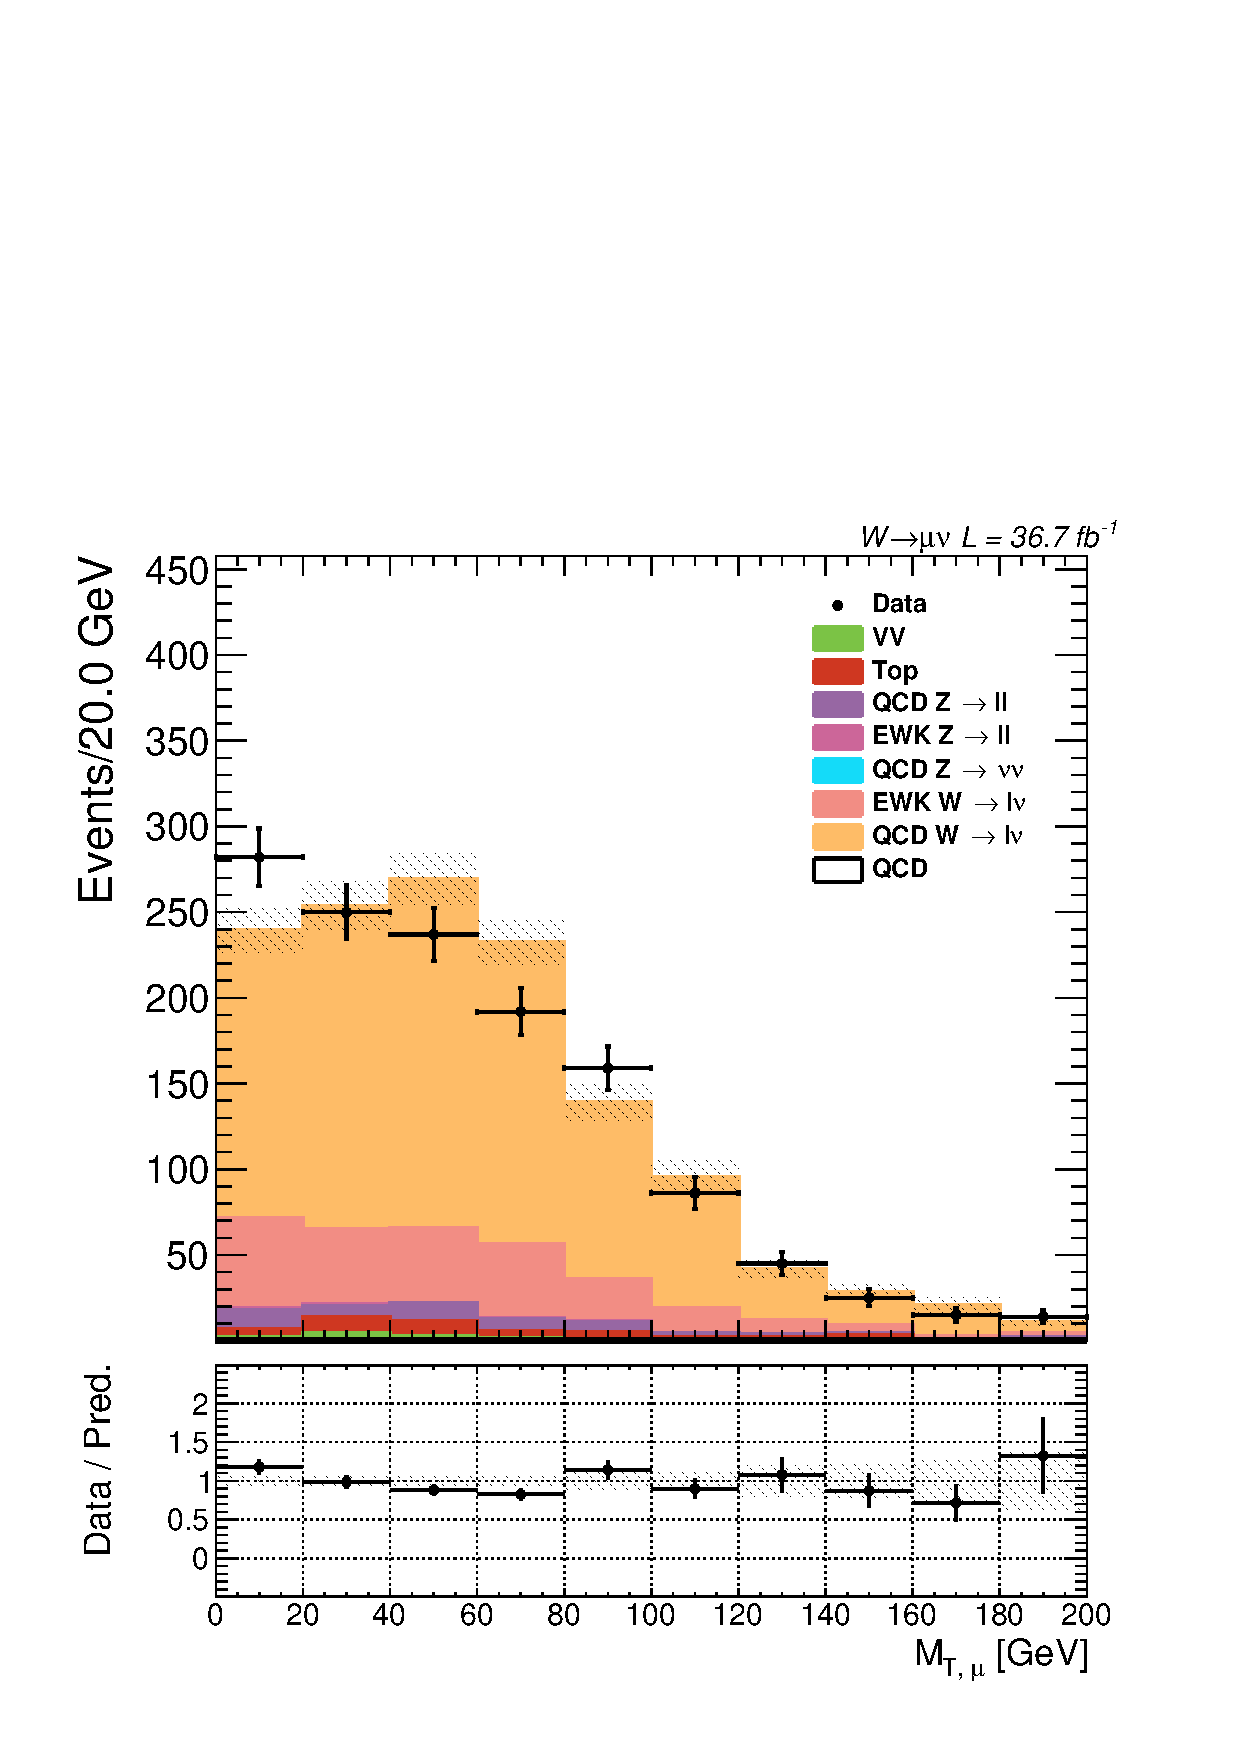
\includegraphics[width=0.49\textwidth]{Control_Regions/2017_VTR/Wmunu/MTmu_FAST.pdf}
    }
    \subfigure[\mindphinomu - VTR]{
    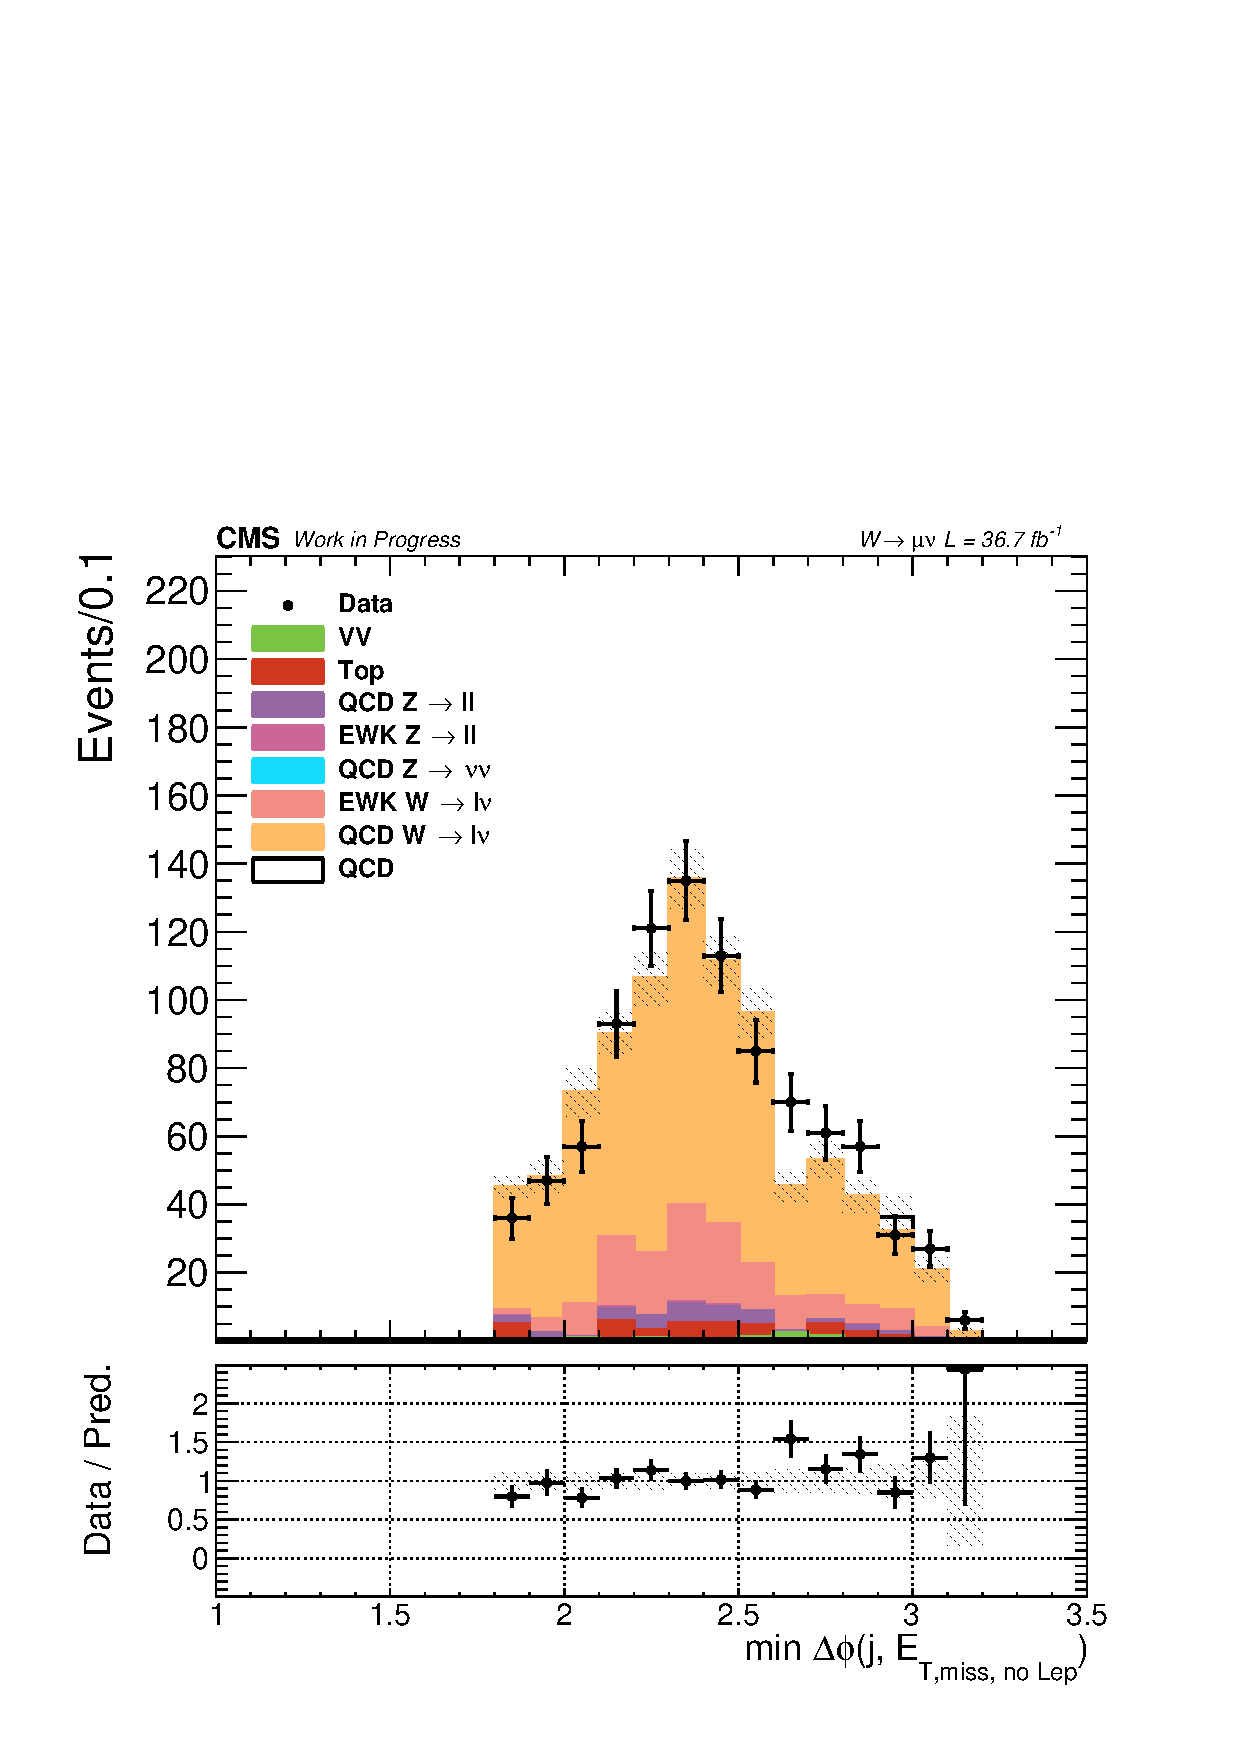
\includegraphics[width=0.49\textwidth]{Control_Regions/2017_VTR/Wmunu/MetNoLep_CleanJet_mindPhi.pdf}
    }
  \caption{Distributions of $M_{T,\mu}$ and \mindphinomu variables in single muon region for MTR (top) and VTR (bottom) categories for the 2017 era of data taking.}
  \label{fig:2017_Wmunu_2}
\end{figure}

\begin{figure}[htbp]
  \centering
    \subfigure[$M_{T,\mu}$ - MTR]{
    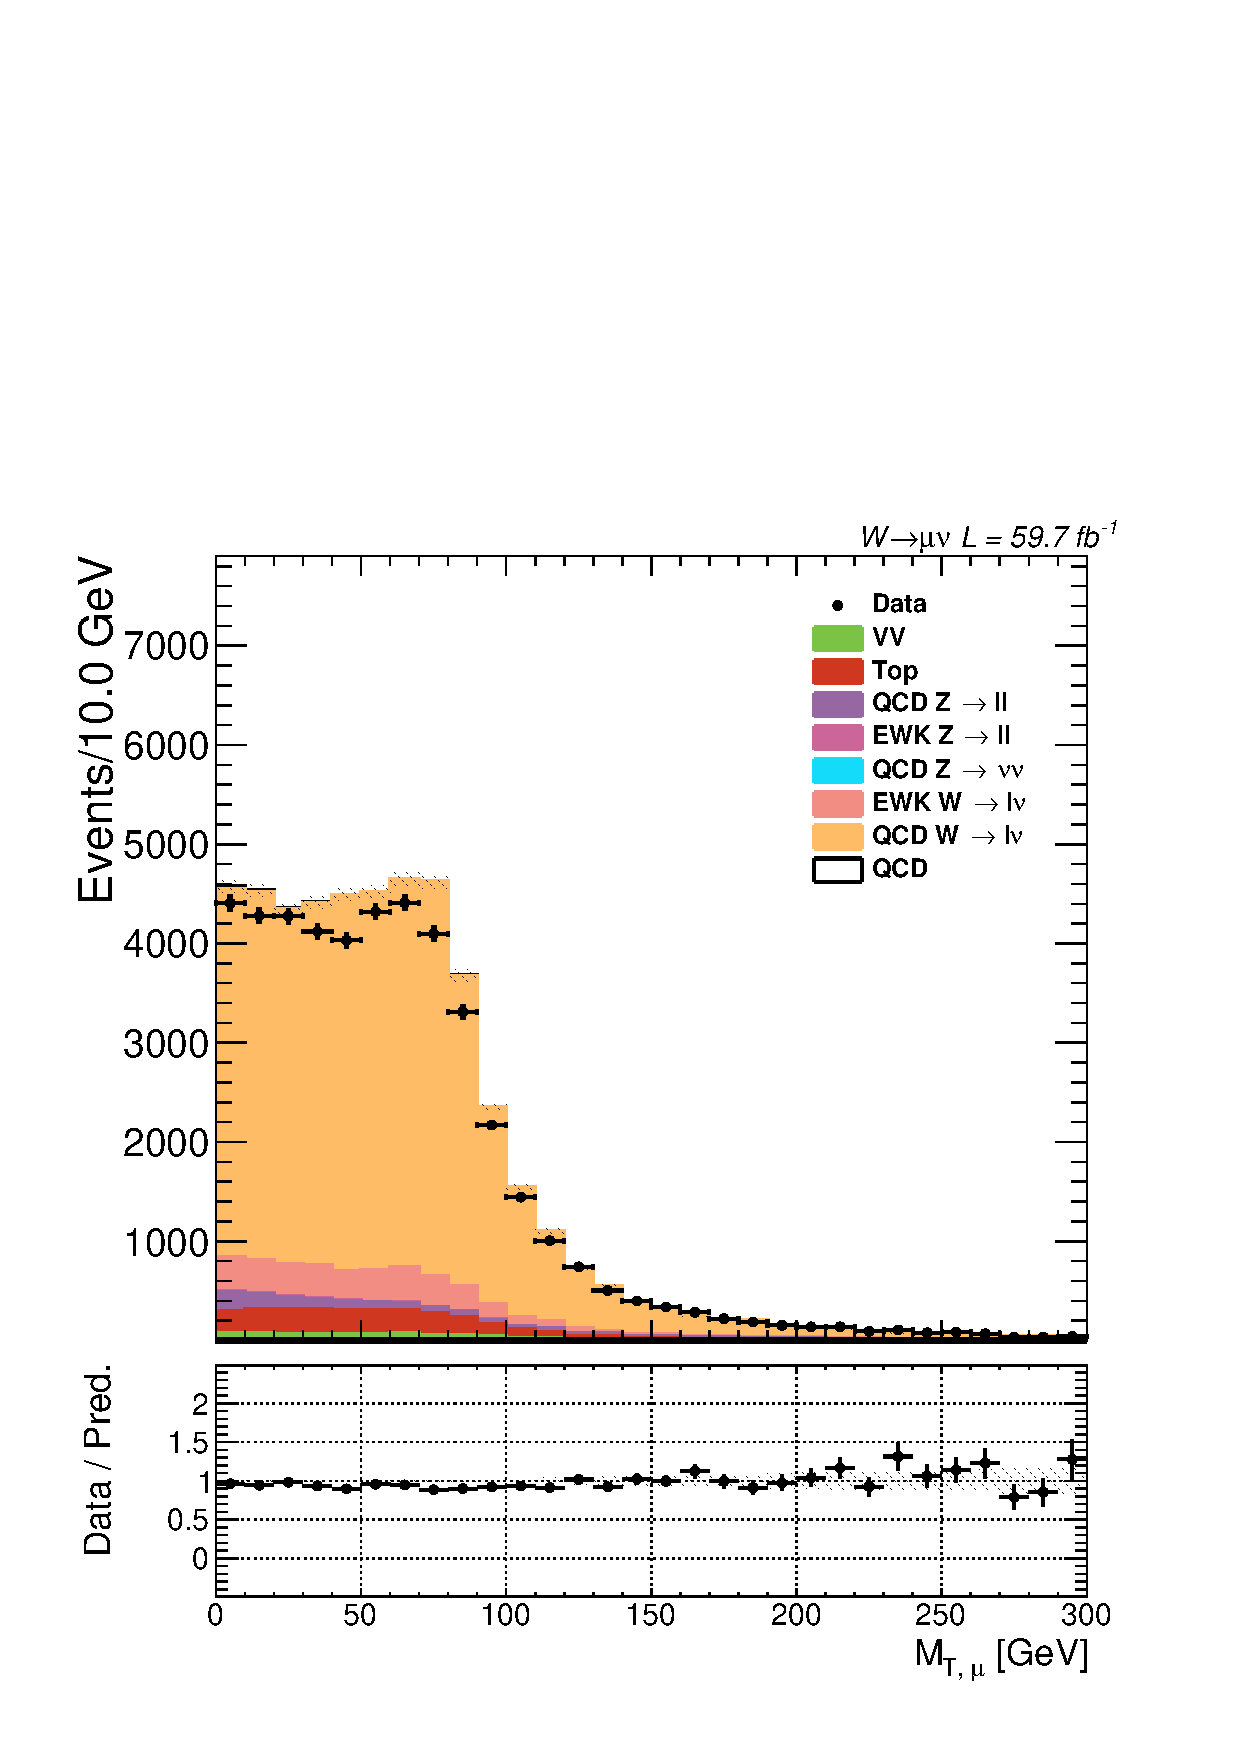
\includegraphics[width=0.49\textwidth]{Control_Regions/2018_MTR/Wmunu/MTmu_FAST.pdf}
    }
    \subfigure[\mindphinomu - MTR]{
    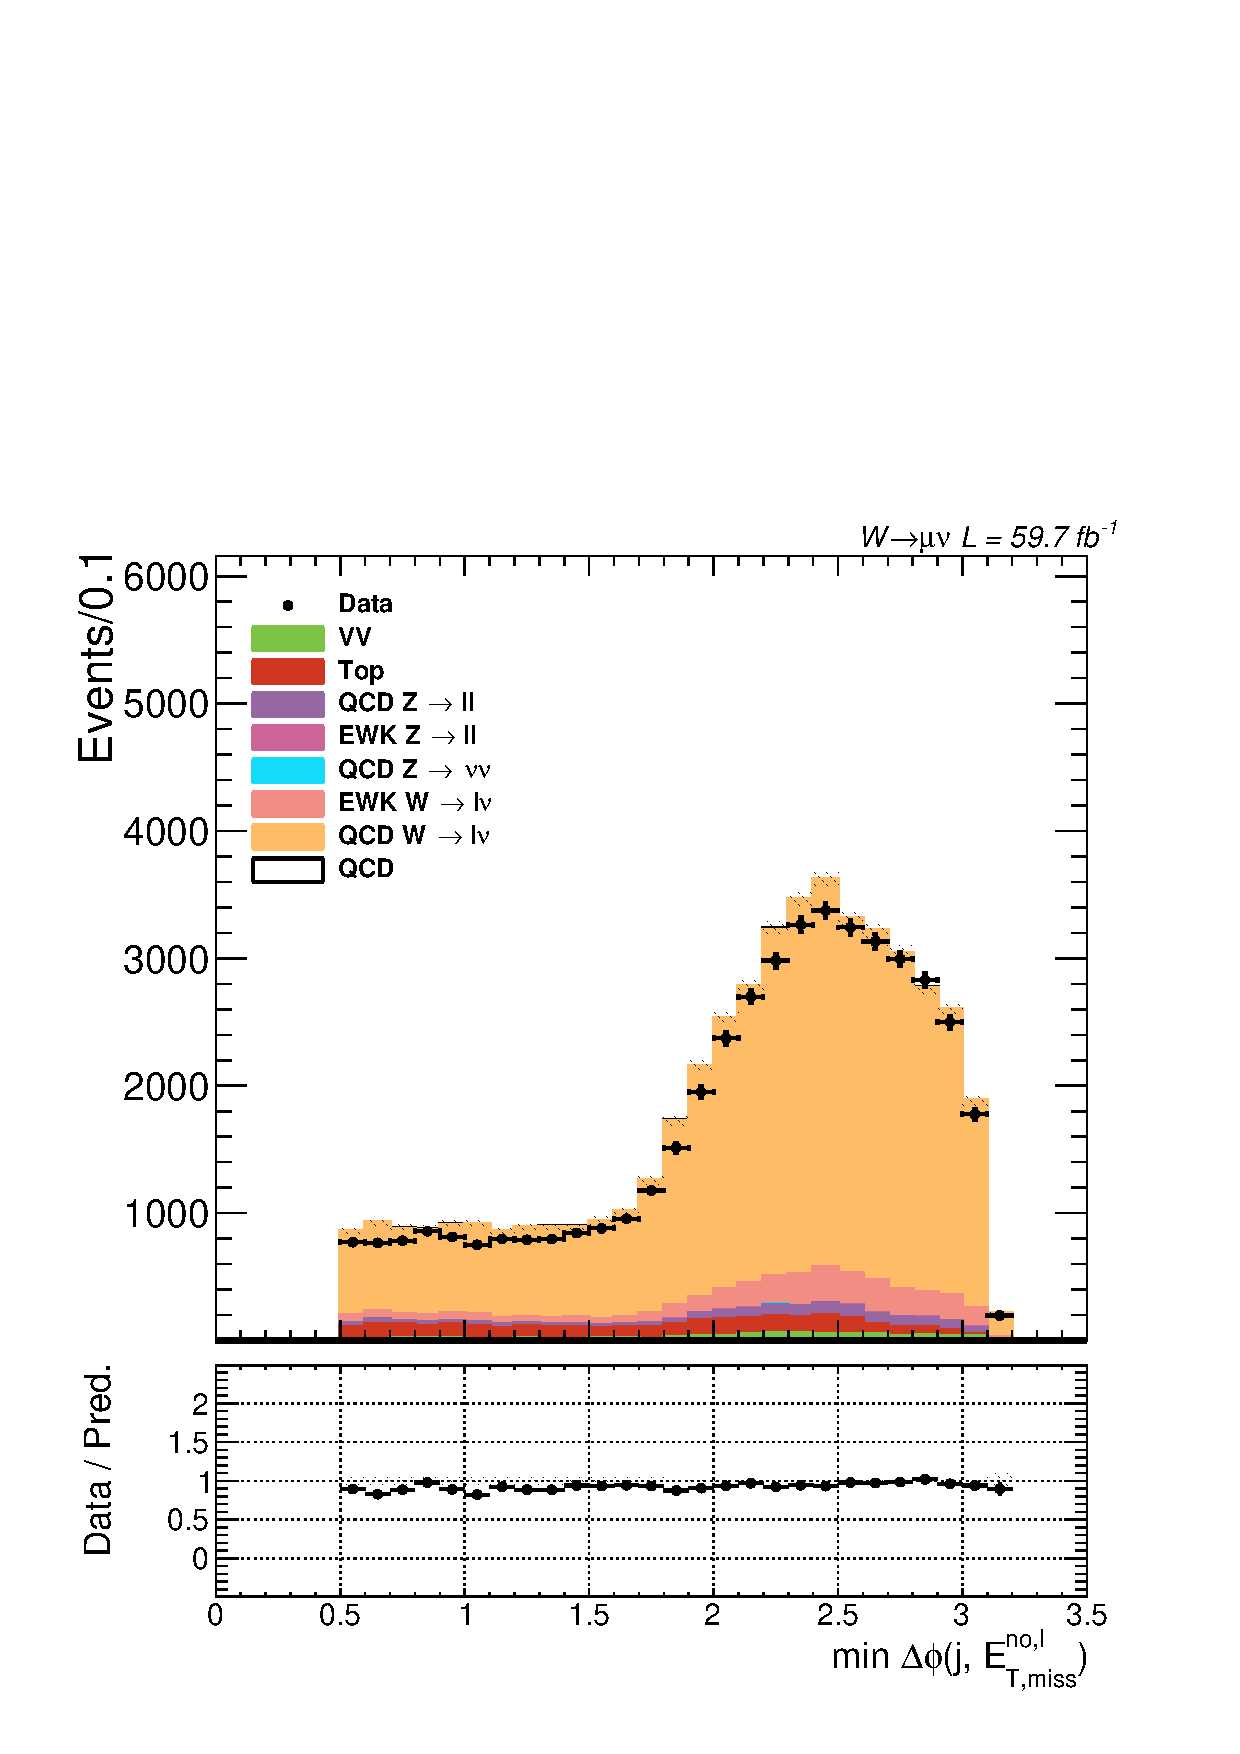
\includegraphics[width=0.49\textwidth]{Control_Regions/2018_MTR/Wmunu/MetNoLep_CleanJet_mindPhi.pdf}
    }\\
    \subfigure[$M_{T,\mu}$ - VTR]{
    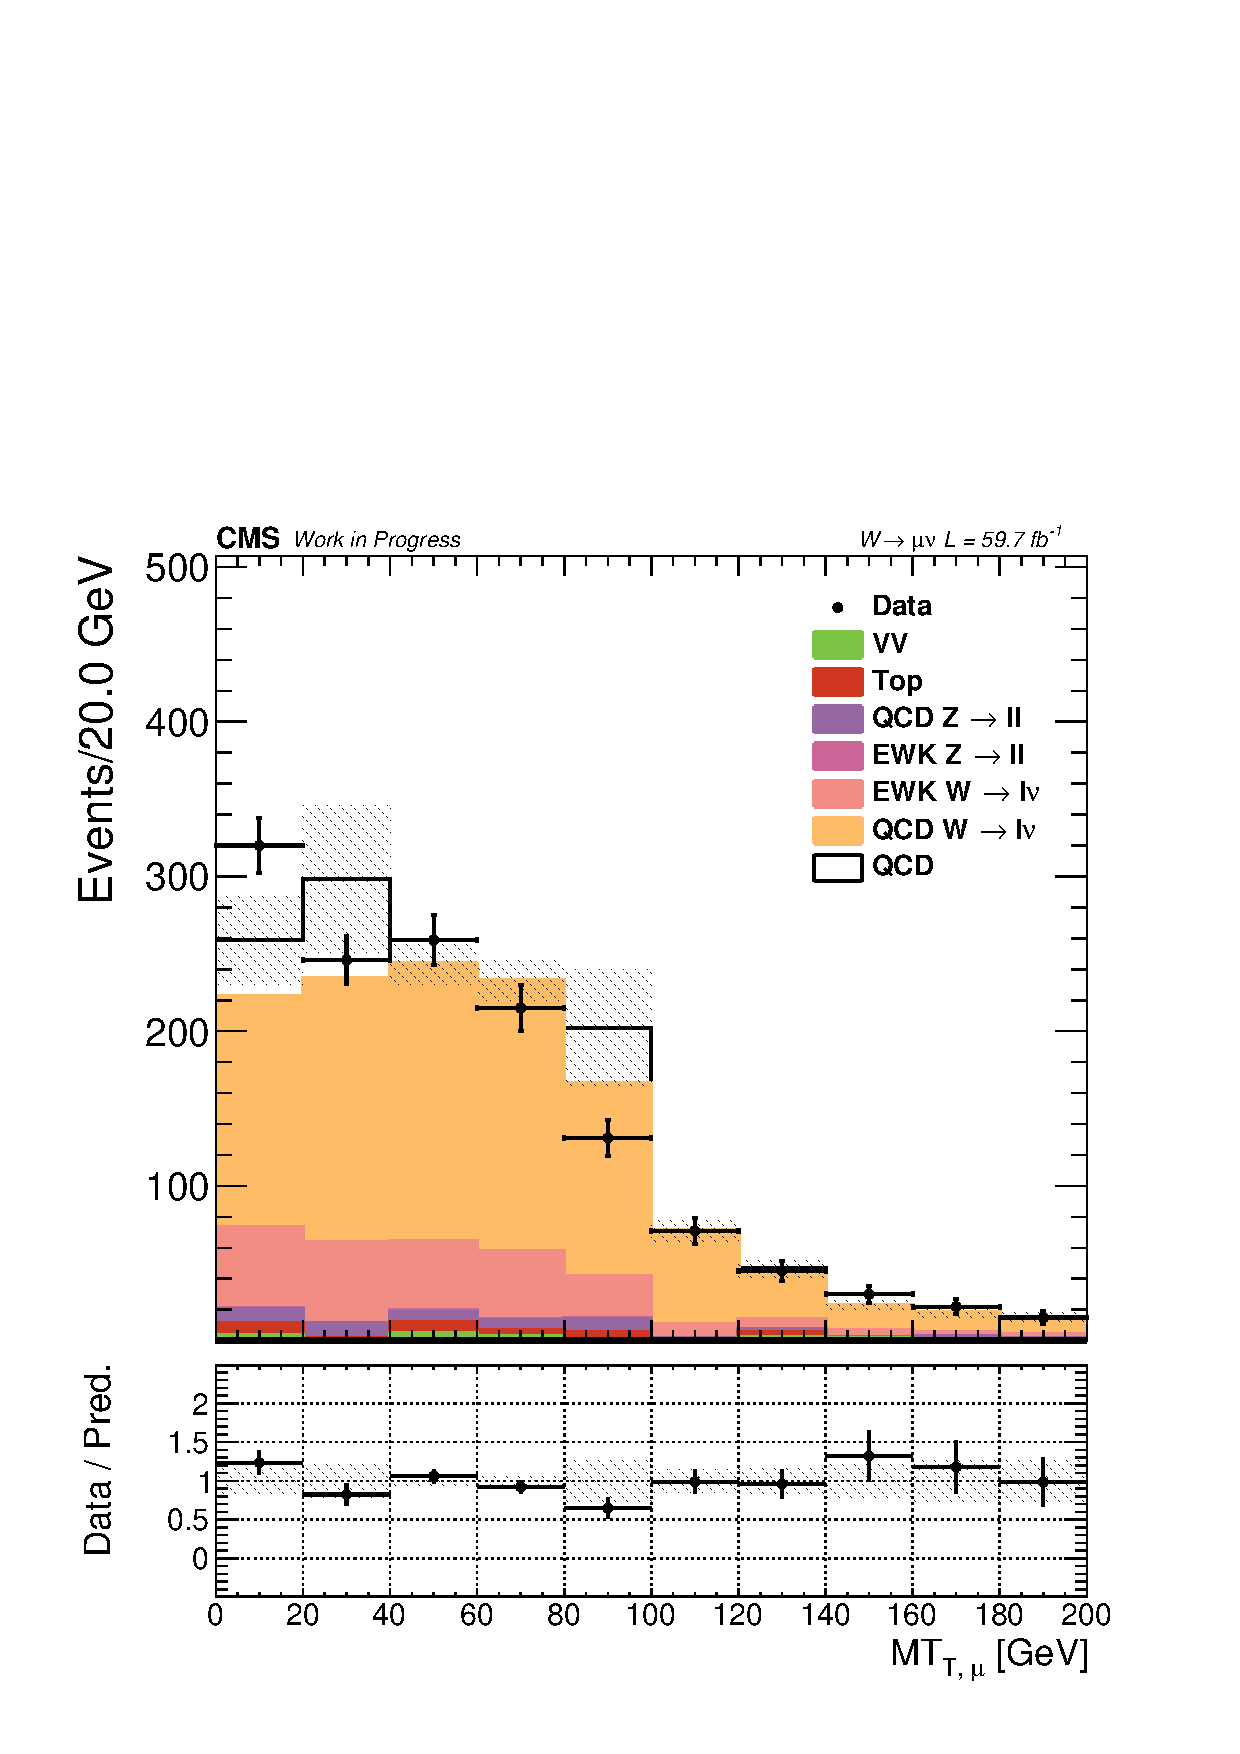
\includegraphics[width=0.49\textwidth]{Control_Regions/2018_VTR/Wmunu/MTmu_FAST.pdf}
    }
    \subfigure[\mindphinomu - VTR]{
    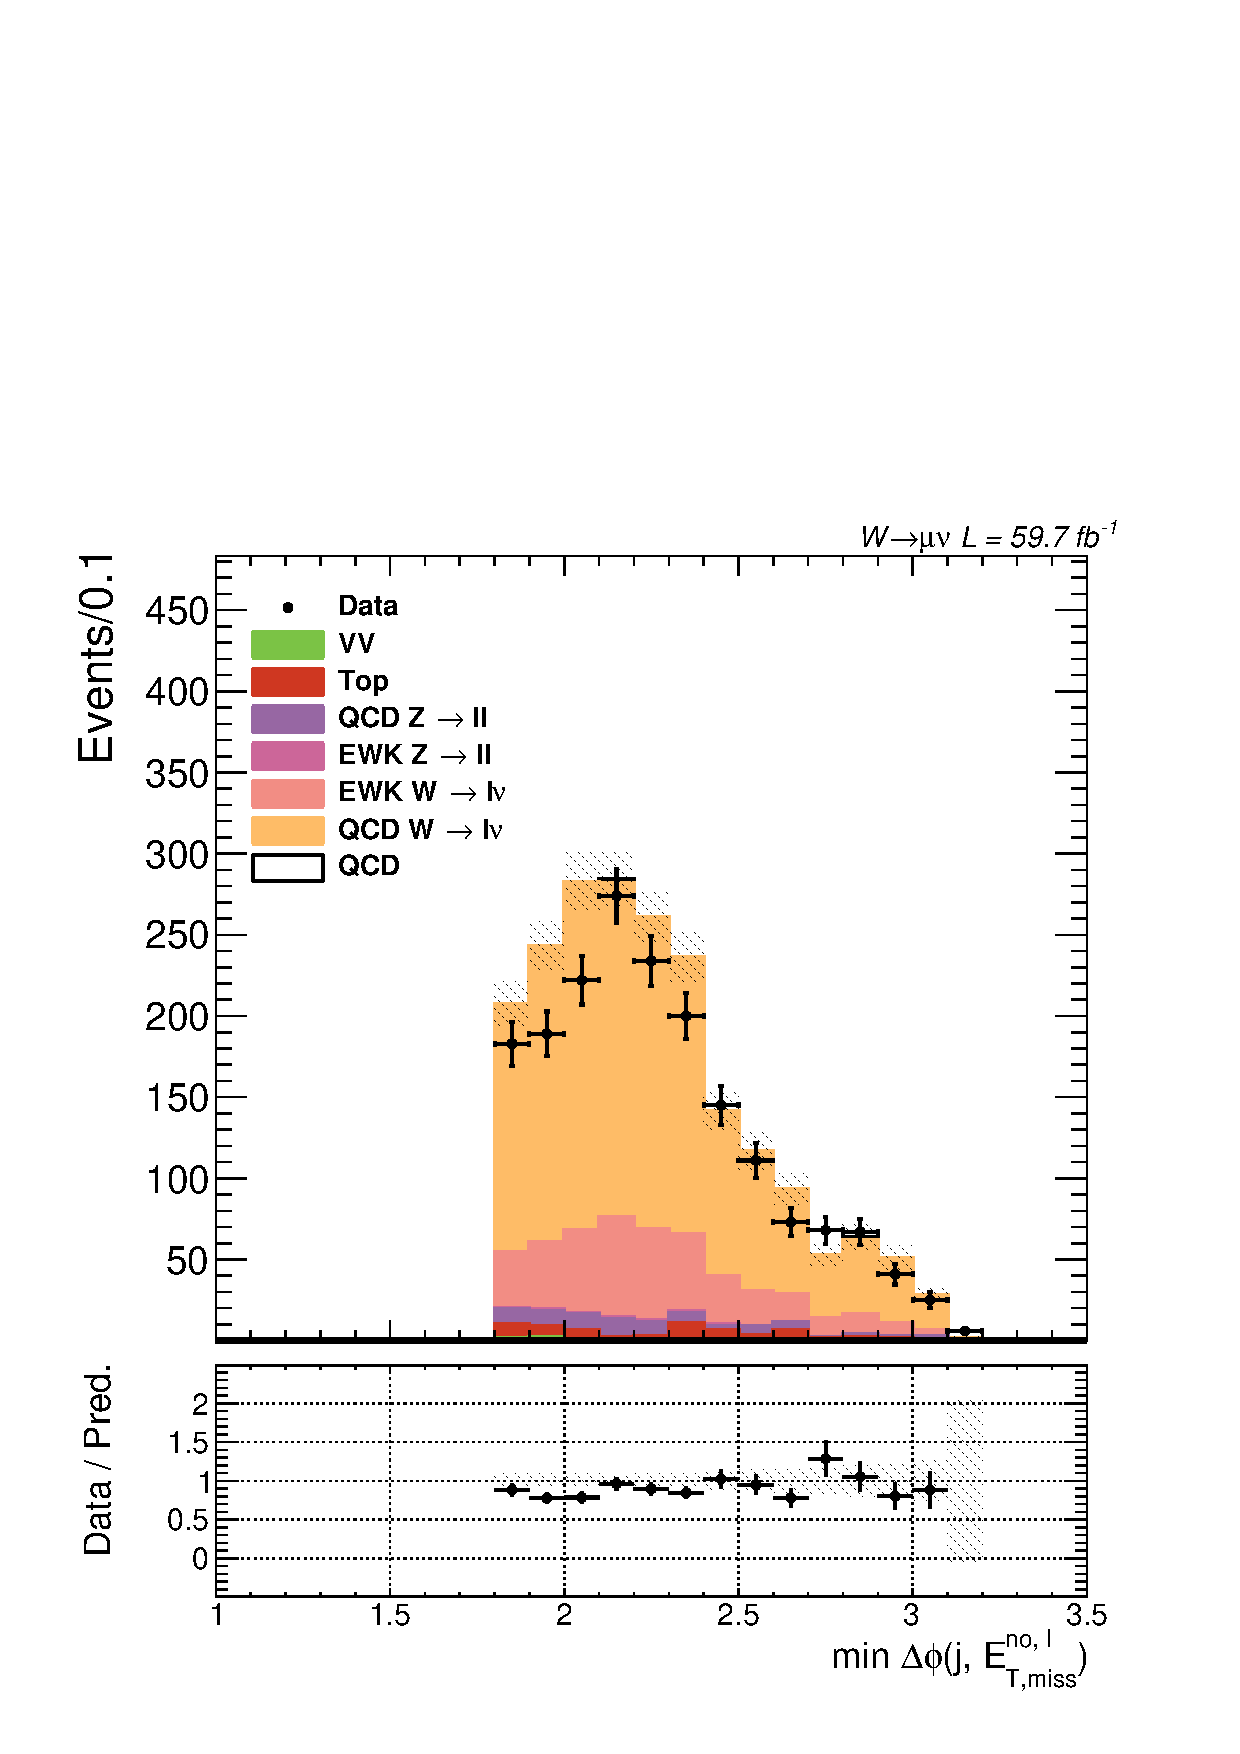
\includegraphics[width=0.49\textwidth]{Control_Regions/2018_VTR/Wmunu/MetNoLep_CleanJet_mindPhi.pdf}
    }
  \caption{Distributions of $M_{T,\mu}$ and \mindphinomu variables in single muon region for MTR (top) and VTR (bottom) categories for the 2018 era of data taking.}
  \label{fig:2018_Wmunu_2}
\end{figure}

\newpage



\hspace{10pt} Similarly to the double muon region, the single muon region is not affected by the HEM issue in 2018 due to the tight muon requirement. Figures [A.R] confirms these claims by showing no significant excess in the affected $(\eta, \phi)$ range. The following sections are going to introduce electron regions where, for the single electron case, this effect will require special attention.

\subsection{Double Electron CR}
\hspace{10pt} The first step, when adapting the double lepton region structure for the purposes of the electron case, is to modify the electron veto from the SR forming selection requirements. The choice of electrons requires exactly two electrons in the event, at least one of which needs to satisfy tight requirements, while both of them have to follow the $p_T>$~40/10~GeV thresholds for the leading/subleading electron respectively. Upon selecting the objects, the dilepton mass requirement of 60$~<m_{ll}<~$120~GeV is applied.

\hspace{10pt} Figures~\ref{fig:2017_Zee_1} and~\ref{fig:2017_Zee_2} show the $m_{jj}$ and $m_{ll}$ distributions for both categories and both eras of data taking. The $m_{jj}$ variable shows a good level of agreement between data and simulation. Additionally, Figures~\ref{fig:2017_Zee_2} and~\ref{fig:2018_Zee_2} show the data to prediction agreement for the \mindphinoe~and $E_{T, miss}^{no, e}$. The latter is defined in the same way as its muon counterpart, by eliminating the contribution from the electron objects when computing it.

\hspace{10pt} As it was the case for the double muon region, this region is unaffected by the HEM problem in 2018 due to very tight requirements in the form of the electron identification and the dilepton mass. The previous reasoning also accounts for the lack of contribution originating from QCD multijet processes.

\begin{figure}[htbp]
  \centering
    \subfigure[$m_{ll}$ - MTR]{
    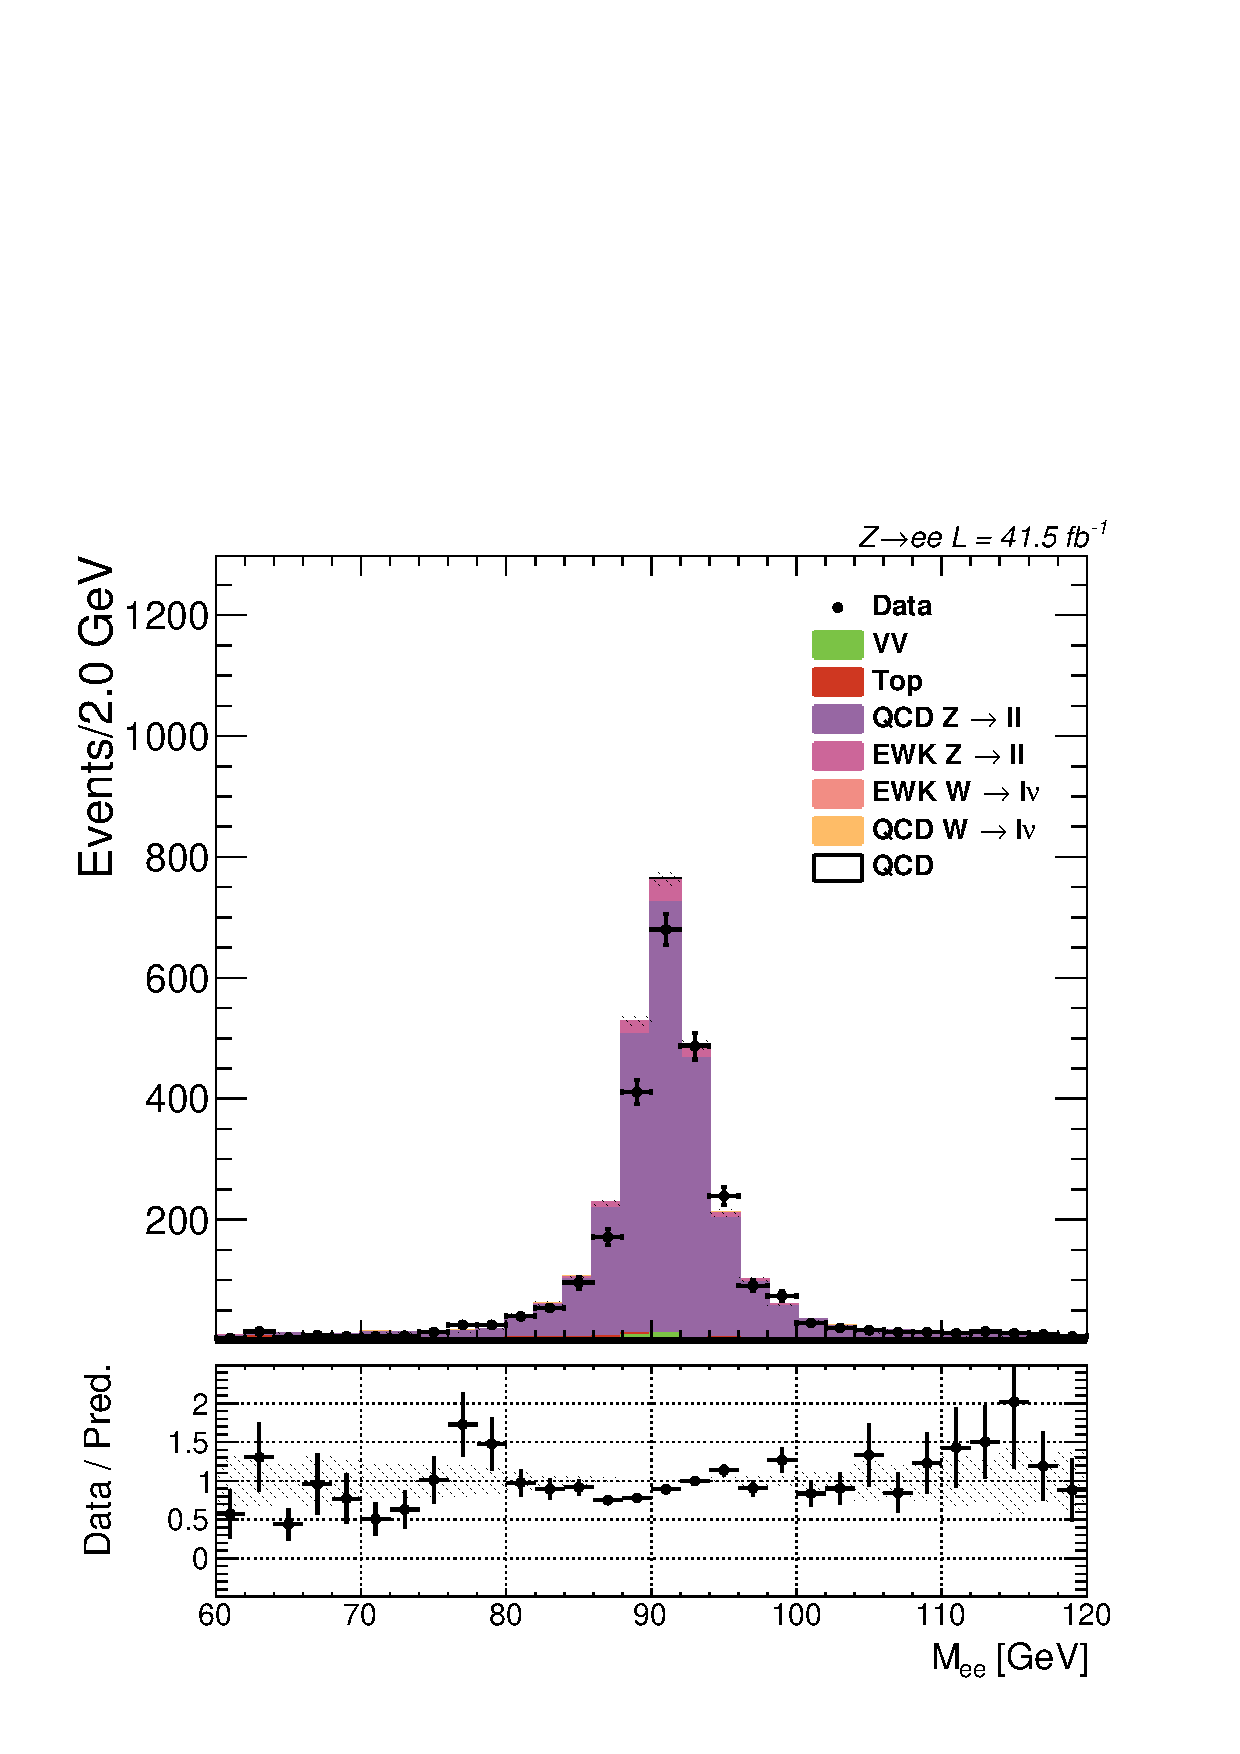
\includegraphics[width=0.49\textwidth]{Control_Regions/2017_MTR/Zee/diElectron_mass.pdf}
    }
    \subfigure[$m_{jj}$ - MTR]{
    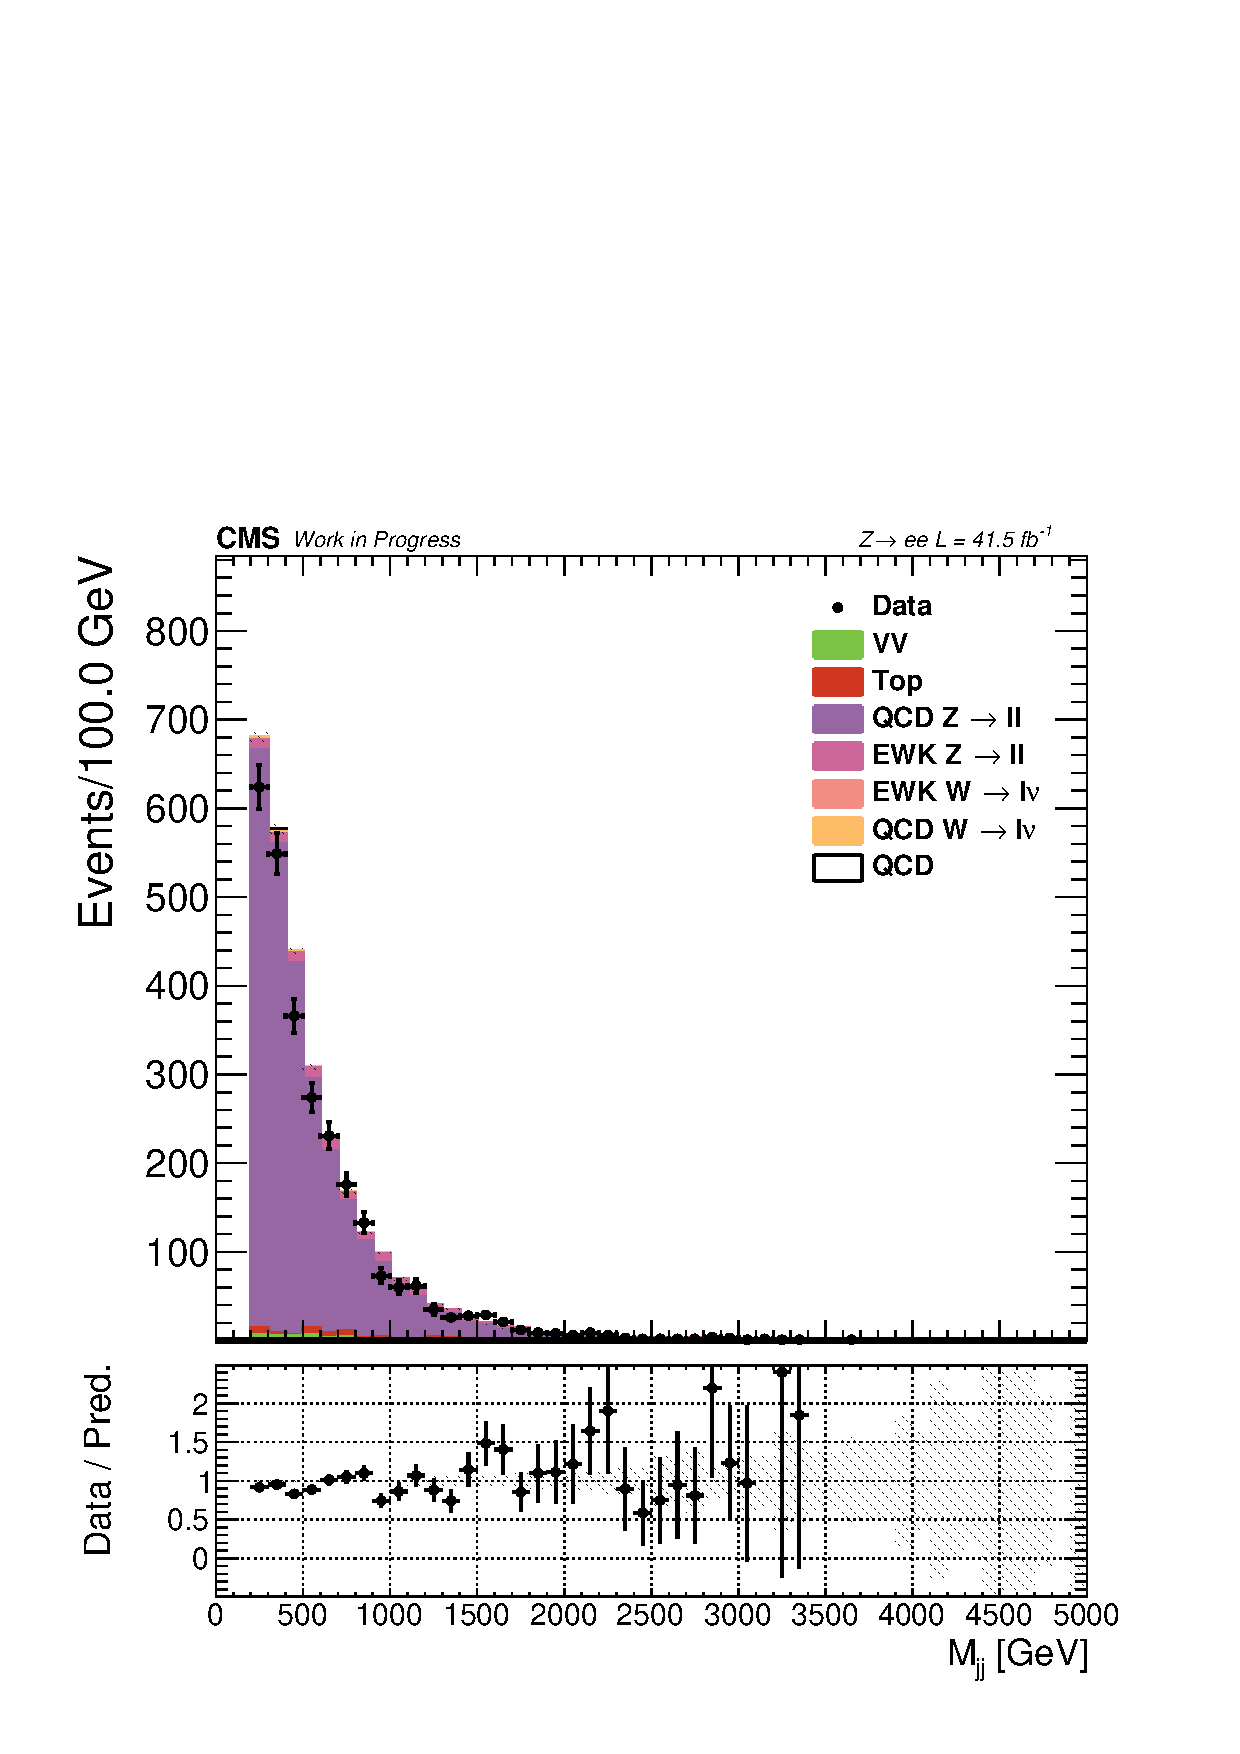
\includegraphics[width=0.49\textwidth]{Control_Regions/2017_MTR/Zee/leadingJet_mjj.pdf}
    }
\\
    \subfigure[$m_{ll}$ - VTR]{
    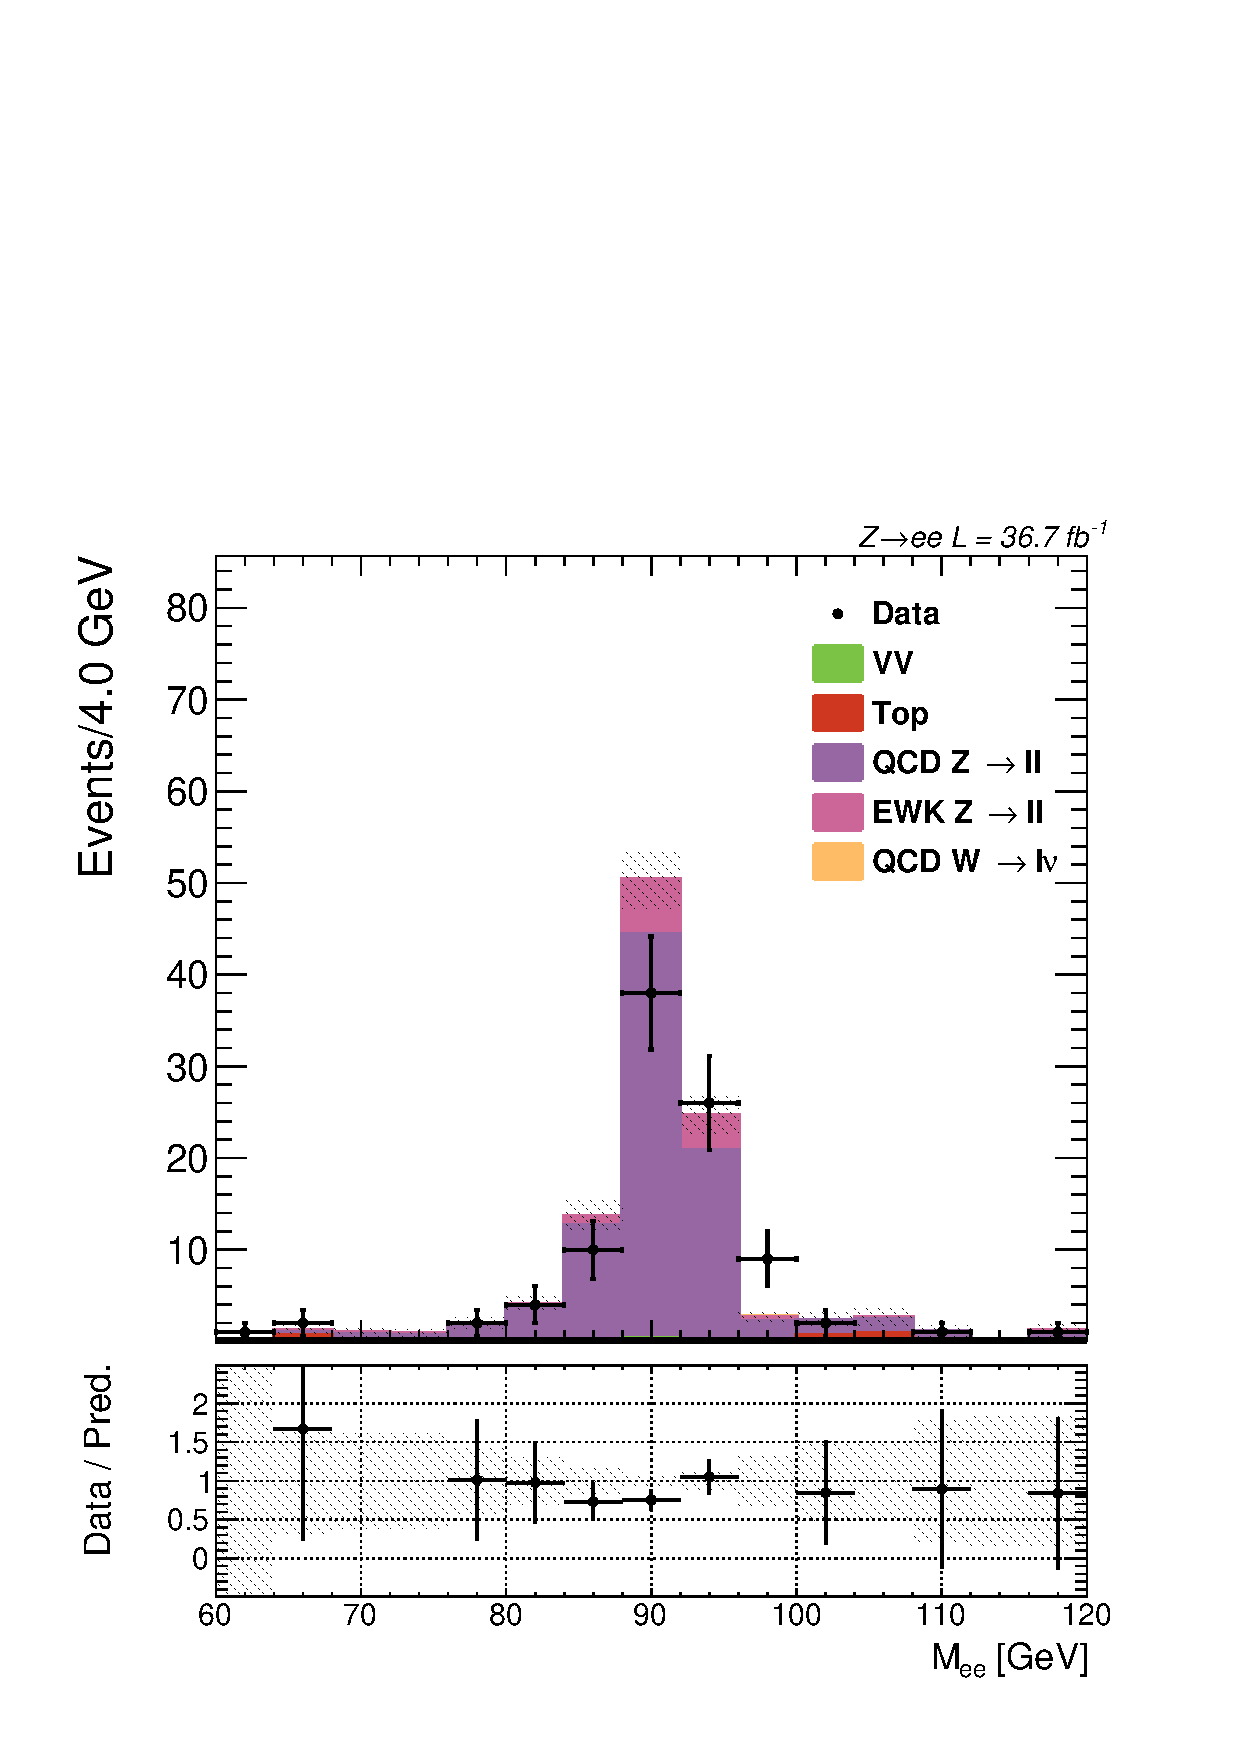
\includegraphics[width=0.49\textwidth]{Control_Regions/2017_VTR/Zee/diElectron_mass.pdf}
    }
    \subfigure[$m_{jj}$ - VTR]{
    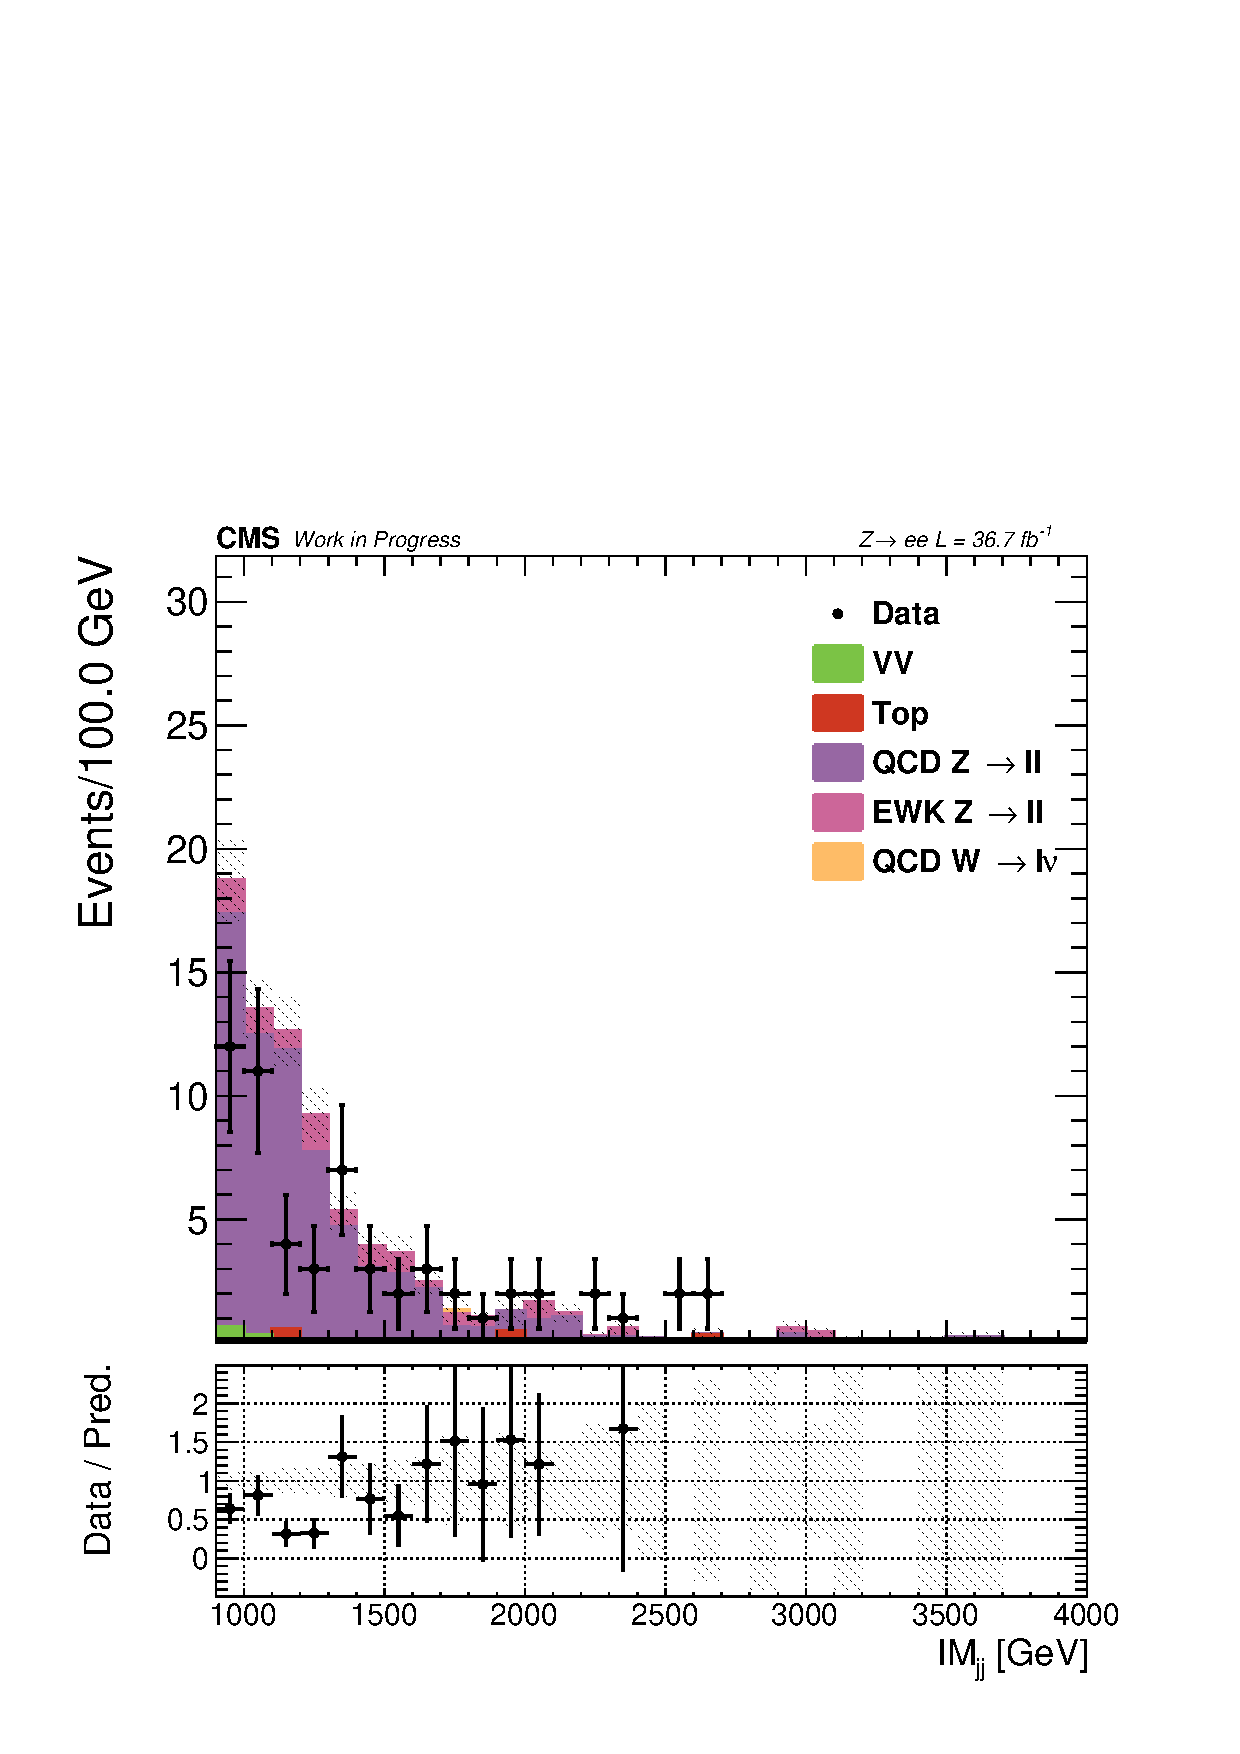
\includegraphics[width=0.49\textwidth]{Control_Regions/2017_VTR/Zee/lMjj.pdf}
    }
  \caption{Distributions of $m_{ll}$ and $m_{jj}$ variables in double muon region for MTR (top) and VTR (bottom) categories for the 2017 era of data taking.}
  \label{fig:2017_Zee_1}
\end{figure}

\begin{figure}[htbp]
  \centering
    \subfigure[$m_{ll}$ - MTR]{
    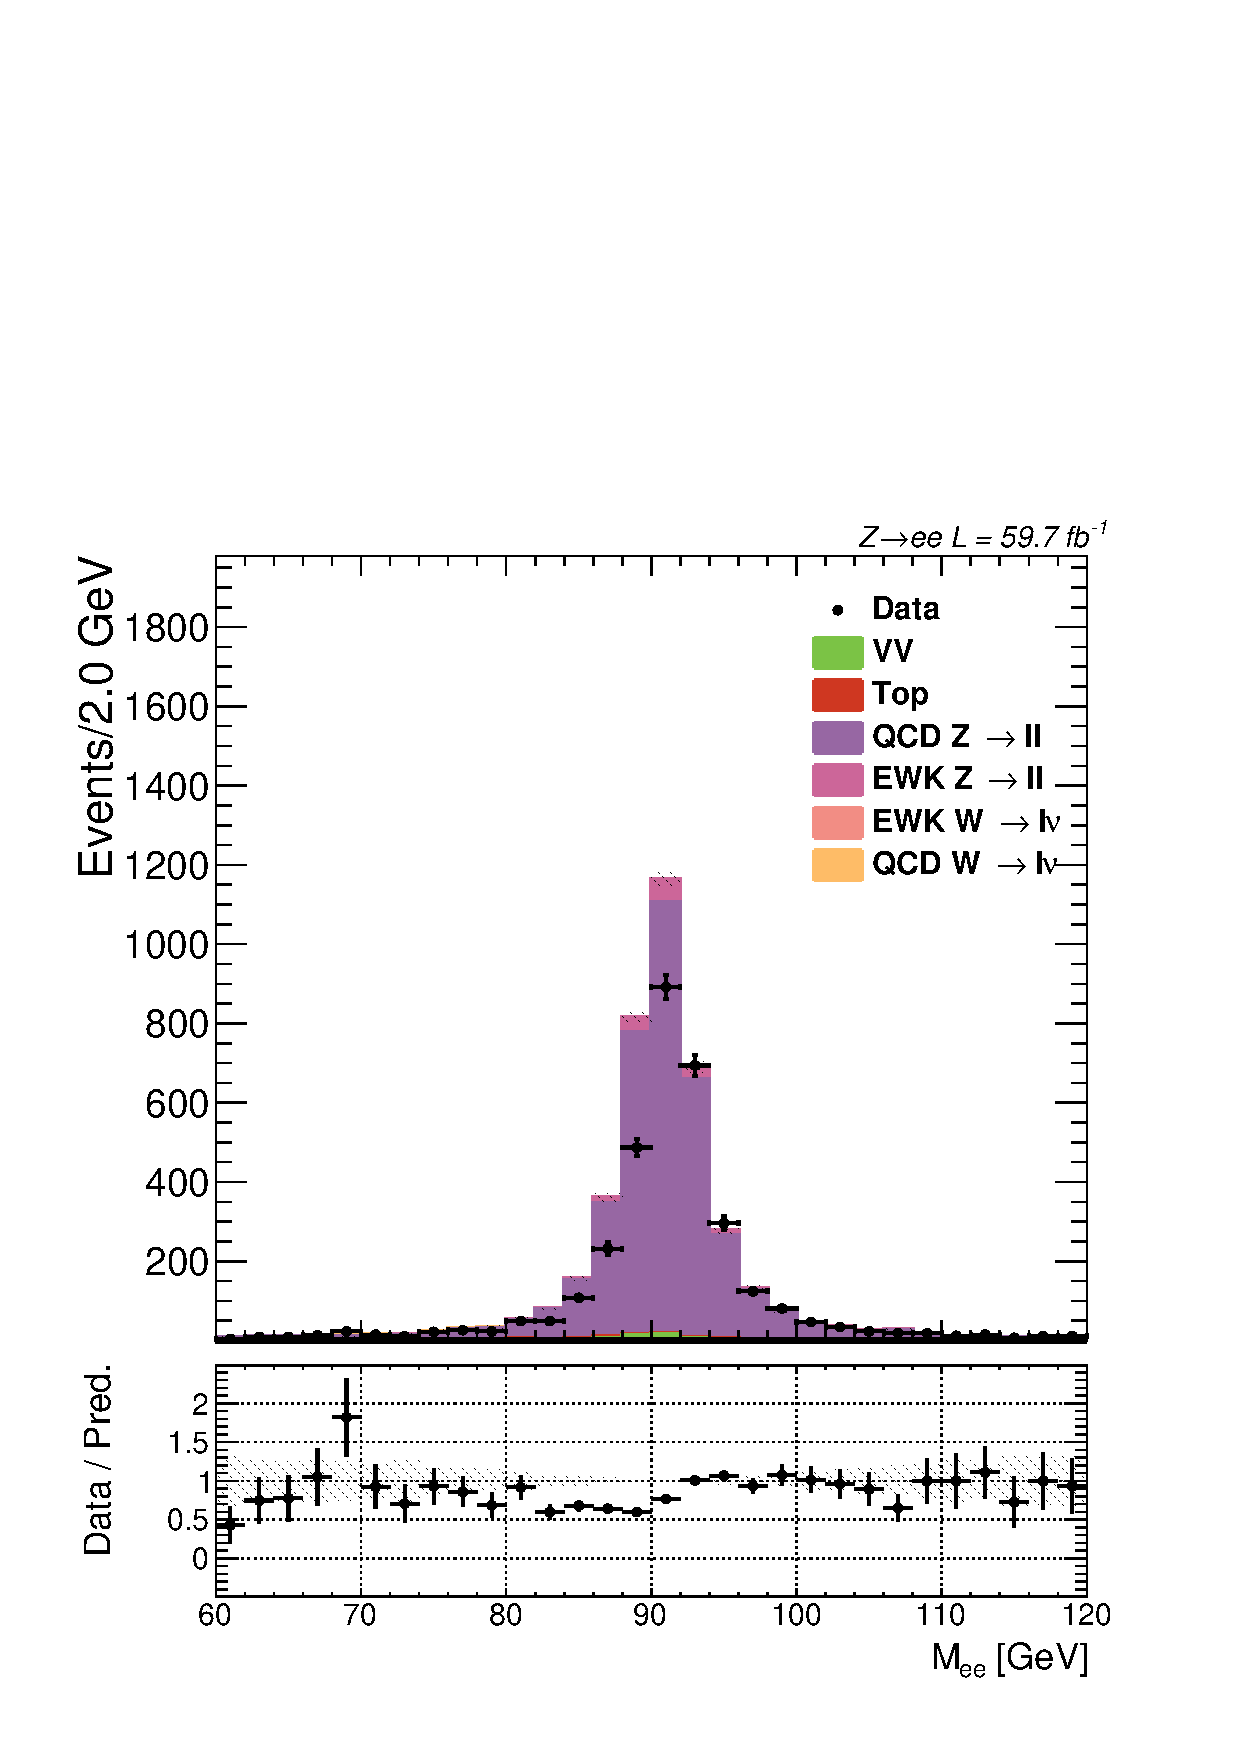
\includegraphics[width=0.49\textwidth]{Control_Regions/2018_MTR/Zee/diElectron_mass.pdf}
    }
    \subfigure[$m_{jj}$ - MTR]{
    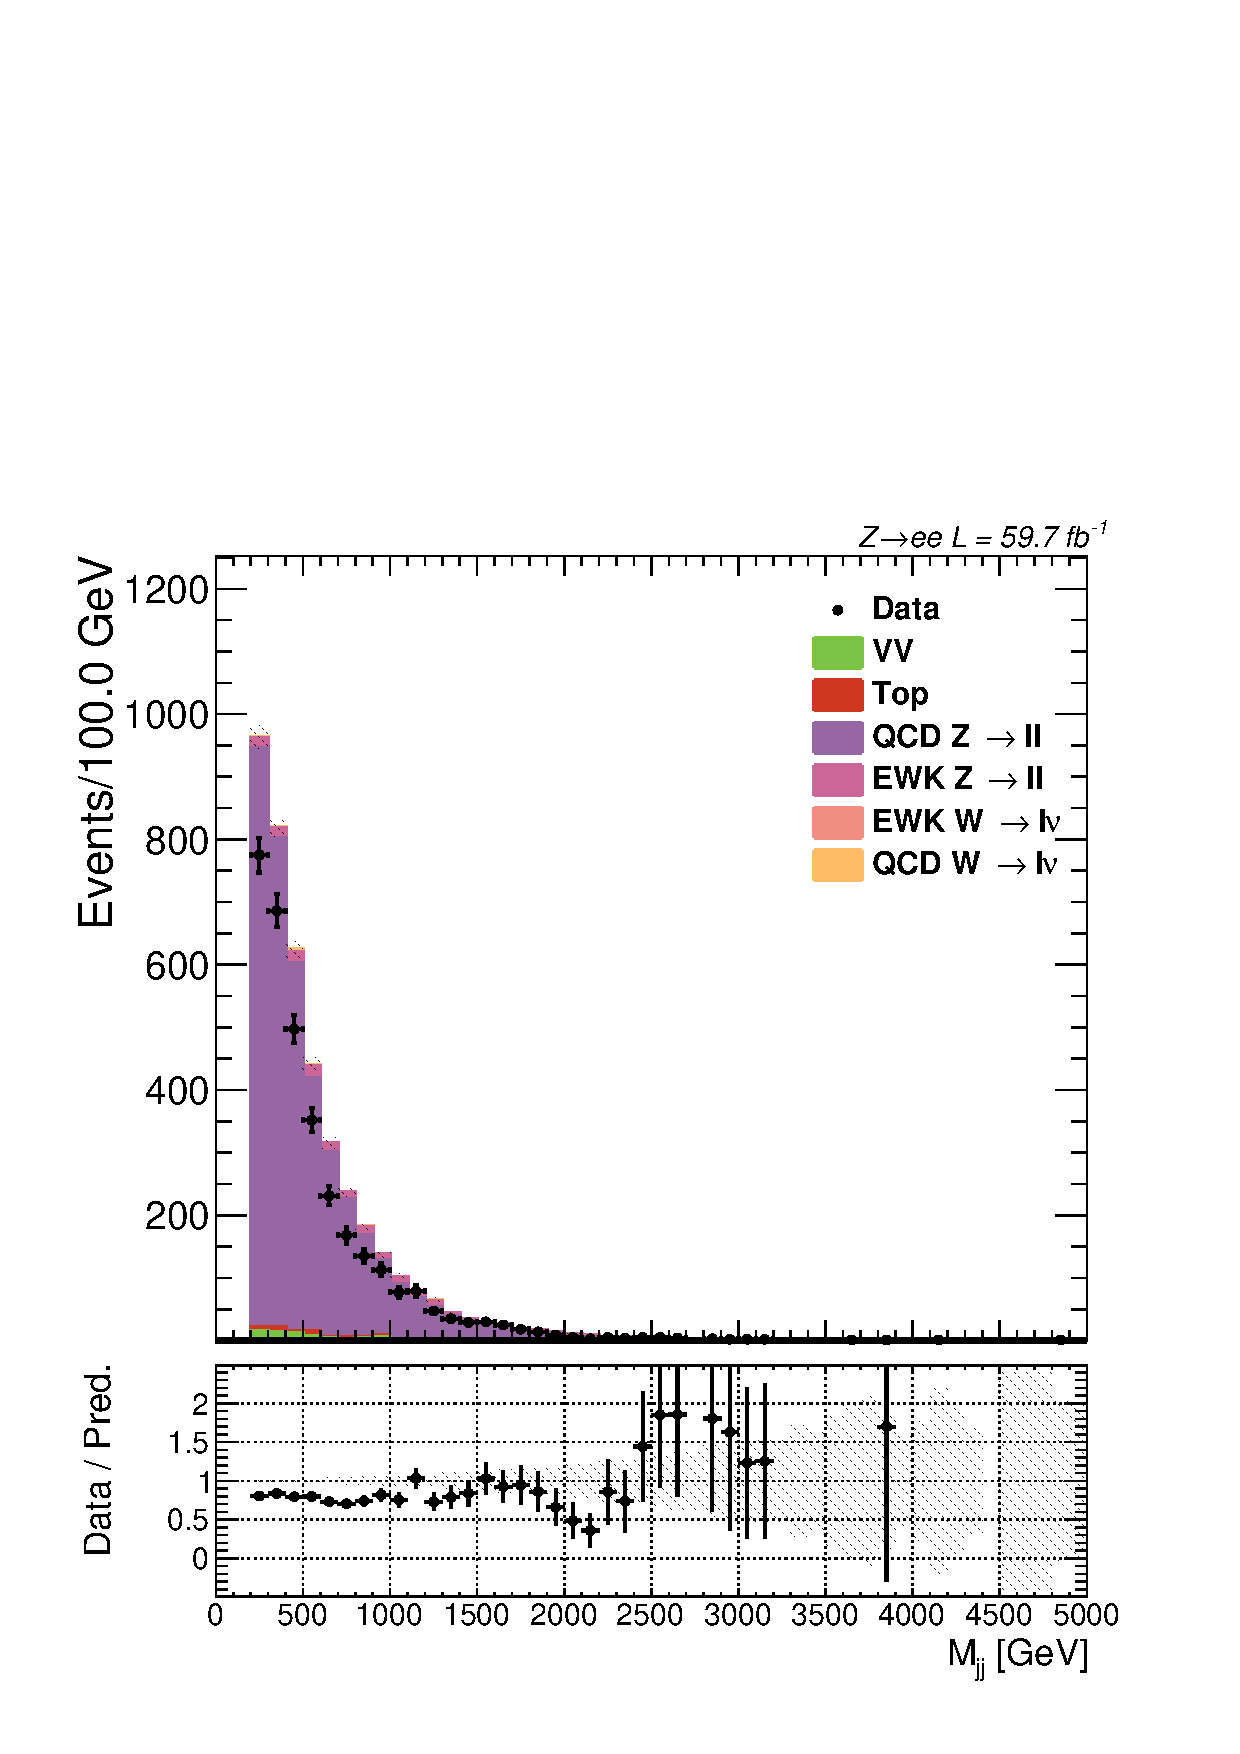
\includegraphics[width=0.49\textwidth]{Control_Regions/2018_MTR/Zee/leadingJet_mjj.pdf}
    }\\
    \subfigure[$m_{ll}$ - VTR]{
    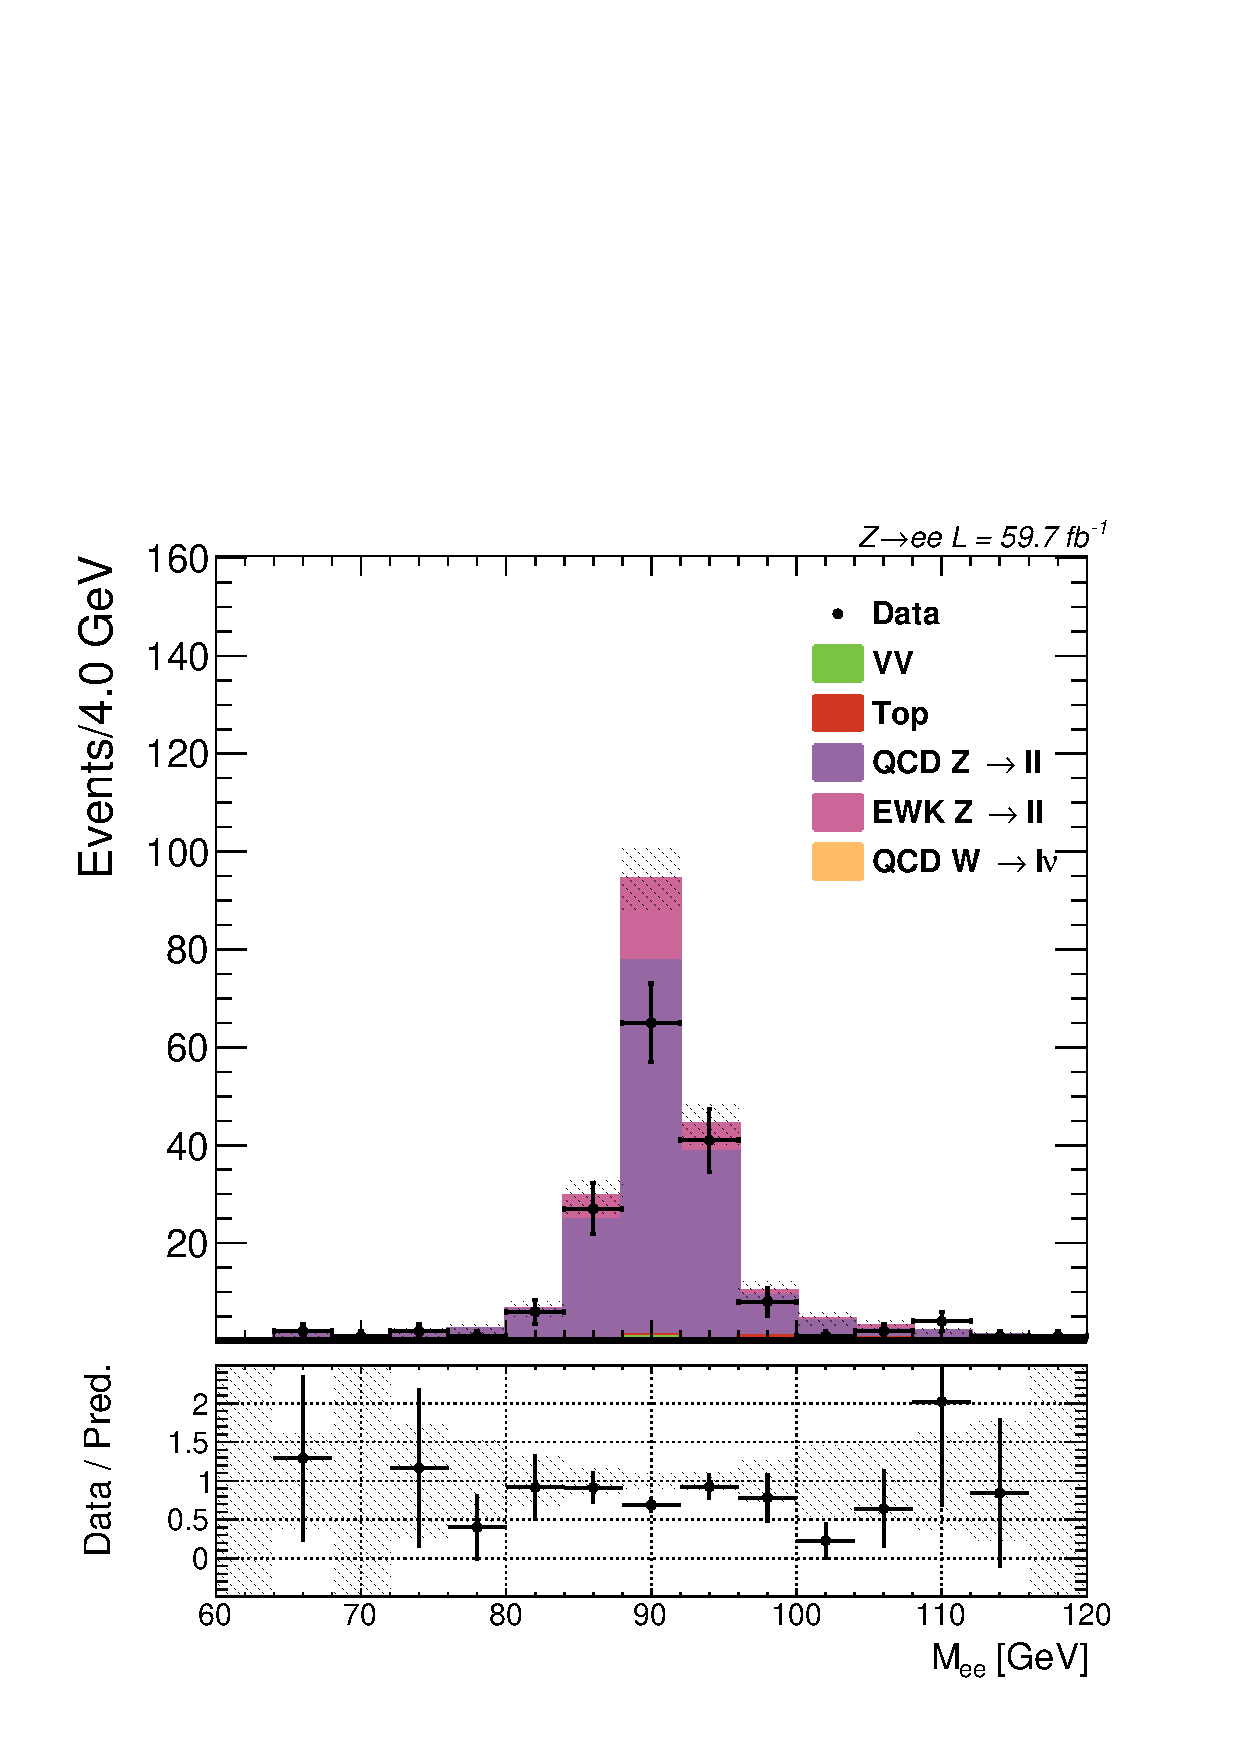
\includegraphics[width=0.49\textwidth]{Control_Regions/2018_VTR/Zee/diElectron_mass.pdf}
    }
    \subfigure[$m_{jj}$ - VTR]{
    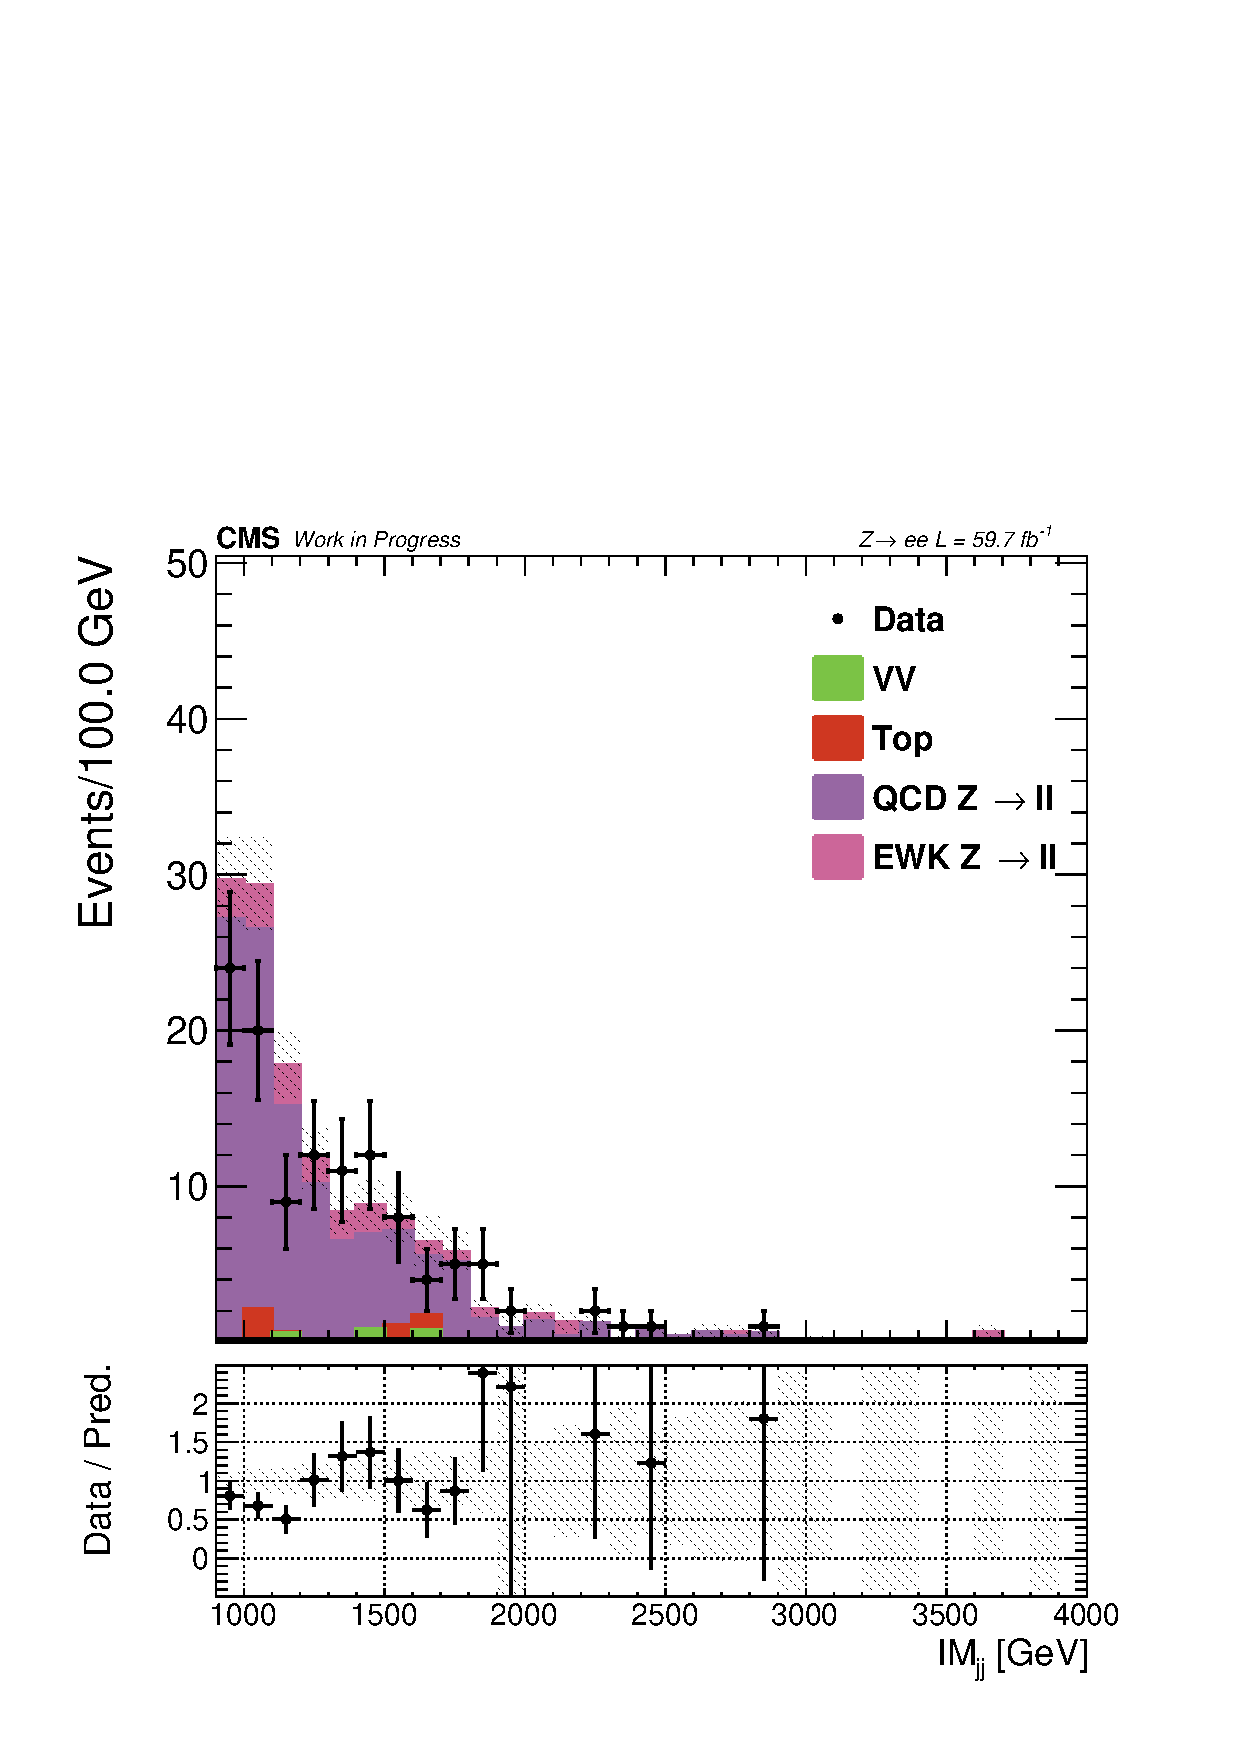
\includegraphics[width=0.49\textwidth]{Control_Regions/2018_VTR/Zee/lMjj.pdf}
    }
  \caption{Distributions of $m_{jj}$ and $m_{ll}$ variables in double muon region for MTR (top) and VTR (bottom) categories for the 2018 era of data taking.}
  \label{fig:2018_Zee_1}
\end{figure}


\begin{figure}[htbp]
  \centering
    \subfigure[$E_{T,miss}$ - MTR]{
    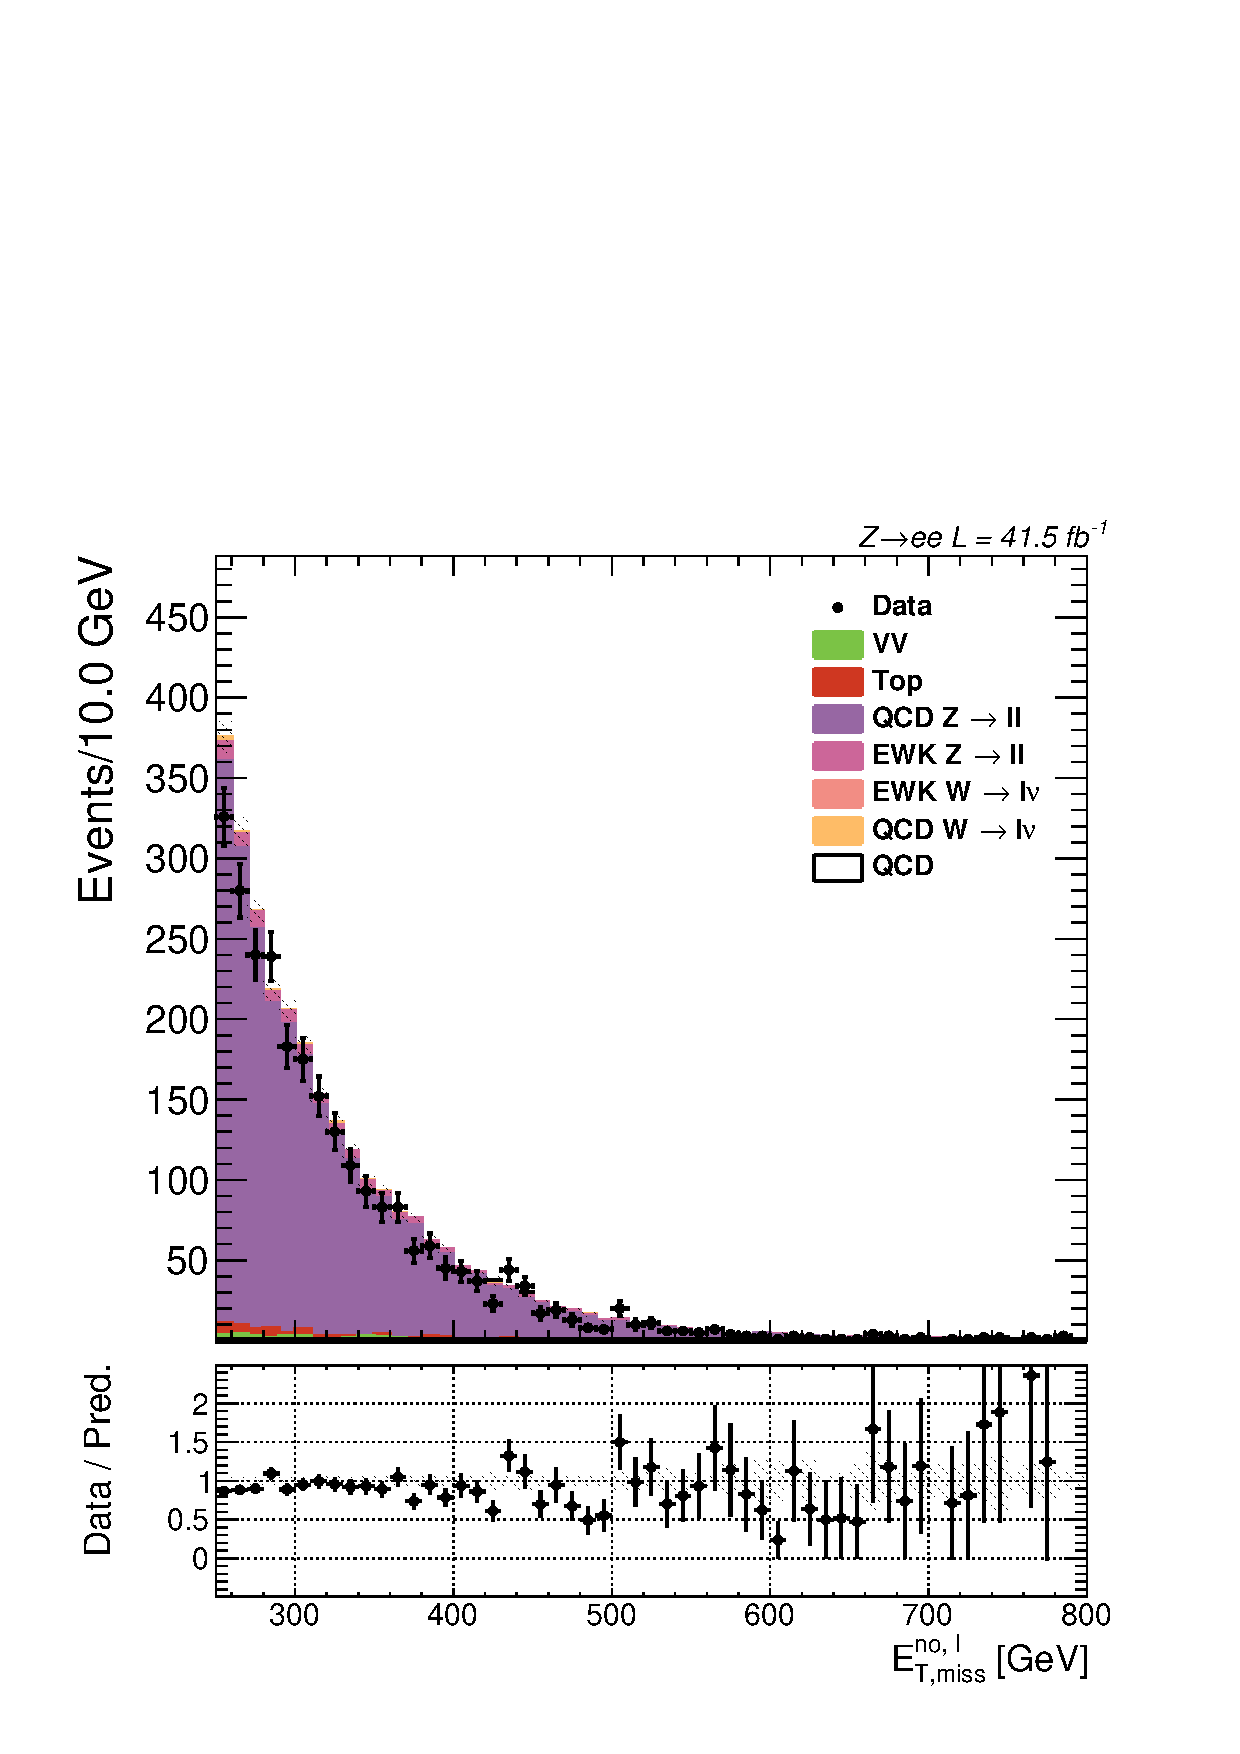
\includegraphics[width=0.49\textwidth]{Control_Regions/2017_MTR/Zee/MetNoMu.pdf}
    }
    \subfigure[$min\Delta\phi(j,E_{T,miss})$ - MTR]{
    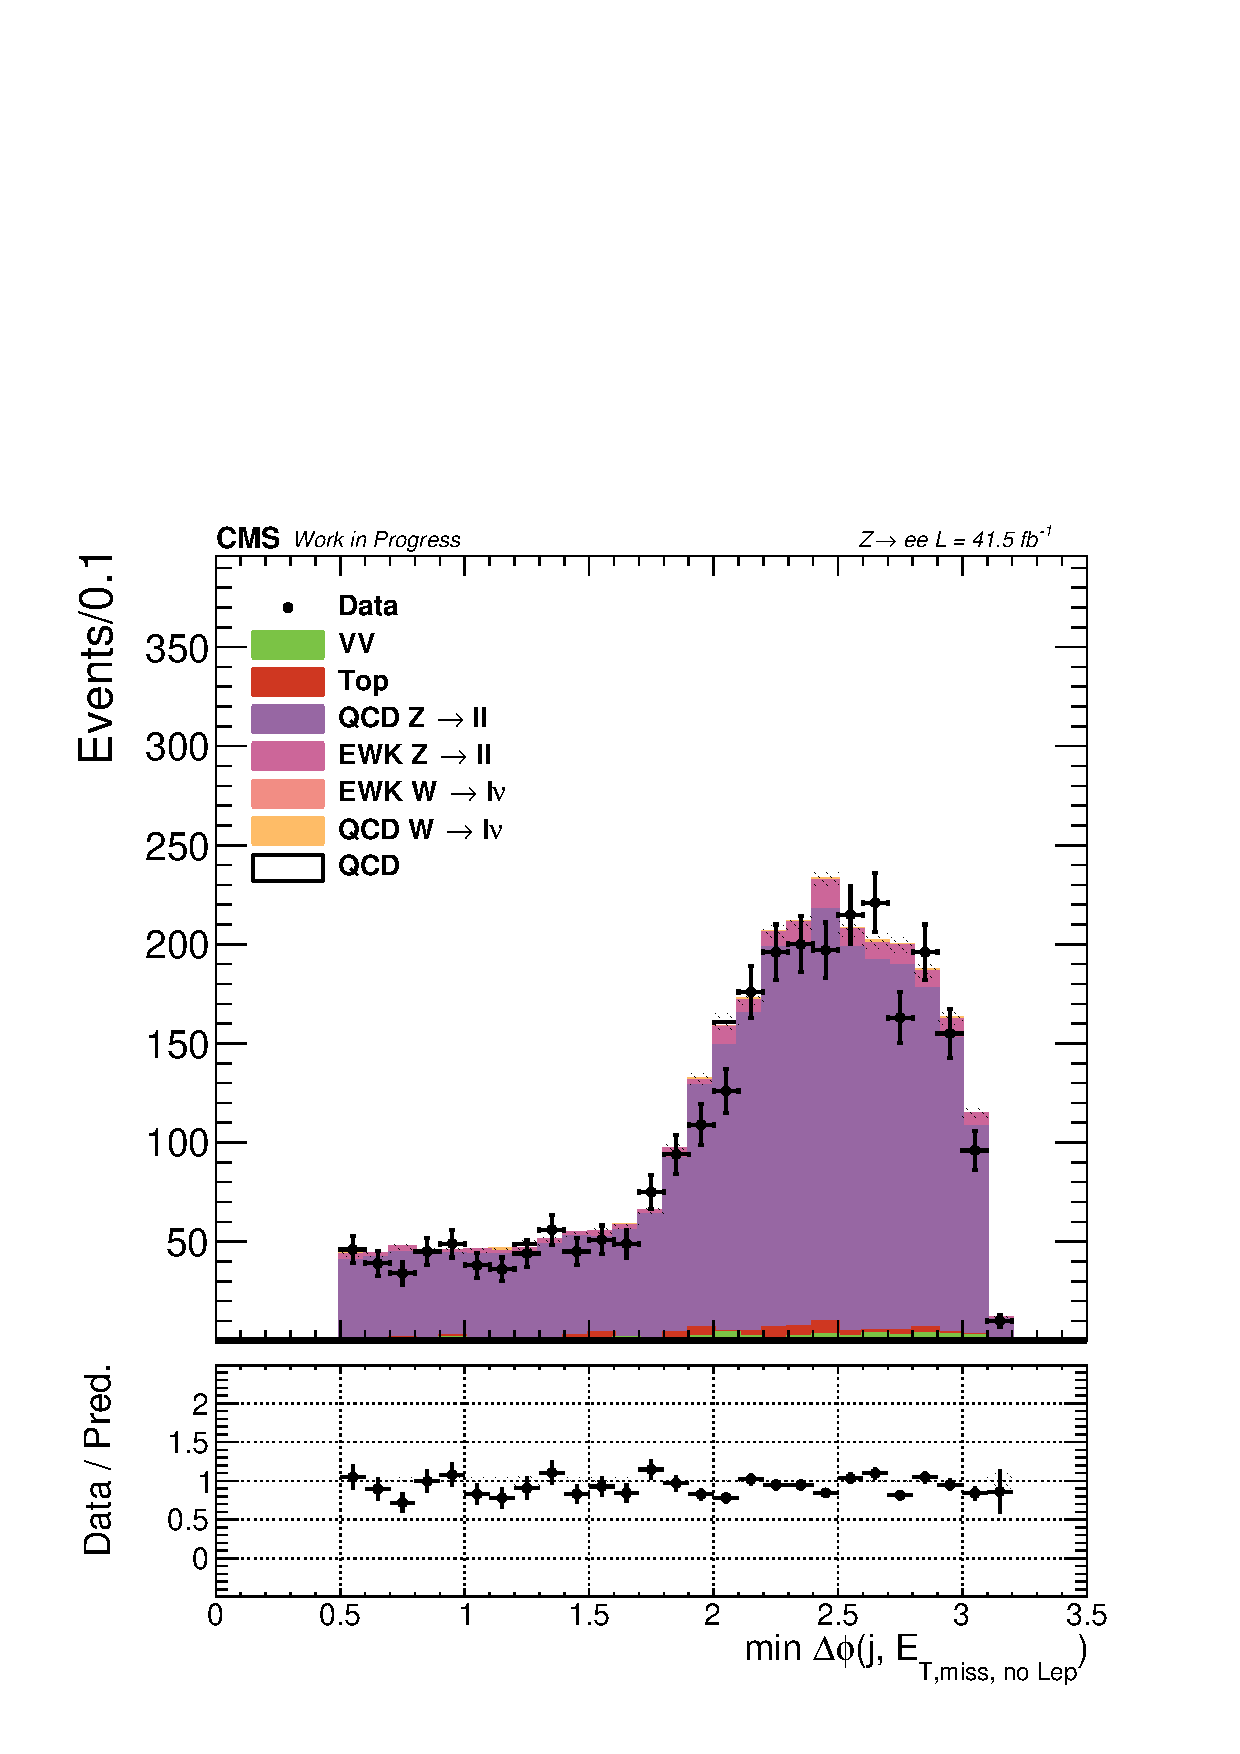
\includegraphics[width=0.49\textwidth]{Control_Regions/2017_MTR/Zee/MetNoLep_CleanJet_mindPhi.pdf}
    }\\
    \subfigure[$E_{T,miss}$ - VTR]{
    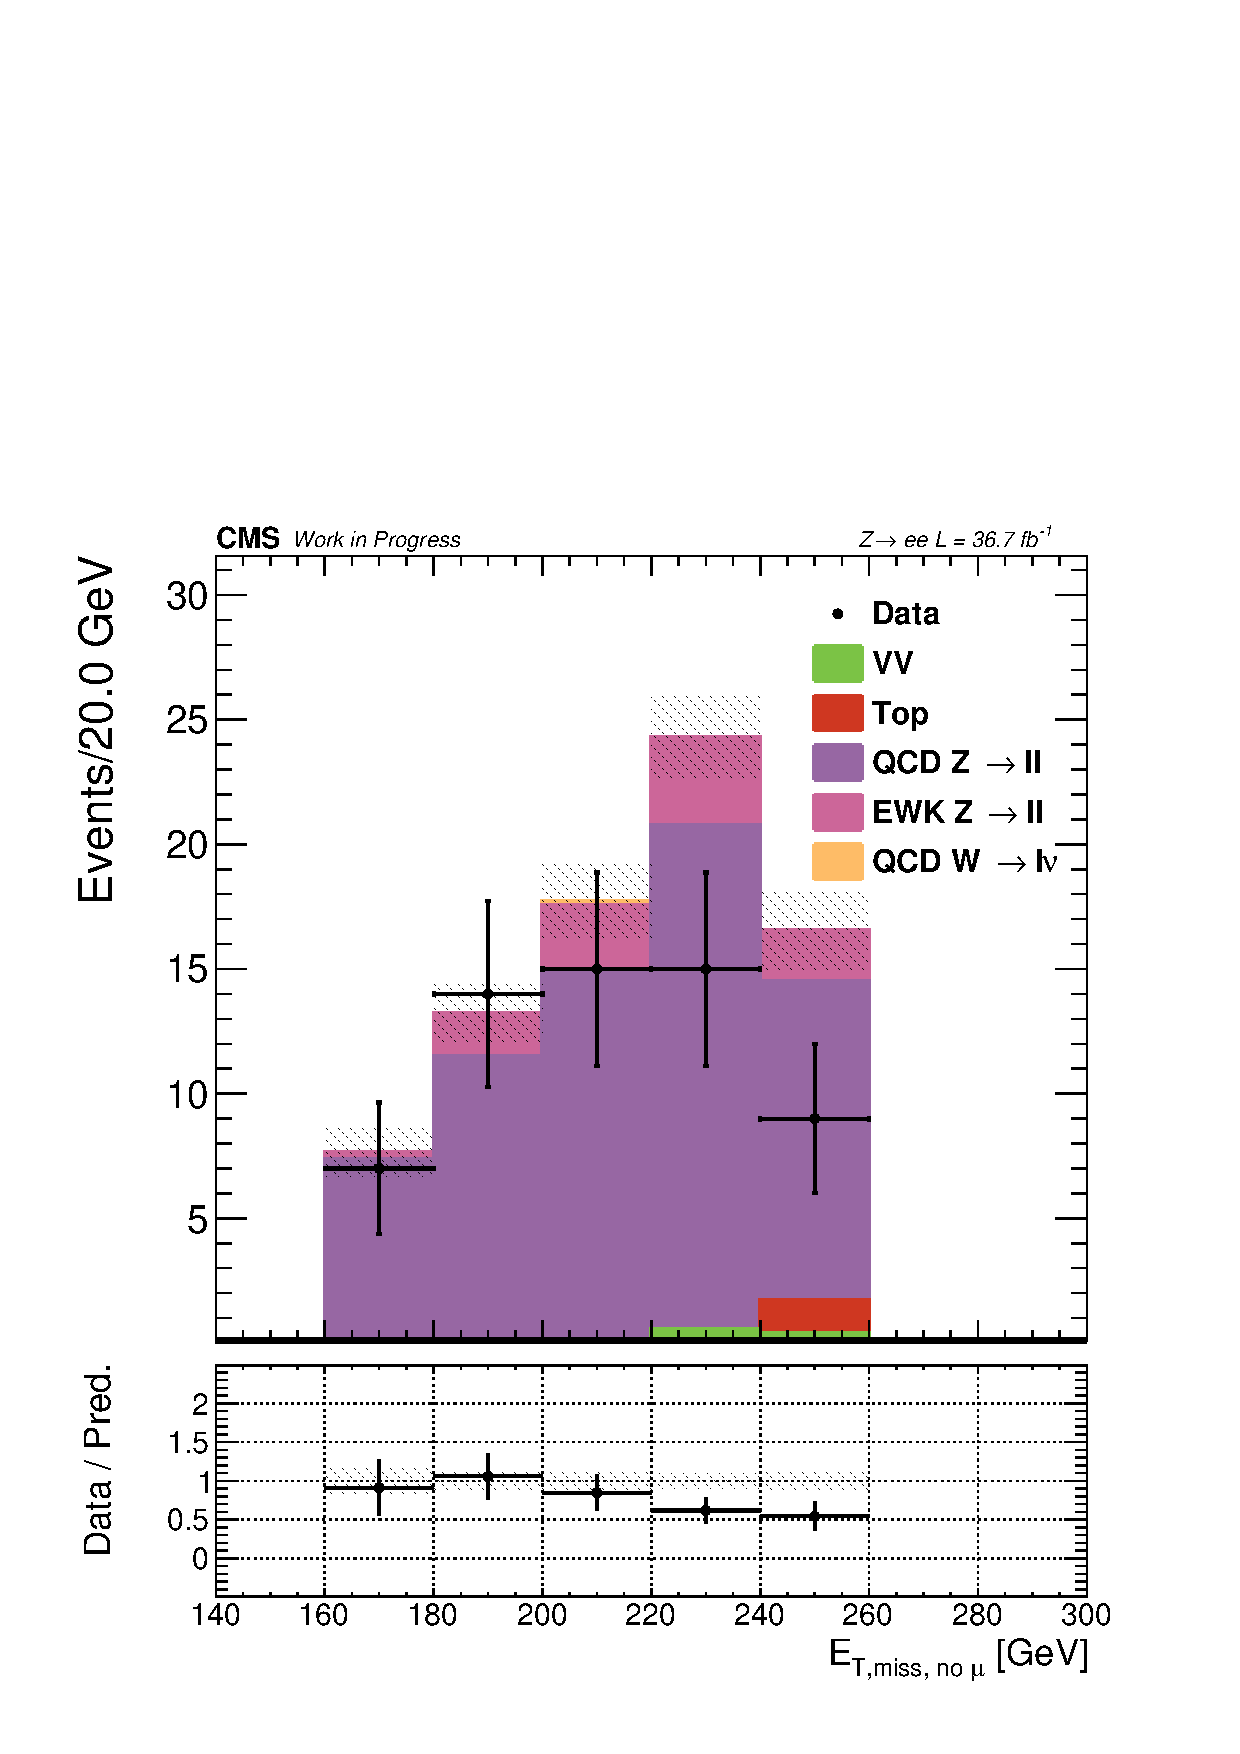
\includegraphics[width=0.49\textwidth]{Control_Regions/2017_VTR/Zee/MetNoMu.pdf}
    }
    \subfigure[$min\Delta\phi(j,E_{T,miss})$ - VTR]{
    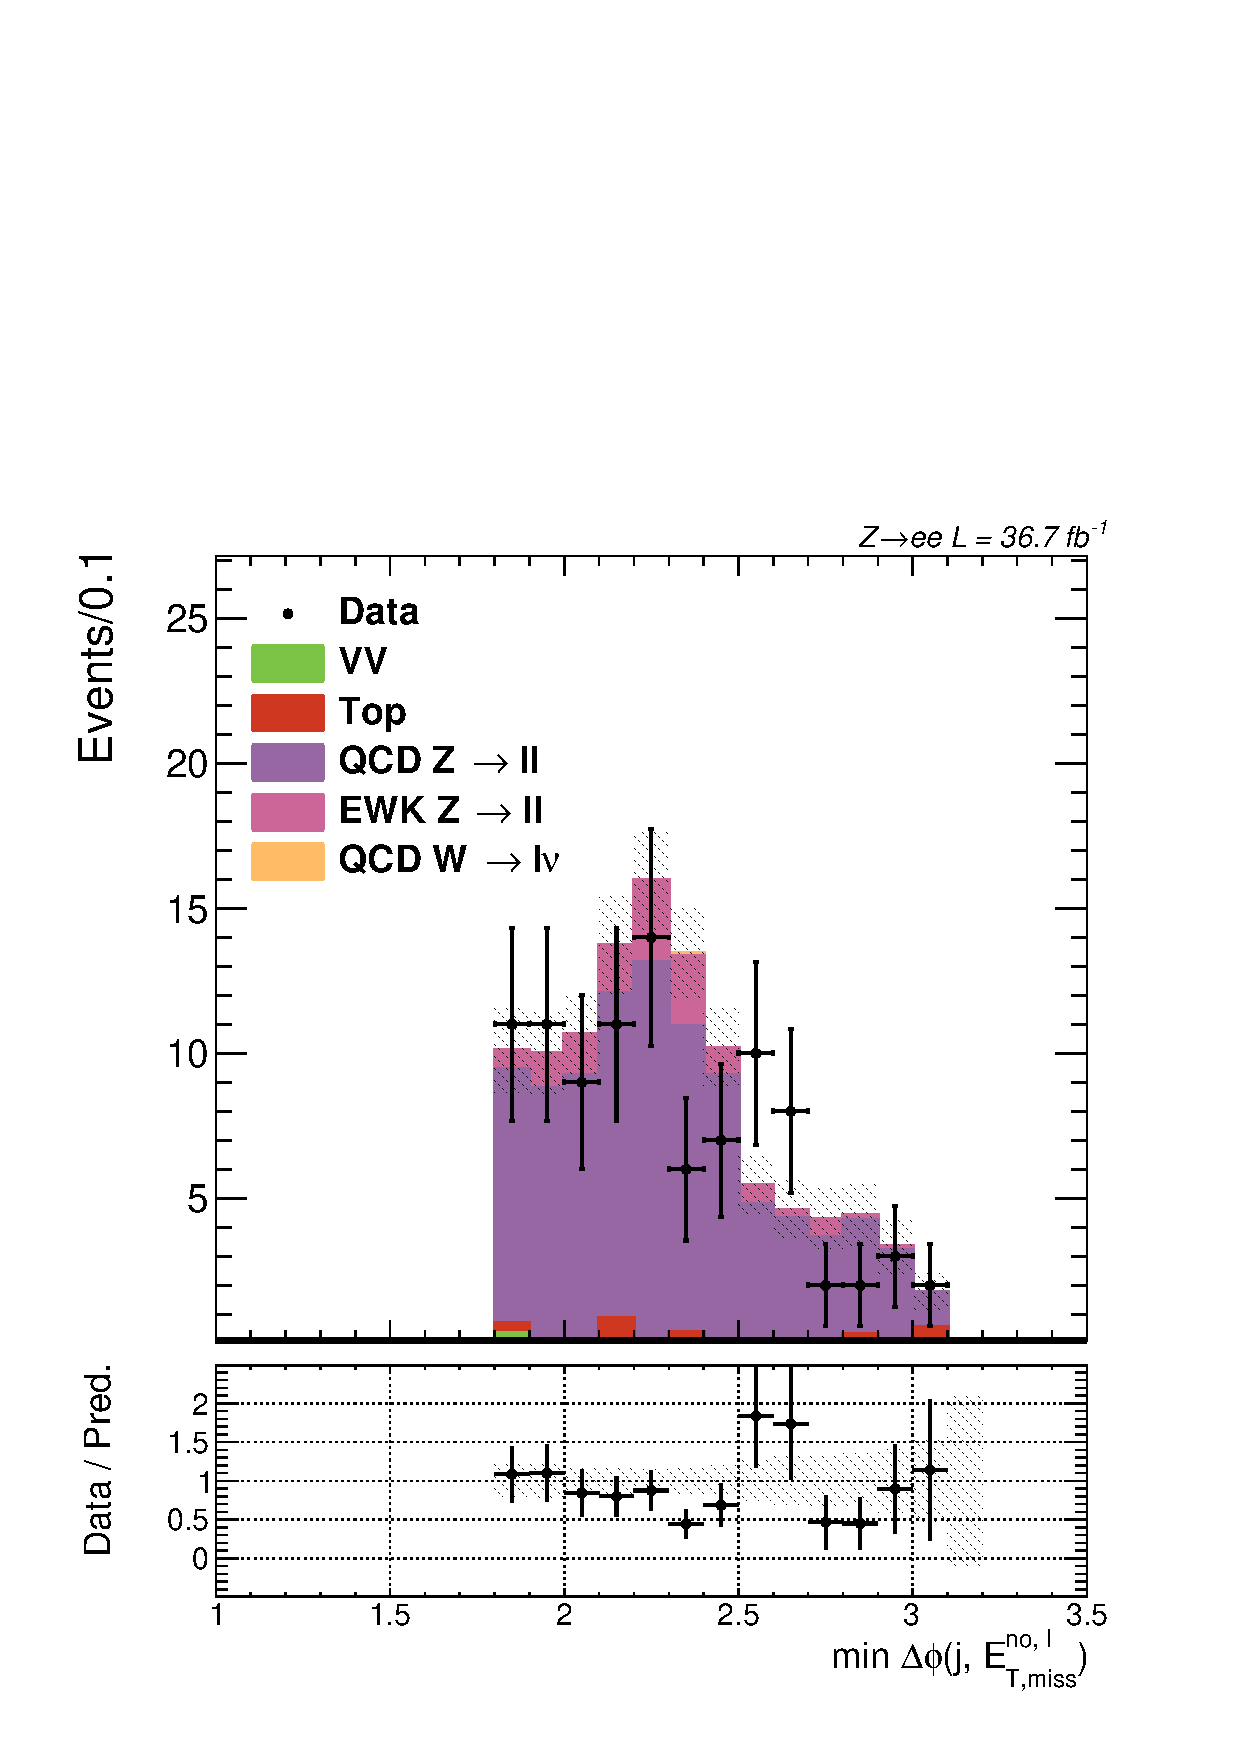
\includegraphics[width=0.49\textwidth]{Control_Regions/2017_VTR/Zee/MetNoLep_CleanJet_mindPhi.pdf}
    }
  \caption{Distributions of $E_{T,miss}$ and $min\Delta\phi(j,E_{T,miss})$ variables in the double muon region for MTR (top) and VTR (bottom) categories for the 2017 era of data taking.}
  \label{fig:2017_Zee_2}
\end{figure}


\begin{figure}[htbp]
  \centering
    \subfigure[$E_{T,miss}$ - MTR]{
    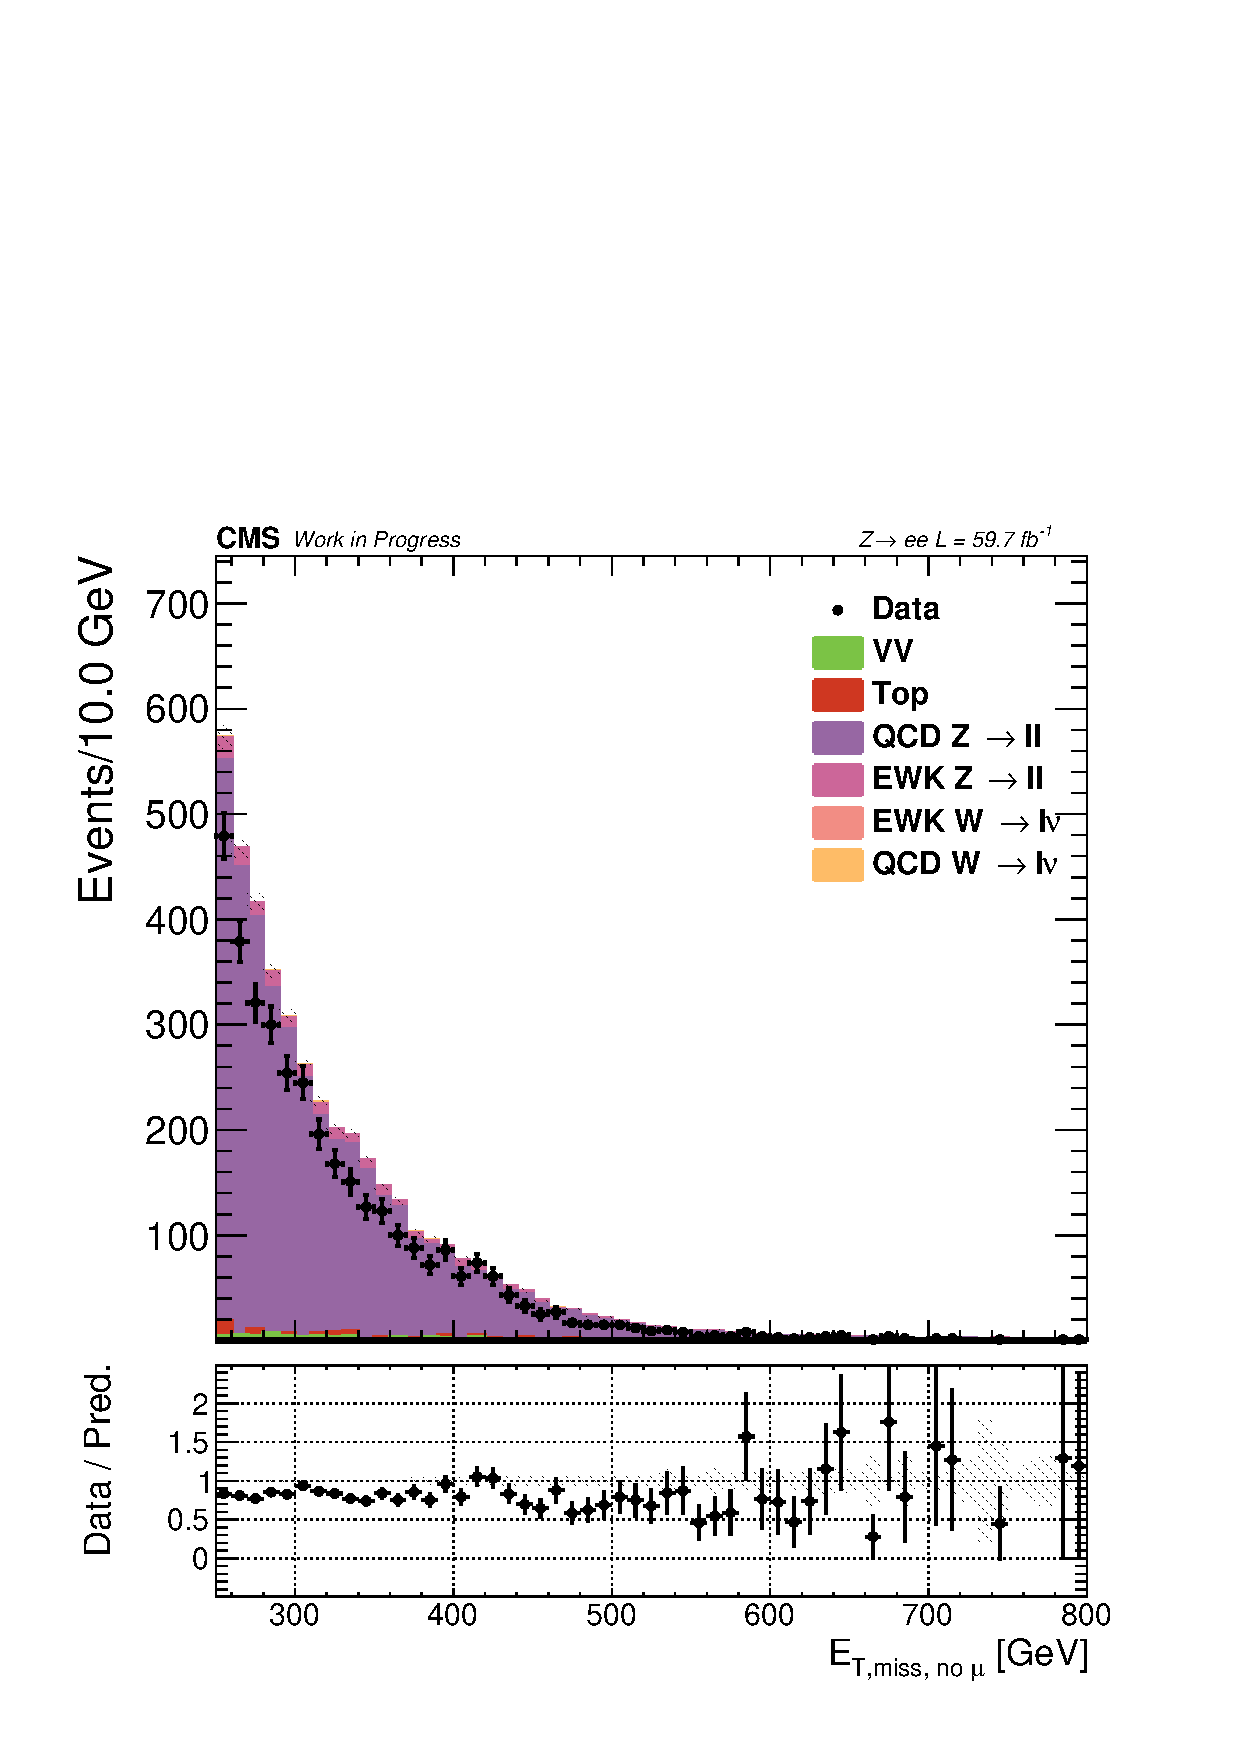
\includegraphics[width=0.49\textwidth]{Control_Regions/2018_MTR/Zee/MetNoMu.pdf}
    }
    \subfigure[$min\Delta\phi(j,E_{T,miss})$ - MTR]{
    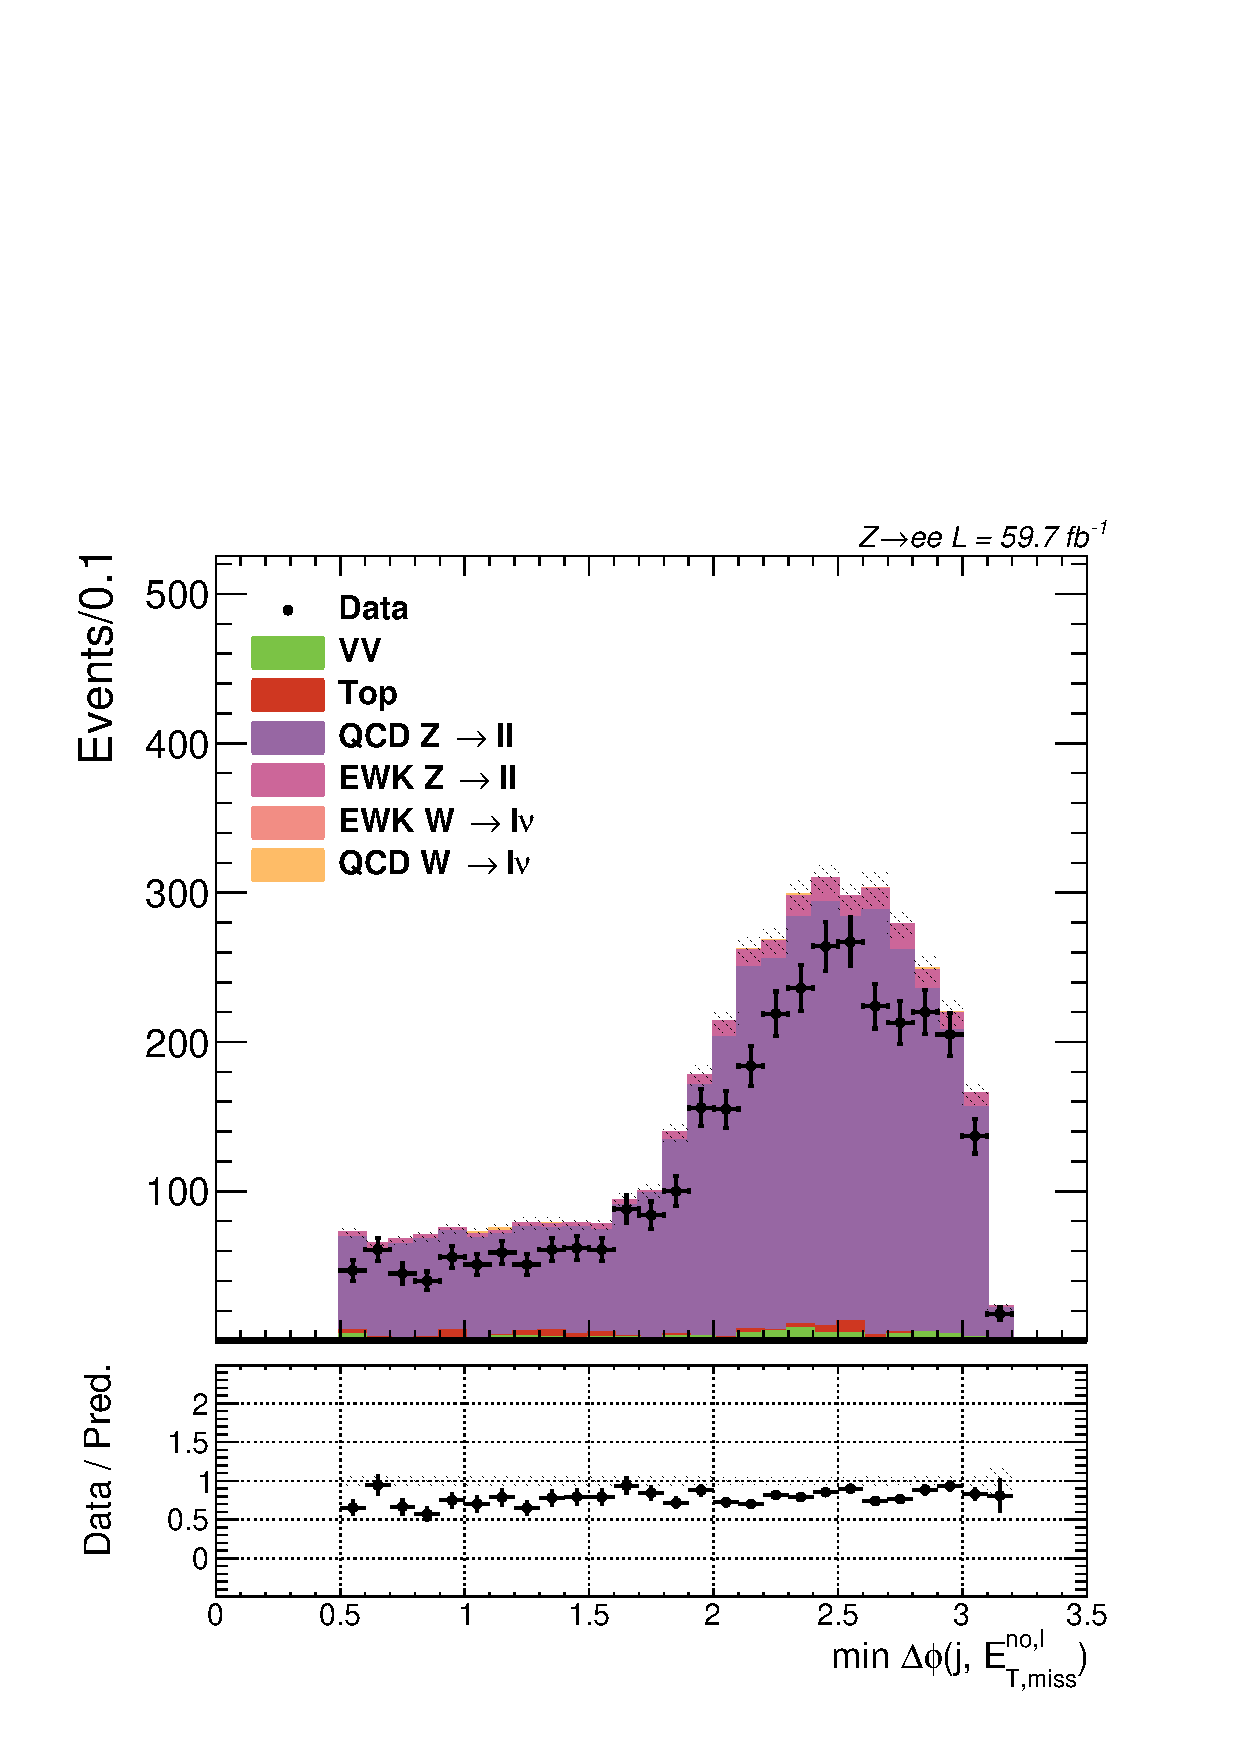
\includegraphics[width=0.49\textwidth]{Control_Regions/2018_MTR/Zee/MetNoLep_CleanJet_mindPhi.pdf}
    }\\
    \subfigure[$E_{T,miss}$ - VTR]{
    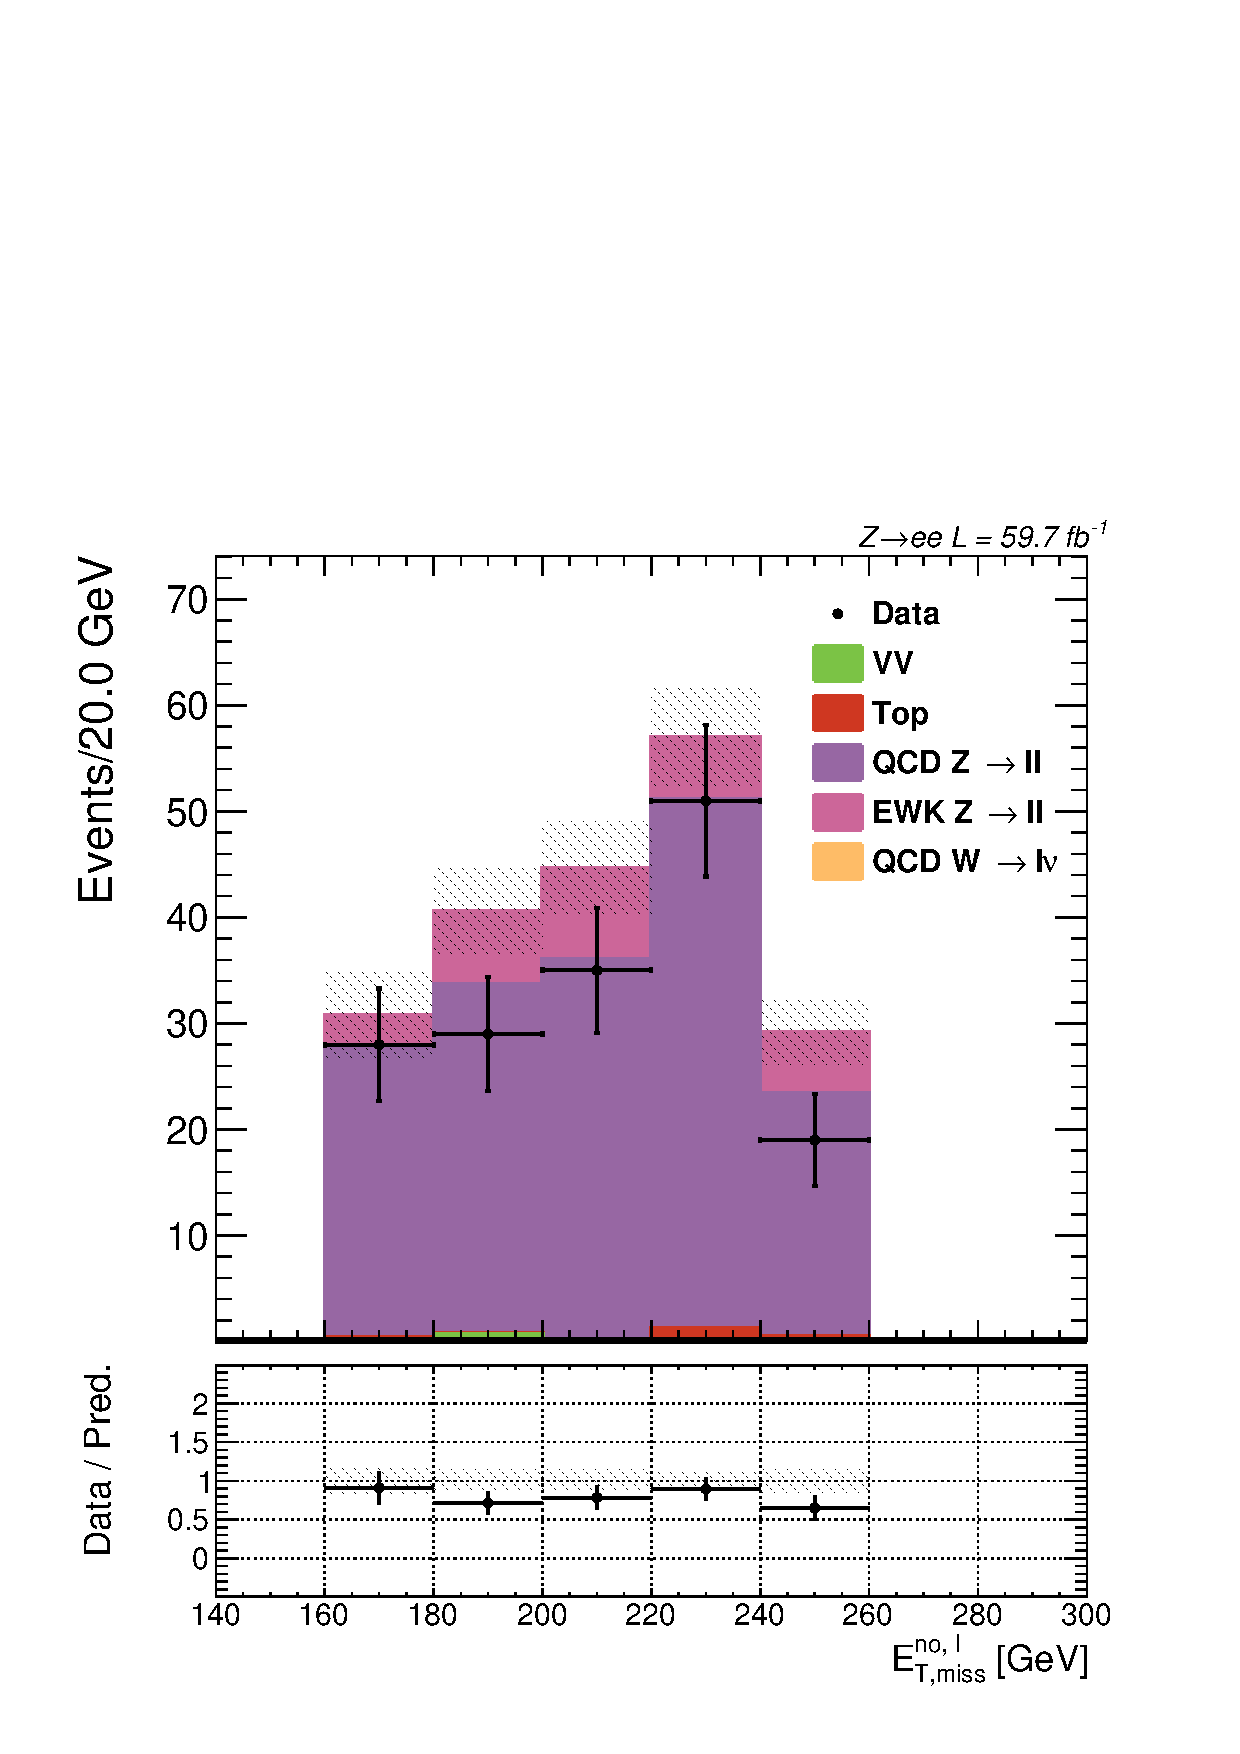
\includegraphics[width=0.49\textwidth]{Control_Regions/2018_VTR/Zee/MetNoMu.pdf}
    }
    \subfigure[$min\Delta\phi(j,E_{T,miss})$ - VTR]{
    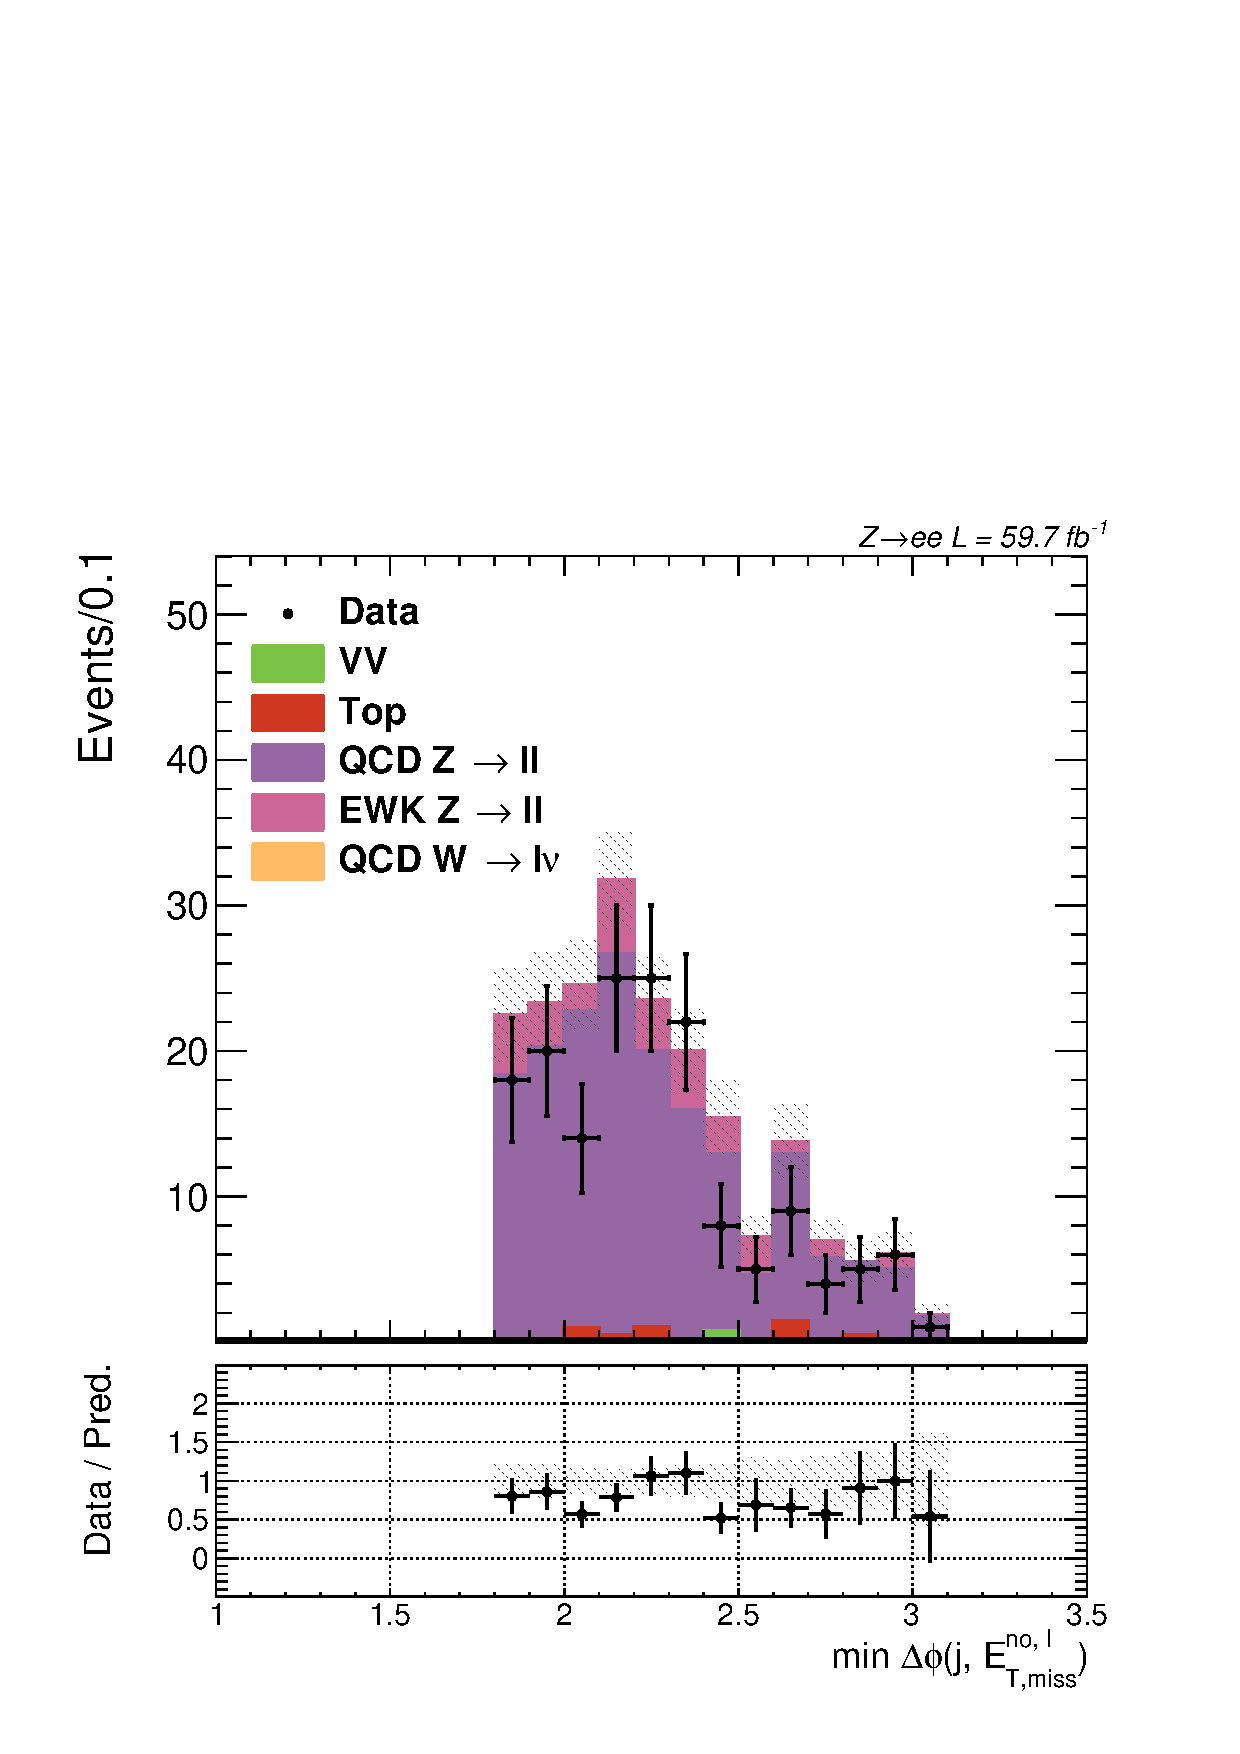
\includegraphics[width=0.49\textwidth]{Control_Regions/2018_VTR/Zee/MetNoLep_CleanJet_mindPhi.pdf}
    }
  \caption{Distributions of $E_{T,miss}$ and $min\Delta\phi(j,E_{T,miss})$ variables in the double muon region for MTR (top) and VTR (bottom) categories for the 2018 era of data taking.}
  \label{fig:2018_Zee_2}
\end{figure}


\subsection{Single Electron}
\label{sec:single_electron}
\hspace{10pt} There is one final lepton region left to define, the single electron region, which proves to be the most interesting one. It requires the modification of the electron veto, in order to select events with only one electron object that passes the tight requirements and passes the $p_T$ threshold of being larger than 40~GeV. In order to fight the contribution originating from QCD multijet processes a selection requirements of $E_{T,miss}>$~50~GeV was imposed.

\hspace{10pt} Looking at the 2018 era, the HEM problem started affecting this CR as well as the SR. With the lack of a tight $m_{ll}$ requirements, such as the Z mass window used for the dilepton regions, an effect was bound to show in the electron $\eta/\phi$ distributions. This is confirmed by Figure~\ref{fig:2018_Wenu_HEM}, which shows both of these variables. It can be seen that there is a large excess in data coming from the affected region which is not found in the simulation. This is a direct result of a lack of the HE information in the HEM region. Objects that would have been reconstructed as jets have the larger probability to fake an electron, creating large spikes seen in $\eta/\phi$ distributions.

\hspace{10pt} There are two approaches that can be taken at this stage. The first one, also the simpler one, is to effectively veto events that have an electron in the HEM region. This translated into a veto range of $\eta <$~-1.3 and -1.6~$\leq\phi\leq$~-0.9. Alternative approach would be to redefine the electron collection by removing the objects which are found in the affected region. This option provided no improvements over the first approach, leading to the simpler, veto approach being chosen. This was due to the fact that events gained were mostly originating from QCD multijet processes, hence being unable to successfully satisfy the tight requirements of MTR/VTR jet selection.

\hspace{10pt} Figures~\ref{fig:2017_Wenu_1} and~\ref{fig:2018_Wenu_1} show the $m_{jj}$ and $E_{T,miss}^{no,e}$ distributions for 2017 and 2018 era respectively, with the $m_{jj}$ having a good agreement between data and simulation for all eras. Additionally, the $M_{T,e}$ (computed from $\vec{p}_{T.miss}$ and the electron $p_T$) and \mindphinoe~data to simulation comparisons are shown in Figures~\ref{fig:2017_Wenu_2} and~\ref{fig:2018_Wenu_2} for both categories and eras. Additional distributions related to this region are given in Appendix~\ref{app:CRs}. 

\hspace{10pt} Story of the background extraction using these four lepton regions is going to be one of the main focuses of Chapter~\ref{ch:fit}, where they will be included in the final fit through the usage of transfer factors connecting CRs with the final SR estimation.


\begin{figure}[htbp]
  \centering
    \subfigure[$\eta_e$ - pre veto]{
    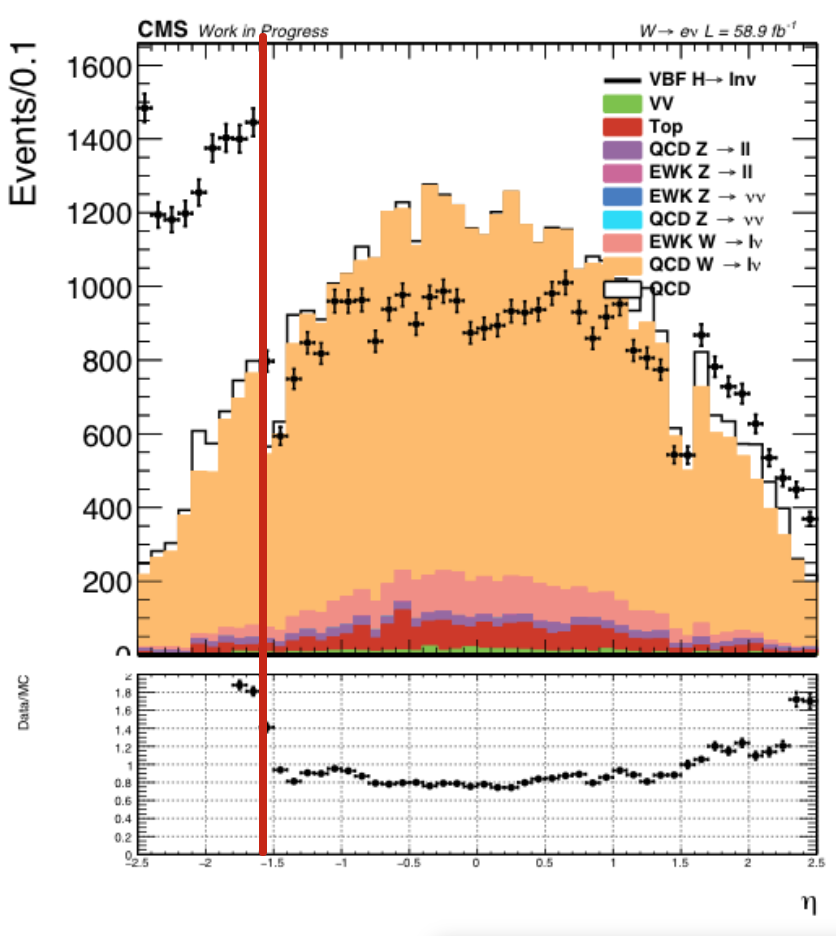
\includegraphics[width=0.49\textwidth]{Control_Regions/HEM_motivation/Ele_eta_preVeto2018.png}
    }
    \subfigure[$\phi_e$ - pre veto]{
    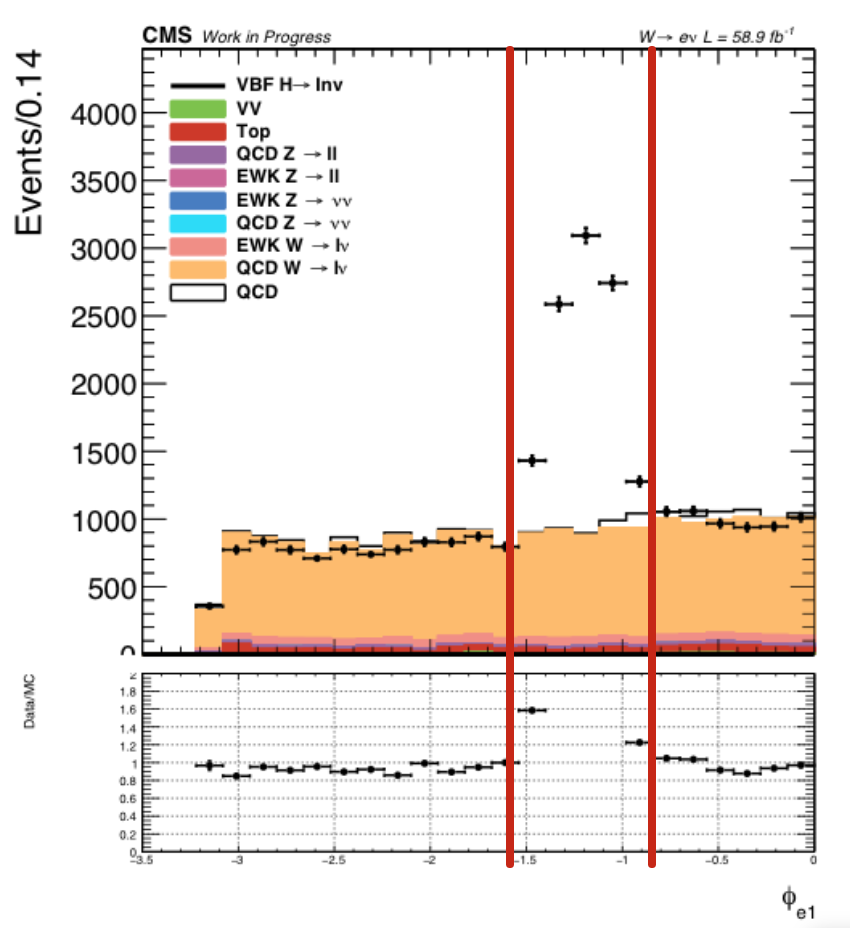
\includegraphics[width=0.49\textwidth]{Control_Regions/HEM_motivation/Ele_phi_preVeto2018.png}
    }\\
    \subfigure[$\eta_e$ - post veto]{
    \includegraphics[width=0.49\textwidth]{Control_Regions/HEM_motivation/Ele_eta_postVeto2018.png}
    }
    \subfigure[$\phi_e$ - post veto]{
    \includegraphics[width=0.49\textwidth]{Control_Regions/HEM_motivation/Ele_phi_postVeto2018.png}
    }
  \caption{Distribution of electron $\eta$ and $\phi$ variables showing the pre (top) and post (bottom) veto mitigation results (presented for the MTR category).}
  \label{fig:2018_Wenu_HEM}
\end{figure}





\begin{figure}[htbp]
  \centering
    \subfigure[$m_{jj}$ - MTR]{
    \includegraphics[width=0.49\textwidth]{Control_Regions/2017_MTR/Wenu/leadingJet_mjj.pdf}
    }
    \subfigure[$E_{T,miss}$ - MTR]{
    \includegraphics[width=0.49\textwidth]{Control_Regions/2017_MTR/Wenu/MetNoMu.pdf}
    }\\
    \subfigure[$m_{jj}$ - VTR]{
    \includegraphics[width=0.49\textwidth]{Control_Regions/2017_VTR/Wenu/lMjj.pdf}
    }
    \subfigure[$E_{T,miss}$ - VTR]{
    \includegraphics[width=0.49\textwidth]{Control_Regions/2017_VTR/Wenu/MetNoMu.pdf}
    }
  \caption{Distributions of $mjj$ and $E_{T,miss}$ variables in single electron region for MTR (top) and VTR (bottom) categories for the 2017 era of data taking.}
  \label{fig:2017_Wenu_1}
\end{figure}

\begin{figure}[htbp]
  \centering
    \subfigure[$m_{jj}$ - MTR]{
    \includegraphics[width=0.49\textwidth]{Control_Regions/2018_MTR/Wenu/leadingJet_mjj.pdf}
    }
    \subfigure[$E_{T,miss}$ - MTR]{
    \includegraphics[width=0.49\textwidth]{Control_Regions/2018_MTR/Wenu/MetNoMu.pdf}
    }\\
    \subfigure[$m_{jj}$ - VTR]{
    \includegraphics[width=0.49\textwidth]{Control_Regions/2018_VTR/Wenu/lMjj.pdf}
    }
    \subfigure[$E_{T,miss}$ - VTR]{
    \includegraphics[width=0.49\textwidth]{Control_Regions/2018_VTR/Wenu/MetNoMu.pdf}
    }
  \caption{Distributions of $mjj$ and $E_{T,miss}$ variables in single electron region for MTR (top) and VTR (bottom) categories for the 2018 era of data taking.}
  \label{fig:2018_Wenu_1}
\end{figure}


\begin{figure}[htbp]
  \centering
    \subfigure[$M_{T,e}$ - MTR]{
    \includegraphics[width=0.49\textwidth]{Control_Regions/2017_MTR/Wenu/MTe_FAST.pdf}
    }
    \subfigure[\mindphinoe - MTR]{
    \includegraphics[width=0.49\textwidth]{Control_Regions/2017_MTR/Wenu/MetNoLep_CleanJet_mindPhi.pdf}
    }\\
    \subfigure[$M_{T,e}$ - VTR]{
    \includegraphics[width=0.49\textwidth]{Control_Regions/2017_VTR/Wenu/MTe_FAST.pdf}
    }
    \subfigure[\mindphinoe - VTR]{
    \includegraphics[width=0.49\textwidth]{Control_Regions/2017_VTR/Wenu/MetNoLep_CleanJet_mindPhi.pdf}
    }
  \caption{Distributions of $M_{T,e}$ and \mindphinoe variables in single electron region for MTR (top) and VTR (bottom) categories for the 2017 era of data taking.}
  \label{fig:2017_Wenu_2}
\end{figure}

\begin{figure}[htbp]
  \centering
    \subfigure[$M_{T,e}$ - MTR]{
    \includegraphics[width=0.49\textwidth]{Control_Regions/2018_MTR/Wenu/MTe_FAST.pdf}
    }
    \subfigure[\mindphinoe - MTR]{
    \includegraphics[width=0.49\textwidth]{Control_Regions/2018_MTR/Wenu/MetNoLep_CleanJet_mindPhi.pdf}
    }\\
    \subfigure[$M_{T,e}$ - VTR]{
    \includegraphics[width=0.49\textwidth]{Control_Regions/2018_VTR/Wenu/MTe_FAST.pdf}
    }
    \subfigure[\mindphinoe - VTR]{
    \includegraphics[width=0.49\textwidth]{Control_Regions/2018_VTR/Wenu/MetNoLep_CleanJet_mindPhi.pdf}
    }
  \caption{Distributions of $M_{T,e}$ and \mindphinoe variables in single electron region for MTR (top) and VTR (bottom) categories for the 2018 era of data taking.}
  \label{fig:2018_Wenu_2}
\end{figure}





\section{Dedicated QCD multijet region}

\hspace{10pt} The main reason behind the problematic nature of QCD multijet processes is their high production rate at the LHC. They are not expected to contain a lot of events with the ability to pass the MTR/VTR selection requirements (especially due to the existence of the \mindphi~threshold), as they usually produce events which are well balanced in the transverse plane. Unfortunately, any mismeasurement of jet energy, poorly functioning detector regions or neutrinos from semileptonic decays of heavy-flavour mesons, coupled with large cross sections values, result in a non negligible amount of them containing VBF-like signature (energetic leading/subleading jets accompanied with a large $E_{T,miss}$ originating from these edge cases). 

\hspace{10pt} Their contribution is significantly reduced in the lepton CRs through the usage of the \mindphi~variable. In order to properly estimate this contribution in the SR (also bypassing the low statistics of simulation samples, by not relying simply on them), an extrapolation approach was deployed through the usage of a region which is considered "enriched" by these processes. The following pages are going to define this region and to present two approaches, one of which will be used as the final estimation, while the other being used as a cross check.

\subsection{Definition}

\hspace{10pt} The importance of the \mindphi~variable can be seen in its connection to QCD multijet processes. If there is a jet energy mismeasurement for a process which is expected to be a well balanced one, the $\vec{p}_{T,miss}$ is going to be influenced by the direction of those missmeasured jets. The low \mindphi~range provides a good handle when creating a region largely populated by multijet processes, which can, in return, be used to estimate their contribution in the SR. This difference between two sections (low and high \mindphi) can be expressed as:

\begin{equation}
    r = \frac{min\Delta\phi(j, E_{T,miss})>X}{min\Delta\phi(j, E_{T,miss})<X},
\end{equation}
where X denotes the threshold corresponding to each category, taking the value of 0.5 (1.8) for MTR (VTR) category respectively.

\hspace{10pt} In order to obtain the estimation of the SR-related contribution, as well as to perform a set of closure tests, four orthogonal regions are introduced. They are defined with slight modifications of the MTR (VTR) selection by inverting the $min\Delta\phi(j, E_{T,miss})$ and $E_{T,miss}$ requirements, as shown in Table~\ref{tab:QCD_regions}.

\begin{table}[htbp]
\centering
\small
\begin{tabular}{lc}
\hline\hline
Name & Definition\\\hline
Region A &  $min\Delta\phi(j, E_{T,miss})<$0.5 (1.8) and 100$<E_{T,miss}<$160~GeV \\
Region B & $min\Delta\phi(j, E_{T,miss})>$0.5 (1.8) and 100$<E_{T,miss}<$160~GeV   \\
QCD CR   & $min\Delta\phi(j, E_{T,miss})<$0.5 (1.8) and $E_{T,miss}>$250~GeV ($\in$[160, 250)~GeV)   \\
Signal Region &  $min\Delta\phi(j, E_{T,miss})>$0.5 (1.8) and $E_{T,miss}>$250~GeV ($\in$[160, 250)~GeV)   \\

\hline\hline
\end{tabular}
\caption{Definition of four regions used for the estimation of the total contribution of QCD multijet processes in the SR. Thresholds are presented for MTR (VTR) category respectively.\label{tab:QCD_regions} }
\end{table}

\hspace{10pt} For the purposes of this analysis two methods are going to be tested. Both of them are going to be summarised in the following pages. First of them depends both on the simulation samples and data, while the second one lacks the dependence on the simulated QCD multijet processes (making it the preferred option, due to the lack of statistics in the simulation samples).

\subsection{Method A}
\hspace{10pt} The basis for this method is built around the, previously defined, factor $r$. Due to the analysis relying on the $m_{jj}$ variable for the final fit, its definition will be expanded to appropriately reflect dependence on the dijet mass. It can be expressed in terms of $m_{jj}$ bins as: 
\begin{equation}
    r(m_{jj}) = \frac{F_{SR}^{MC}(m_{jj})}{F_{QCD~CR}^{MC}(m_{jj})},
\end{equation}
where the $F^{MC}_i$ denotes the $m_{jj}$ distributions of QCD multijet simulation samples in the QCD CR and SR.

\hspace{10pt} Due to the lack of statistics in respective simulation samples, some thresholds in the VBF selection had to be loosened in order for this method to produce sensible output. This resulted in a relaxed, $\Delta\phi_{jj}<$~2.5, requirement being introduced when computing $r(m_{jj})$. The final multijet contribution in the SR is obtained, by translating the data driven estimation in the CR using the $r(m_{jj})$, through the usage of the following formula:

\begin{equation}
    N_{SR}^{QCD}(m_{jj}) = \left( N_{CR}^{Data}(m_{jj}) - \sum_i N^i_{CR}(m_{jj})\right)\cdot r(m_{jj}),
\end{equation}

where the sum goes over other backgrounds (V+jets, now a minor background in this region, $t\bar{t}$ and diboson processes). Following the heavy dependence on the simulation sample (and due to its the lack of statistics), a more favourable method was searched for that would be only data driven. The following paragraphs define this method and its usage in further analysis steps.

\subsection{Method B}
\hspace{10pt} Alternative approach to method A is to remove the dependence on the QCD multijet simulation and instead rely only on a purely data driven estimation. For the purposes of this method, a fit procedure is deployed on the $min\Delta\phi(j, E_{T, miss})$ in its low region. The resulting fit function enables the extrapolation into the SR.

\hspace{10pt} Firstly, in order to have a good handle on the contribution of other backgrounds in the, QCD enriched, low $min\Delta\phi(j, E_{T, miss})$ region, a fit is performed on the combined contribution of V+jets, diboson and $t\bar{t}$ simulation samples. This action is performed using a fit function defined as:
\begin{equation}
    F_B(x)  = Q_0e^{-Q_1x}(1+Q_2x+Q_3x^2),
\end{equation}
where $Q_i$ denotes fit parameters, while $x$ represents the fit variable (in this situation $min\Delta\phi(j, E_{T, miss})$). Following these studies, the next step is to fit the data using a fit function defined as:
\begin{equation}
    F(x) = F_B(x)+F_{QCD}(x) = Q_0e^{-Q_1x}(1+Q_2x+Q_3x^2)+P_0e^{-P_1x}+P_2,
\end{equation}
where the $P_i$ represent the new fit parameters. Through the usage of the information gained by fitting the smaller backgrounds, parameters $Q_i$ are fixed when performing the fit in data, thus allowing for the definition of the $F_{QCD}(x)$ through the remaining $P_i$ parameters. In order to estimate the total contribution coming from QCD multijet processes in the SR, this newly obtained function $F_{QCD}(x)$ can be integrated over the SR, or in other words:
\begin{equation}
    N_{QCD}^{SR} = \int_X^{\pi}F_{QCD}(x)dx,
\end{equation}
where the lower bound X takes the value of 0.5 (1.8) for MTR (VTR) category respectively. The actual implementation requires a separate fir procedure per category for each era. For the MTR category, a fit range of 0~$\leq min\Delta\Phi(j,E_{T,miss})\leq$~1.0 is chosen, while the 0.5~$\leq min\Delta\Phi(j,E_{T,miss})\leq$~1.0 range covers the VTR category fit strategy. The extended fit range used for the MTR category is enabled through the partial unblinding strategy defined in Section~\ref{sec:data_quality} and supported by the fact that this range is not expected to have any significant signal contribution.

\hspace{10pt} One important remark regarding this option is the statement that it builds itself from the fact that the dijet mass isn't strongly correlated with with $min\Delta\Phi(j,E_{T,miss})$. This is going to be supported by the distribution $r(m_{jj})$ from the implementation process of method A, but more details about these results are going to be given in Chapter~\ref{ch:fit}, where the background estimation is explained in more detail.

\hspace{10pt} The final step is to translate this information into the final SR contribution from the point of view of the $m_{jj}$ variable. The overall normalisation of the QCD multijet SR contribution is there, the only thing which remains is to determine the shape of the distribution. Due to the aforementioned small correlation between the two variables, this can be achieved by looking into the QCD CR and subtracting the contribution of other background from data. Upon obtaining the resulting $m_{jj}$ distribution, the only thing left to do is to scale it to the proper normalisation, which in this case is represented by the value of $N_{QCD}^{SR}$.

\hspace{10pt} As previously mentioned, the following chapter is going to focus on the practical implementation of these CRs into the analysis flow and their associated uncertainties, serving as a companion piece concluding the story of background processes from the point of view of this study.

